% Sample Dissertation, Thesis, or Document %
%            for use with the              %
%  University of Arizona Thesis Class,     %
%               uathesis.cls               %
%------------------------------------------%

% We'll use the uathesis document class (duh).  The uncommented line
% below will produce a Dissertation, the others would produce a Thesis
% or a Document.  There are other options available to you like turning
% on the copyright statement and replacing the year on the title page
% with a "generated on" stamp (handy for early drafts).  To find out
% what the available options are, take a look into the uathesis.cls
% file and look for the \DeclareOption commands near the top of that
% file.
% There are five copyright options.  Copyright, no copyright, and three
% different Creative Commons licences.  Use the one you want (If you go
% Creative Commons, I (DM) think the CC-BY-ND makes the most sense)  See
% uathesis.cls for the reason why the non-commercial licenses are not
% included.
%\documentclass[dissertation]{uathesis}
\documentclass[dissertation,copyright]{uathesis}\usepackage[]{graphicx}\usepackage[]{color}
%% maxwidth is the original width if it is less than linewidth
%% otherwise use linewidth (to make sure the graphics do not exceed the margin)
\makeatletter
\def\maxwidth{ %
  \ifdim\Gin@nat@width>\linewidth
    \linewidth
  \else
    \Gin@nat@width
  \fi
}
\makeatother

\definecolor{fgcolor}{rgb}{0.345, 0.345, 0.345}
\newcommand{\hlnum}[1]{\textcolor[rgb]{0.686,0.059,0.569}{#1}}%
\newcommand{\hlstr}[1]{\textcolor[rgb]{0.192,0.494,0.8}{#1}}%
\newcommand{\hlcom}[1]{\textcolor[rgb]{0.678,0.584,0.686}{\textit{#1}}}%
\newcommand{\hlopt}[1]{\textcolor[rgb]{0,0,0}{#1}}%
\newcommand{\hlstd}[1]{\textcolor[rgb]{0.345,0.345,0.345}{#1}}%
\newcommand{\hlkwa}[1]{\textcolor[rgb]{0.161,0.373,0.58}{\textbf{#1}}}%
\newcommand{\hlkwb}[1]{\textcolor[rgb]{0.69,0.353,0.396}{#1}}%
\newcommand{\hlkwc}[1]{\textcolor[rgb]{0.333,0.667,0.333}{#1}}%
\newcommand{\hlkwd}[1]{\textcolor[rgb]{0.737,0.353,0.396}{\textbf{#1}}}%
\let\hlipl\hlkwb

\usepackage{framed}
\makeatletter
\newenvironment{kframe}{%
 \def\at@end@of@kframe{}%
 \ifinner\ifhmode%
  \def\at@end@of@kframe{\end{minipage}}%
  \begin{minipage}{\columnwidth}%
 \fi\fi%
 \def\FrameCommand##1{\hskip\@totalleftmargin \hskip-\fboxsep
 \colorbox{shadecolor}{##1}\hskip-\fboxsep
     % There is no \\@totalrightmargin, so:
     \hskip-\linewidth \hskip-\@totalleftmargin \hskip\columnwidth}%
 \MakeFramed {\advance\hsize-\width
   \@totalleftmargin\z@ \linewidth\hsize
   \@setminipage}}%
 {\par\unskip\endMakeFramed%
 \at@end@of@kframe}
\makeatother

\definecolor{shadecolor}{rgb}{.97, .97, .97}
\definecolor{messagecolor}{rgb}{0, 0, 0}
\definecolor{warningcolor}{rgb}{1, 0, 1}
\definecolor{errorcolor}{rgb}{1, 0, 0}
\newenvironment{knitrout}{}{} % an empty environment to be redefined in TeX

\usepackage{alltt}
%\documentclass[dissertation,CC-BY]{uathesis}
%\documentclass[dissertation,CC-BY-SA]{uathesis}
%documentclass[dissertation,CC-BY-ND]{uathesis}
%\documentclass[thesis]{uathesis}
%\documentclass[document]{uathesis}

% Package Usage
% These are the packages that we need
\usepackage{booktabs}
\usepackage{graphicx}
\usepackage{natbib}			% natbib is available on most systems, and is
					% terribly handy.
					
%May need to remove! Trying to fix nocite{*} biblography problem:
					% If you want to use a different Bibliography package, 
					% you should be able to, just change this
					% and the \bibliographystyle command below.  Be warned
					% that you may need to do a little hacking to get
					% the REFERENCES item to show up in your TOC.

% Compatibility with the AASTEX package 
% of the American Astronomical Society.
%\usepackage{deluxetable}		% Allows use of AASTEX deluxe tables
%\usepackage{aastex_hack}		% Allows other AASTEX functionality.

% These are other packages that you might find useful.
% For controlling the fonts, see
% http://www.math.uiuc.edu/~hartke/computer/latex/survey/survey.html
% The following is a nice font set:
%\usepackage{mathtime}			% Times for letters; Belleek math.
%
\usepackage{wrapfig}

\newenvironment{lydiawrapfigure}
 {%
%  \setlength{\intextsep}{0pt}% <--- Wrong!
  \setlength{\columnsep}{15pt}%
  \wrapfloat{figure}%
 }
 {\endwrapfloat}
 
\usepackage{caption}
\usepackage{subcaption}
\usepackage{tipa}
\usepackage{color,soul}
\usepackage{url}
\usepackage{blindtext}
\usepackage[inline]{enumitem}
\usepackage{breakurl}
\usepackage{mathtools}
\usepackage{amsmath}
% \usepackage[normalem]{ulem}
% \usepackage{xyling,comment}			% AMS Math (advanced math typesetting)
% includecomment{delall}
% %\excludecomment{delall}
% 
% %default: don't show edits
% 
% \newcommand{\add}[1]{#1}
% \newcommand{\del}[1]{}
% \newcommand{\delni}[1]{}
% \newcommand{\addtab}{}
% 
% %block to show edits controlled by include/exclude-comment above
% \begin{delall}
% %added stuff
% \renewcommand{\add}[1]{\textcolor{blue}{#1}}
% %added table
% \renewcommand{\addtab}{\color{blue}}
% %deleted stuff
% \renewcommand{\del}[1]{\textcolor{red}{\sout{#1}}}
% \renewcommand{\delni}[1]{\noindent\textcolor{red}{\sout{#1}}}
% \end{delall}

%\usepackage{lscape}			% Used for making fitting large tables in by putting them landscape
%\usepackage{refs}			
%
% If you are using hyper-ref (recommended), this command must go after all 
% other package inclusions (from the hyperref package documentation).
% The purpose of hyperref is to make the PDF created extensively
% cross-referenced.

%Also works! Change dvips to driverfallback=dvips.
\usepackage[driverfallback=dvips,bookmarks,colorlinks=true,urlcolor=black,linkcolor=black,citecolor=black]{hyperref}


%Works!
%\usepackage[pdftex,bookmarks,colorlinks=true,urlcolor=black,linkcolor=black,citecolor=black]{hyperref}
%HERE IS THE THING THAT NEEDS TO CHANGE TO GET LATEX TO WORK WITH RSTUDIO. USE pdftex instead of dvips.

% Set up some values.
\completetitle{Working Title: An approach to automatic and human speech recognition using ear-recorded speech.}
\fullname{Samuel John Charles Johnston}			% Grad college wants your full name here.
\degreename{Doctor of Philosophy}	% Title of your degree.
\IfFileExists{upquote.sty}{\usepackage{upquote}}{}
\begin{document}


% Set up the title page
\maketitlepage
{DEPARTMENT OF LINGUISTICS}	% Title of your department.
{2017}							

% Insert the approval form.  Note that for electronic submission
% of your Ph. D. dissertation, you must bring *two* copies of the
% approval page to your final defense.  These must be signed by
% the committee.  Make two photocopies: one for Pam and the other
% for your records.  Then, bring the two signed originals to the
% graduate college when you submit the final version of the
% dissertation to the University of Arizona.
\approval
{7 August 2017}		% Defense Date	
{Mike Hammond}	% Dissertation Director
{Mike Hammond}	% 1st committee member
{Brad Story}		% 2nd committee member
{Natasha Warner}		% 3rd committee member
{David Velenovsky}		% 4th committee member
{}		% 5th committee member

% Include the ``Statement by Author'' for Dissertations
\statementbyauthor
% If this is a Thesis, use the following form, with your thesis director's
% name and title in the square brackets like so (you should also omit the 
% approval form insertion above):
%\statementbyauthor[Jane M. Doe\\Professor of Chemistry]

% Include the ``Acknowledgements''
\incacknowledgements{acknowledgements}

% Include the ``Dedication''
\incdedication{dedication}

% Create a ``Table of Contents''
\tableofcontents

% Create a ``List of Figures''
\listoffigures

% Create a ``List of Tables''
\listoftables

% Include the ``Abstract''
\incabstract{abstract}






% Include the various chapters:


%ADD: Copy/Paste Content from all 5 chapters:

% %set_parent(‘/Users/mwilli/Documents/Spring_2017/Dissertation_Document/Dissertation_Working_Directory_Draft/Dissertation_Main.Rnw')
% 
% <<chunk_options, echo=FALSE>>=
% # This is where we set basic knitr options.
% opts_chunk$set(echo=TRUE, message=FALSE, warning = FALSE, cache = FALSE, comment="")
% options(width=75) # This sets how wide the R printout can be.
% @
% 
%  <<setup-child, include=FALSE>>=
%  set_parent('/home/sam/Dissertation/Dissertation_Template/Dissertation_Main_Template/Dissertation_Main.Rnw')
% @
% 
% <<load_libraries, echo=FALSE>>=
% library(tidyr)
% library(dplyr)
% library(ggplot2)
% library(lme4)
% library(lsmeans)
% library(car)
% library(pbkrtest)
% library(xtable)
% library(cowplot)
% library(plyr)
% @

\chapter{Introduction\label{chapter1}}

Speech in a noisy background presents a challenge to the recognition of that speech both by human listeners and by computers tasked with recognizing human speech (termed automatic speech recognition).  Years of research have resulted in many solutions, though none so far have completely solved the problem.  Most approaches have taken the route of trying to remove noise from a signal that is already corrupted with noise.

This project presents a new approach to the problem.  It proposes that human speech can be recorded in a manner that largely eliminates the noise before it reaches the microphone recording the signal.  The microphone would be placed inside the ear canal of the speaker and would record speech as it is passed through the bone and tissue of the speaker's head.  The signal is expected to be distorted by passage through the head, but this distortion is hypothesized to be at least partially reversible.

Section \ref{ch1:background} below describes the basic acoustics of sound, leading up to a brief overview of sound in noise.  Chapter \ref{chapter2} discusses the collection of ear-recorded speech, Chapter \ref{chapter3} describes a human speech perception experiment using ear-recorded speech, and Chapter \ref{chapter4} outlines an experiment testing the ability of an automatic speech recognition system to accurately recognize ear-recorded speech.  At the end of this chapter, Section \ref{ch1:diss-overview} will give a more detailed overview of the rest of the dissertation.

\section{Background}\label{ch1:background}

Sound itself, along with the ability to perceive it, is a remarkable phenomenon.  Put simply, `sound' is the fluctuation of pressure in neighboring groups of particles over time. Most frequently sound is discussed in terms of the fluctuation of air pressure, because, as humans, we primarily receive sound into our ear canals through the medium of air, but sound can also travel through media of liquids and solids, or pass through any combination of the three.

There are primarily three components to sound: amplitude, frequency, and phase, which can be seen in Figure \ref{fig:basic-sound-wave}.  In a simple sound wave, the amplitude of sound corresponds to the peak intensity of the high pressure (and the lowest pressure) portions of a sound wave (cf. Fig. \ref{fig:basic-sound-amplitude}).  The frequency corresponds to the rate at which the high and low pressure portions of the signal fluctuate between one another (cf. Fig. \ref{fig:basic-sound-frequency}).  The phase of a wave is the location of the pressure level (relative to atmospheric pressure) in time (cf. Fig. \ref{fig:basic-sound-phase}).   

\begin{figure}[h!]
\begin{subfigure}{0.5\textwidth}
  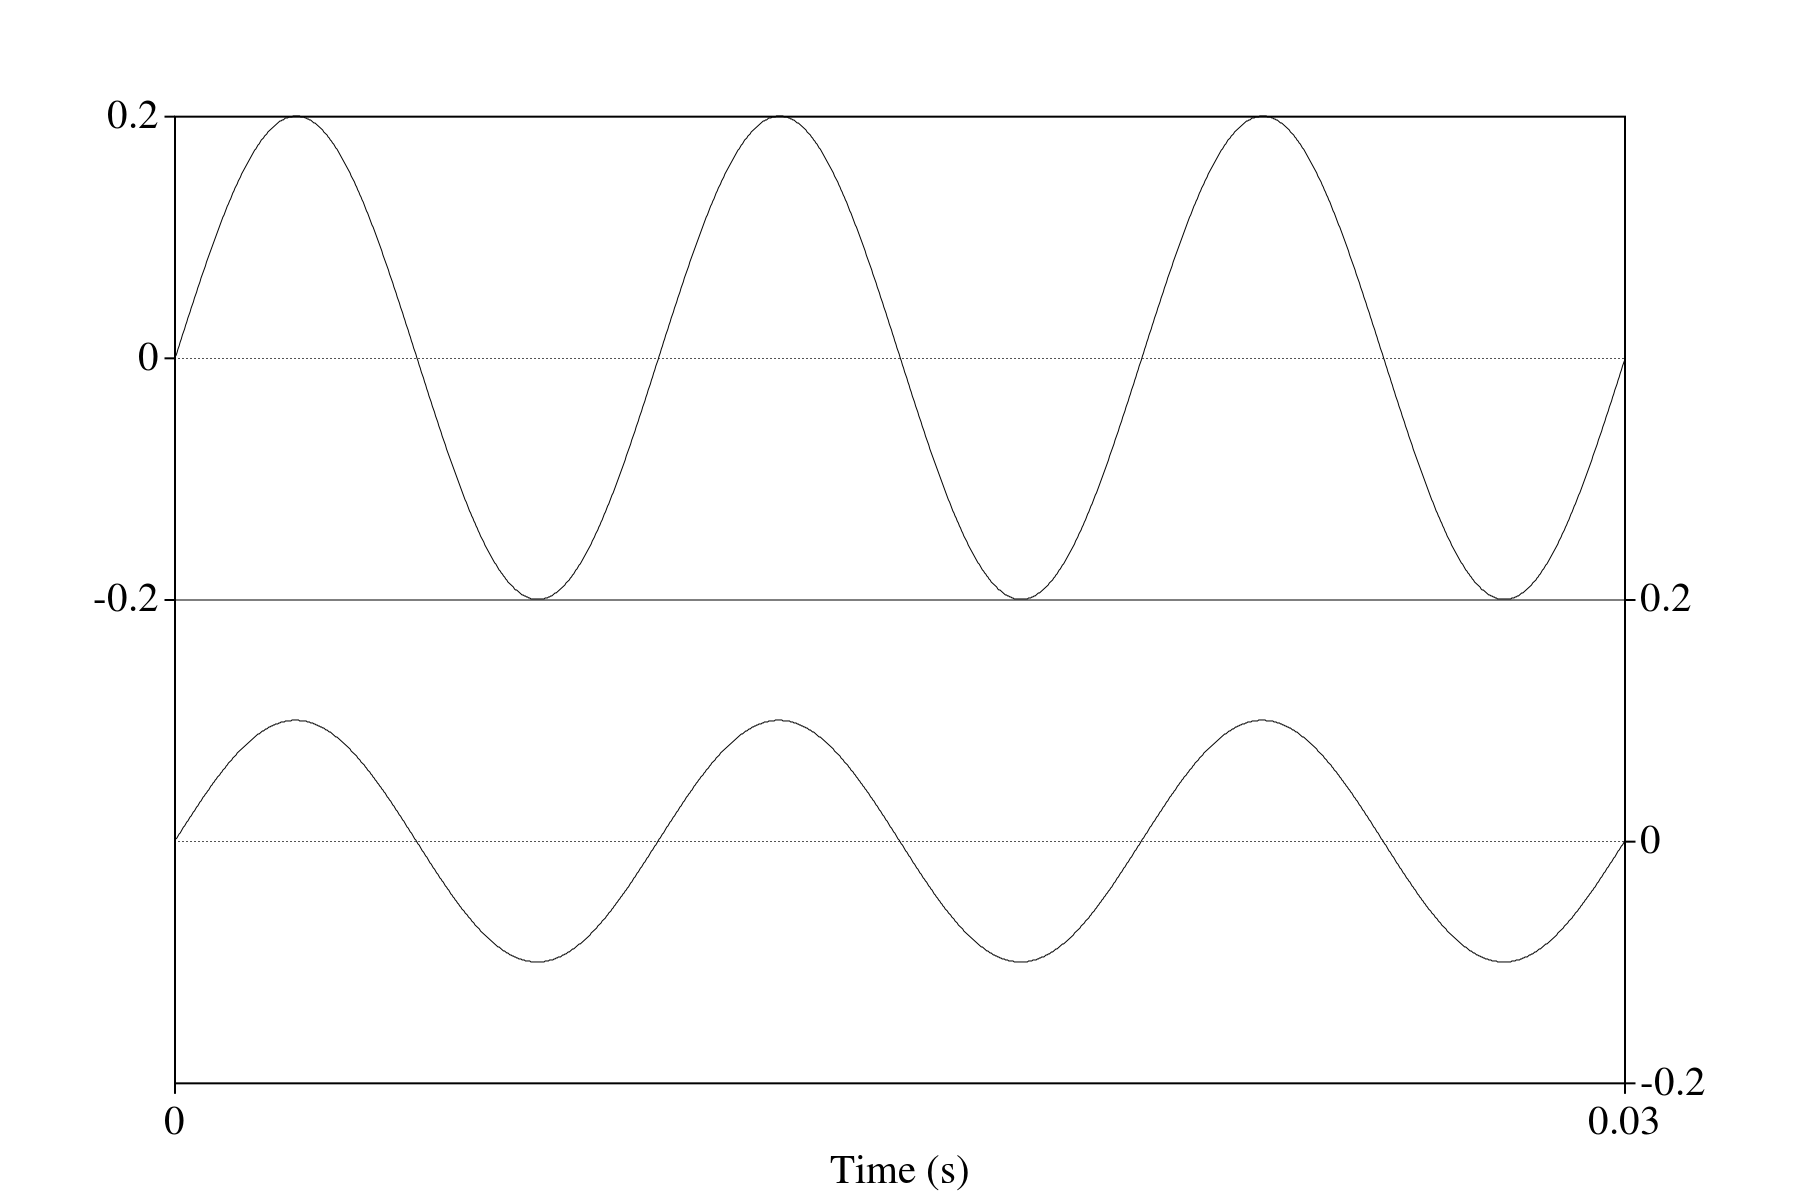
\includegraphics[width=\textwidth]{figure/basic-sound-amplitude.png}
  \caption{Two waveforms showing a difference in amplitude between the two signals.}
  \label{fig:basic-sound-amplitude}
\end{subfigure}
\qquad
\begin{subfigure}{0.5\textwidth}
  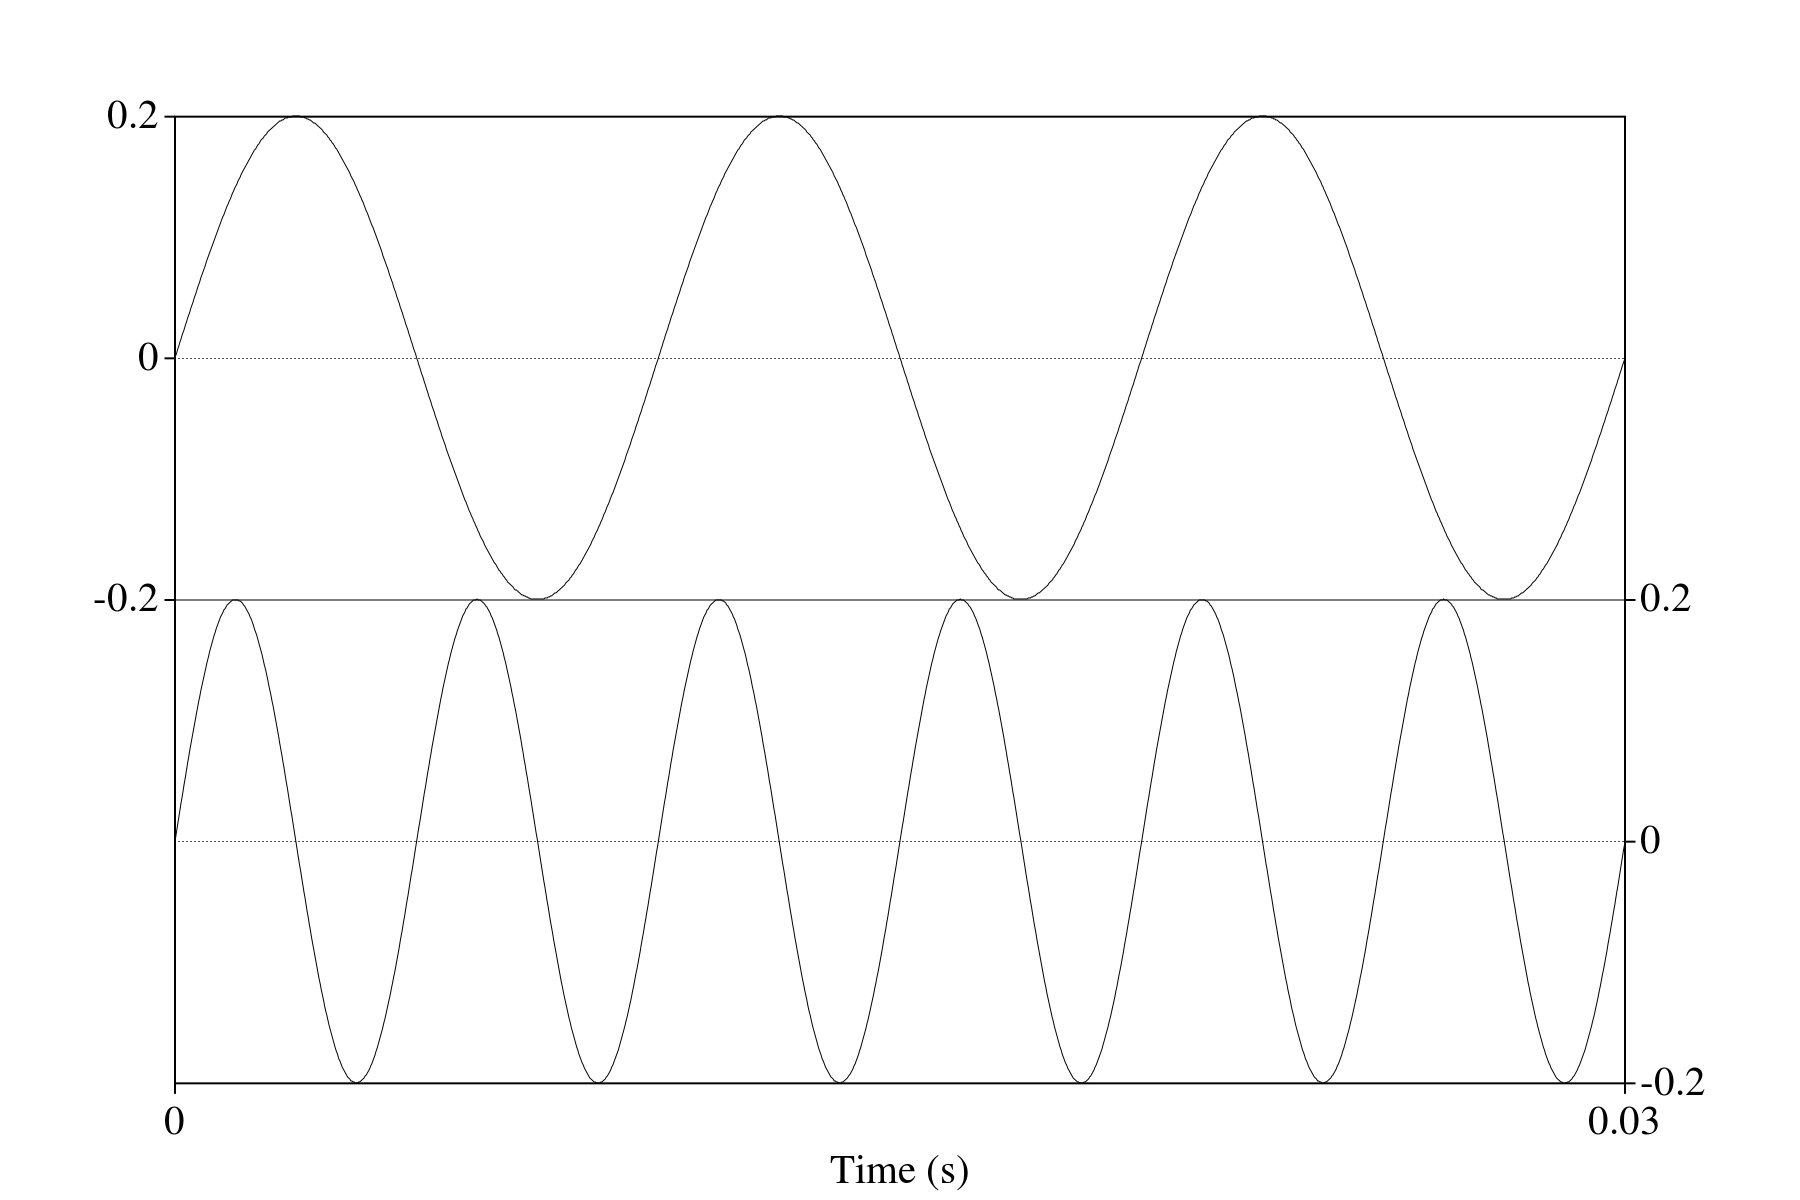
\includegraphics[width=\textwidth]{figure/basic-sound-frequency.png}
  \caption{Two waveforms showing a difference in frequency between the two signals.}
  \label{fig:basic-sound-frequency}
\end{subfigure}
%
\\[2ex]
\begin{center}
\begin{subfigure}{0.5\textwidth}
  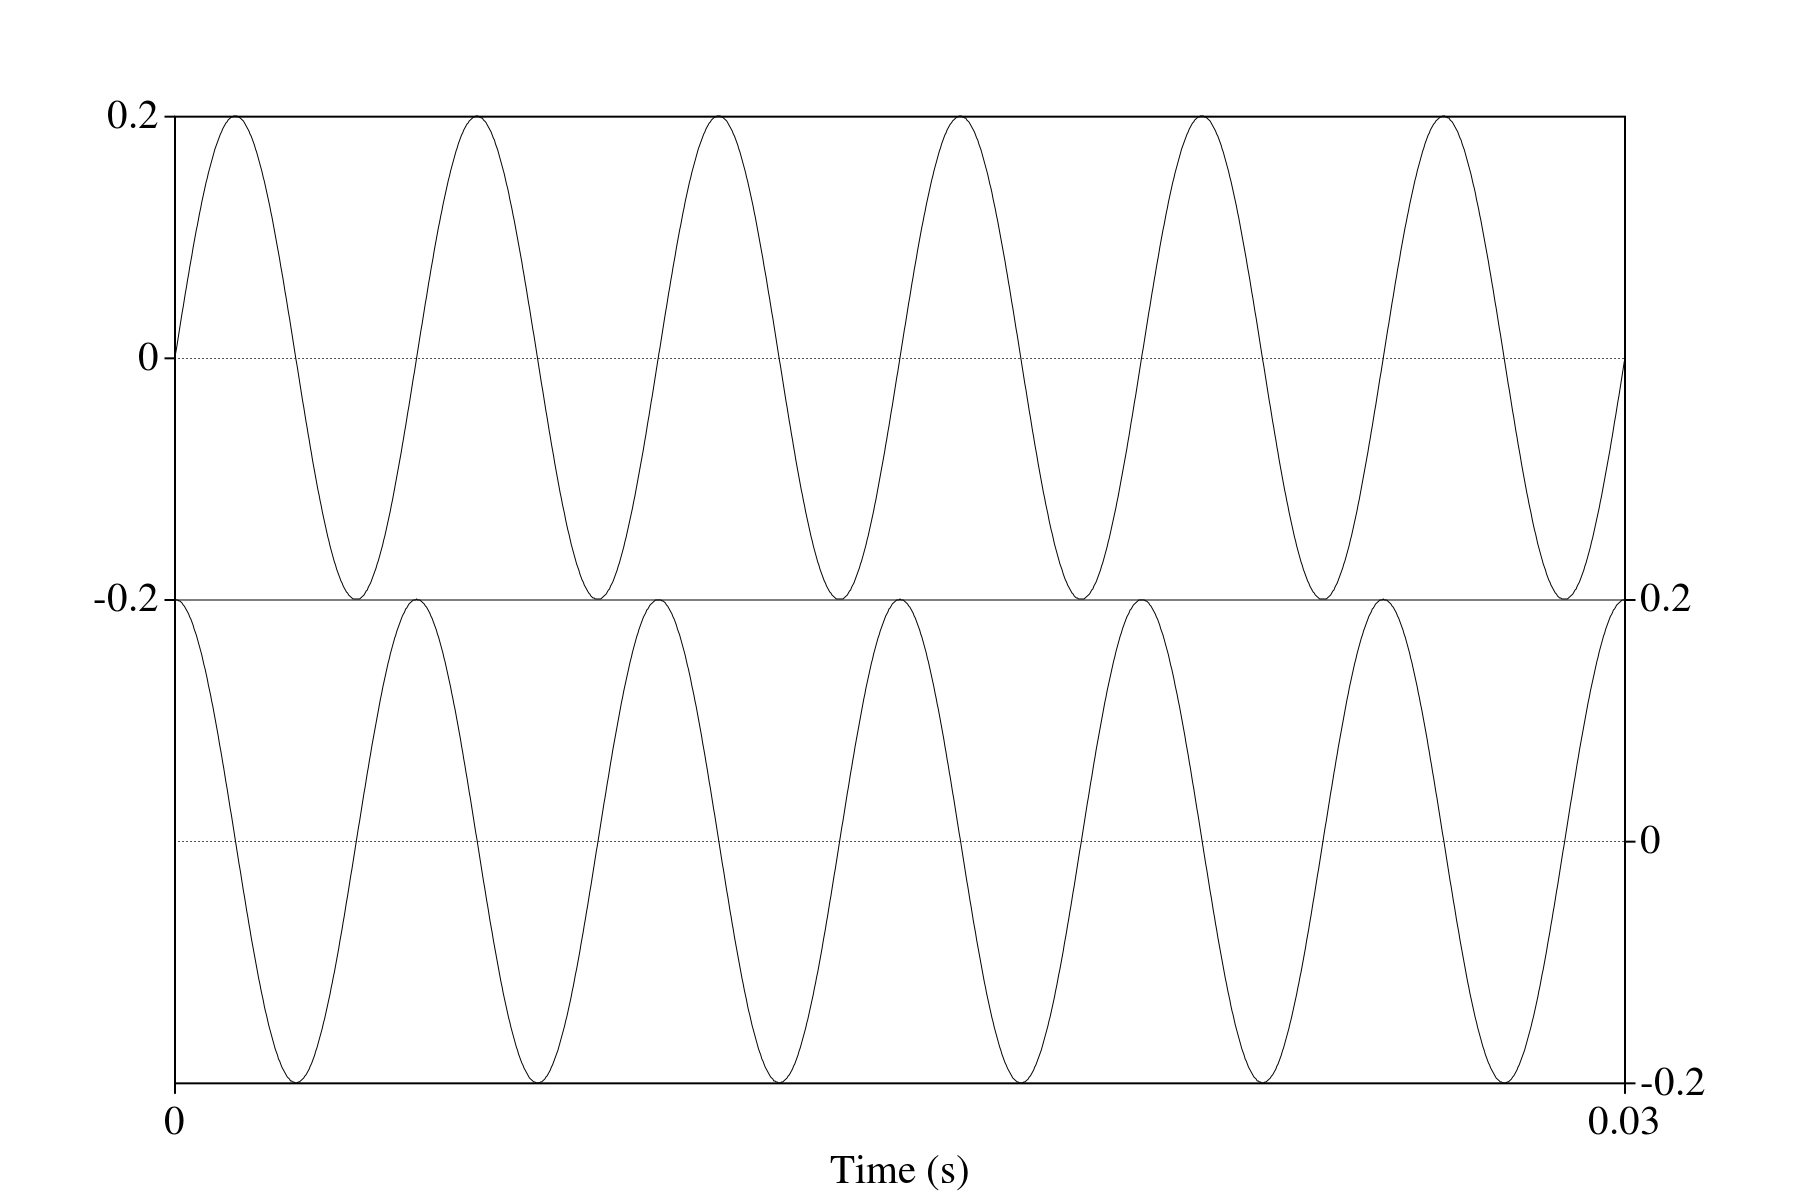
\includegraphics[width=\textwidth]{figure/basic-sound-phase.png}
  \caption{Two waveforms showing a difference in phase between the two signals.}
  \label{fig:basic-sound-phase}
\end{subfigure}
\end{center}
\caption{Waveforms demonstrating difference in amplitude, frequency, and phase.}
\label{fig:basic-sound-wave}
\end{figure}

This latter characteristic - phase, while important when dealing with interacting waves from multiple sources, is often not taken into in speech science due to both its complexity and the fact that phase does not encode any speech information.  The human auditory system primarily makes use of the other two characteristics of sound - amplitude and frequency.

\subsection{Overview of Anatomy and Physiology of the Peripheral Auditory System}

Prior to discussing the acoustic structure of speech, it is important to become familiar with the basic peripheral auditory system.  The peripheral auditory system is generally grouped into three primary categories, the outer ear, the middle ear, and the inner ear (cf. Figure \ref{fig:ear-anatomy}).  The outer ear includes the pinna, the ear canal tube, and the tympanic membrane (ie. the eardrum).  Air-transmitted sound vibrations, ie. pressure fluctuations, enter the ear canal through the opening at the pinna.  These then travel along the canal to vibrate the tympanic membrane, which passes the energy to the middle ear.  The middle ear includes the ossicles within the middle ear cavity.  The ossicles are a chain of three very small bones leading from the tympanic membrane to the cochlea. The external sound vibrations hit the tympanic membrane, are passed along the ossicle chain, which then sends these vibrations to the inner ear.

\begin{figure}[h]
\centering
  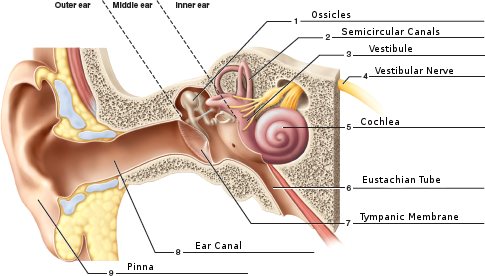
\includegraphics{figure/ear_anatomy.png}
  \caption{A diagram of the peripheral auditory system, including the outer ear, middle ear, and inner ear, up to the auditory nerve. (Image from \cite{martin:12})}
  \label{fig:ear-anatomy}
\end{figure}

The inner ear is composed of the cochlea, the semicircular canals (and vestibule), and the auditory and vestibular nerves.  The semicircular canals, vestibule, and vestibular nerve don't play a part in audition (their primary function regards balance sensitivity).  The cochlea, a hard `shell' filled with fluid receives the vibrations passed along through the middle ear ossicles.\footnote{The peripheral auditory system uses gas, solid, and liquid media to transmit acoustic vibrations.}  The vibrations are passed into the fluid cochlea and travel along the length of the cochlea, transmitting acoustic energy to cells that are able to detect the amplitude of the vibrations.  Depending on the location of a cell along the length of the cochlea, it will pick up a different frequency of sound.  The auditory nerve carries electrical impulses from these cells into the auditory cortex of the brain. 

Of interest to this present study is the relatively simple outer ear.  Typically, as described above, vibrations from the air will enter the ear canal through the opening at the pinna. Frequently, these vibrations take the form of human speech.

%However, vibrations from one's own speech are also transmitted via the bone, cartilage, and tissue of the head.  Regardless of source, sound vibrations entering into the ear canal will be altered by the shape of the ear canal, described more below.


\subsection{Acoustic Structure of Human Speech}

The structure of human speech draws from a collection of individual sounds (phonemes) that are strung together, encoding words, sentences, and more abstractly, meaning.  Each human language uses a subset of all possible phonemes.  Each phoneme is either considered `voiced' or `unvoiced'.  The acoustic properties of sounds in these two categories differ greatly.

Voiced speech is composed of narrow bands of acoustic energy, called harmonics, located along a frequency spectrum (cf. fig \ref{fig:spctrm5k}).  In this sense, speech is considered a `complex' sound, because it is composed of multiple, simultaneous frequencies.
%
\begin{wrapfigure}{l}{0.5\textwidth}
\centering
  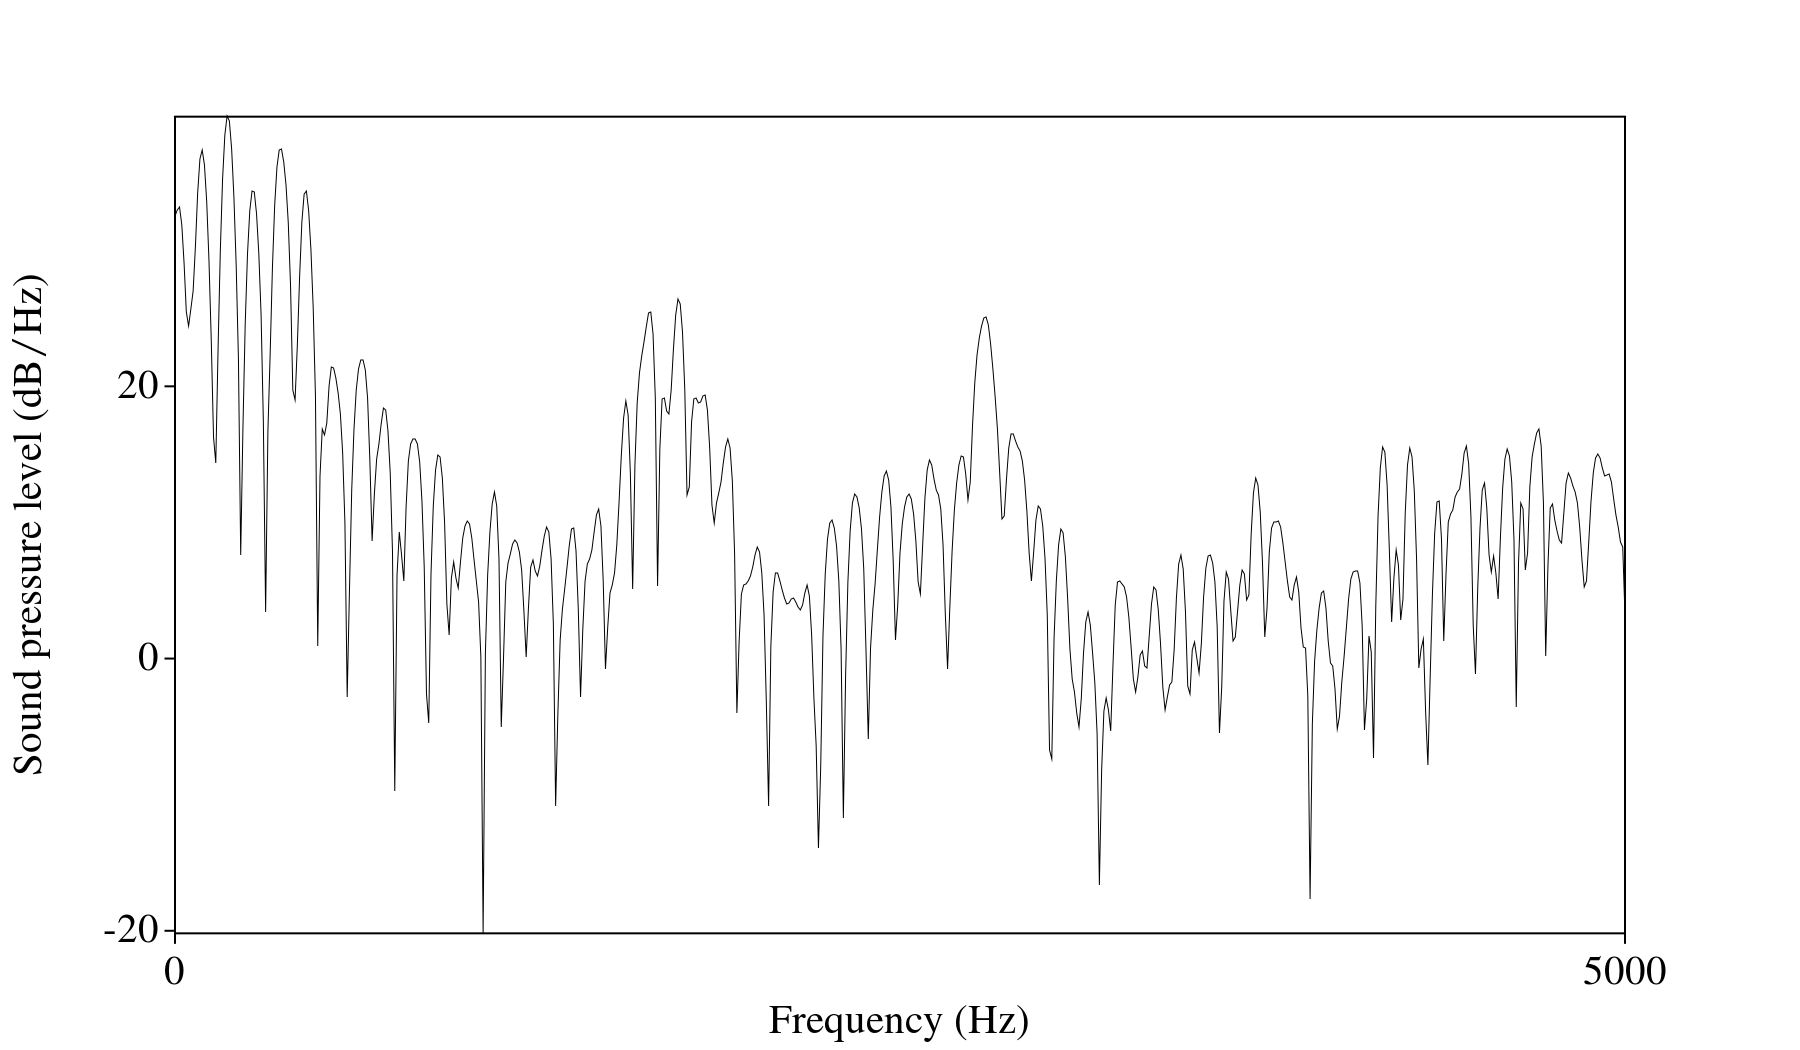
\includegraphics[width=0.5\textwidth]{figure/spctrm5k.png}
  \caption{Spectrum of the middle of an /I/ vowel.  Each `spike' is a separate narrow band of frequency, called a harmonic.}
  \label{fig:spctrm5k}
\end{wrapfigure}
%
Certain harmonics will be dampened by the vocal tract, leaving others relatively unfiltered.  A group of neighboring harmonics containing more energy than other harmonics are called formants.  The location, shape, and transition over time of these formants (among other more minor features) are what encodes speech information for voiced sounds.  This can be easily visualized in a spectrogram (cf. Fig. \ref{fig:spctgrm_citizen}).

\begin{figure}[h!]
\begin{subfigure}{0.95\textwidth}
  \centering
  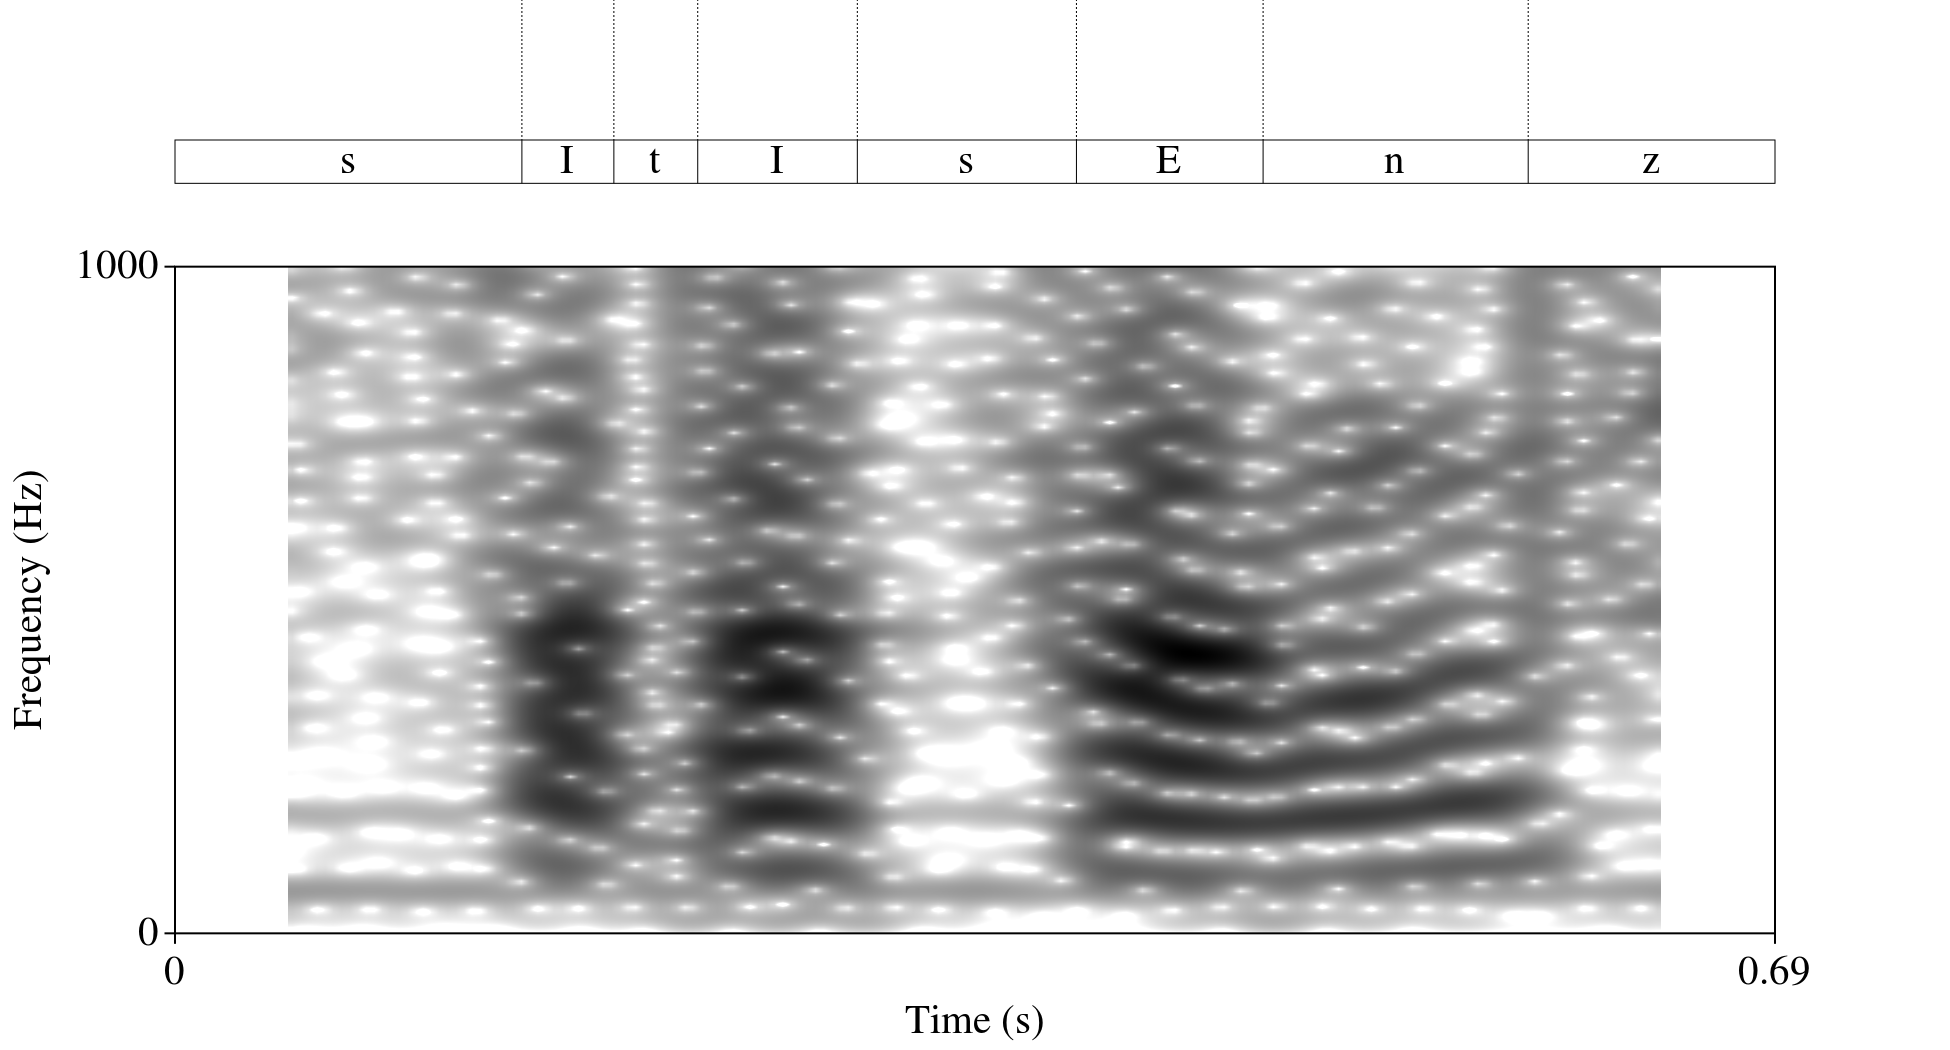
\includegraphics[width=0.95\textwidth]{figure/spctgrm1k.png}
  \caption{Zoomed to the 0-1kHz range for better visualization of harmonics.}
  \label{fig:spctgrm_citizen_1k}
\end{subfigure}%
\hfill
\begin{subfigure}{0.95\textwidth}
  \centering
  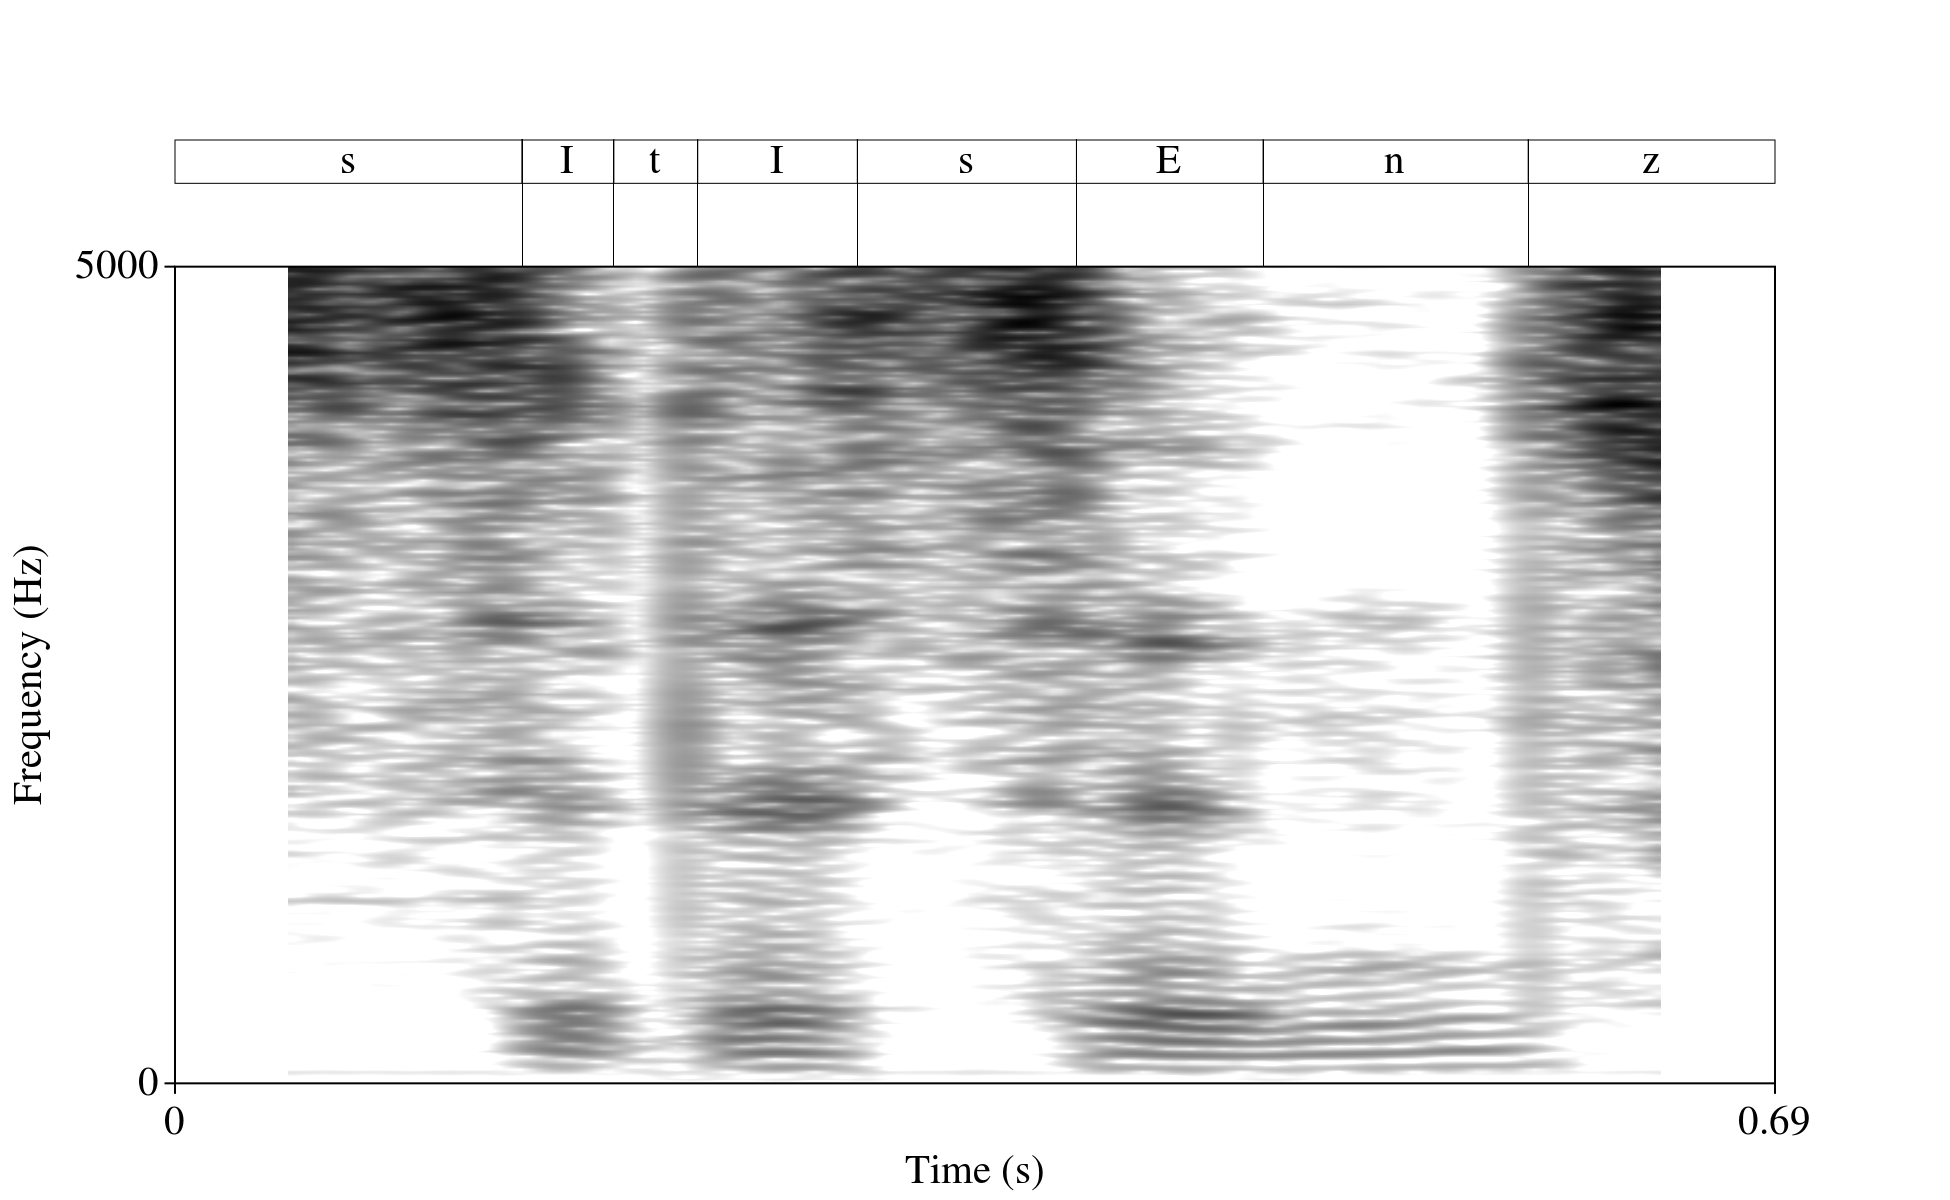
\includegraphics[width=0.95\textwidth]{figure/spctgrm5k.png}
  \caption{Zoomed to a more standard 0-5kHz range.}
  \label{fig:spctgrm_citizen_5k}
\end{subfigure}
\caption{Spectrogram of the word `citizens' with phonetic transcription above.  Frequency is on the y-axis, time is on the x-axis, and amplitude is shown in grayscale on the graph; the darker an area of the graph, the greater the amplitude.}
\label{fig:spctgrm_citizen}
\end{figure}

For unvoiced speech, the information used to recognize and categorize the speech sound is likely found in either the turbulent frication generally centered in higher frequencies (cf. Fig. \ref{fig:spctgrm_s}, although some of the information can be found in lower frequencies), or found in the voiced information in the transitions into and out of the sound (\cite{willi:17}).
%
\begin{wrapfigure}{l}{0.5\textwidth}
\centering
  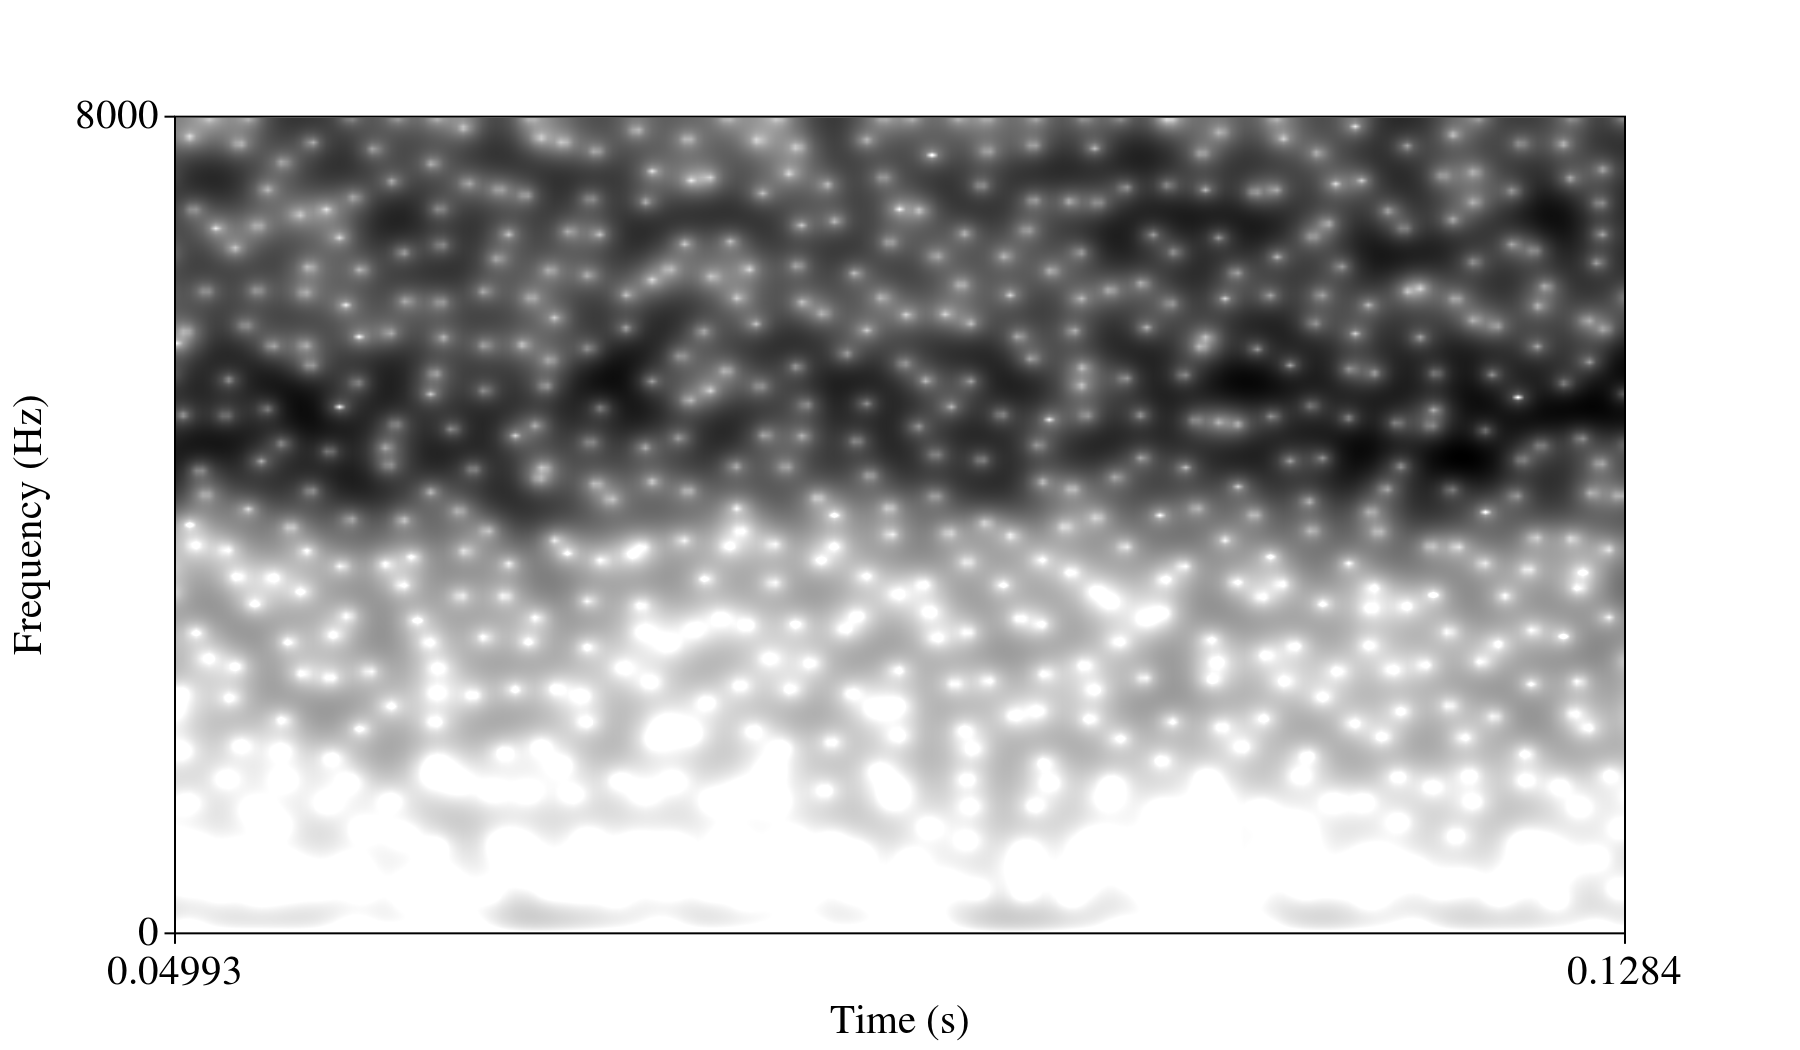
\includegraphics[width=0.5\textwidth]{figure/spctgrm_s.png}
  \caption{Spectrum of the initial /s/ in `citizens'. Zoomed to range of 0-8kHz for visualization of high frequency energy.}
  \label{fig:spctgrm_s}
\end{wrapfigure}

The human auditory system has the remarkable ability to (a) identify these sounds, which often only last from tens to a few hundreds of milliseconds in duration, (b) partition the stream of sounds into their respective words, and (c) string the words together into a sentence and pull meaning from it - all in real time.  Nevertheless there are occasionally recognition errors, which can occur anywhere along this auditory chain.  The `lowest' level in this chain that errors occur is the recognition and identification of sounds.  There are a host of reasons why this might occur, yet this report will focus on one of them - additive noise interfering with the speech signal.

\subsection{Acoustics of Multiple Signals}

As previously mentioned, we as humans use the amplitude and frequency of pressure fluctuations to perceive sound. When sound travels through a medium from source \textit{A}, there is nothing that prevents these pressure fluctuations of source \textit{A} from acoustically mixing with the pressure fluctuations originating from source \textit{B}.  For example, in Figure \ref{fig:sound-wave-addition} source \textit{A} produces a simple wave with a frequency of 100 Hz.  Source \textit{B} produces a simple wave with a frequency of 200 Hz.  If the waves from the two sources reach each other and overlap, a single wave results that looks like that in Figure \ref{fig:sound-wave-addition-combined}.  This sound wave now has two components - a tone at 100 Hz and a tone at 200 Hz.

\begin{figure}[h!]
\begin{subfigure}{0.5\textwidth}
  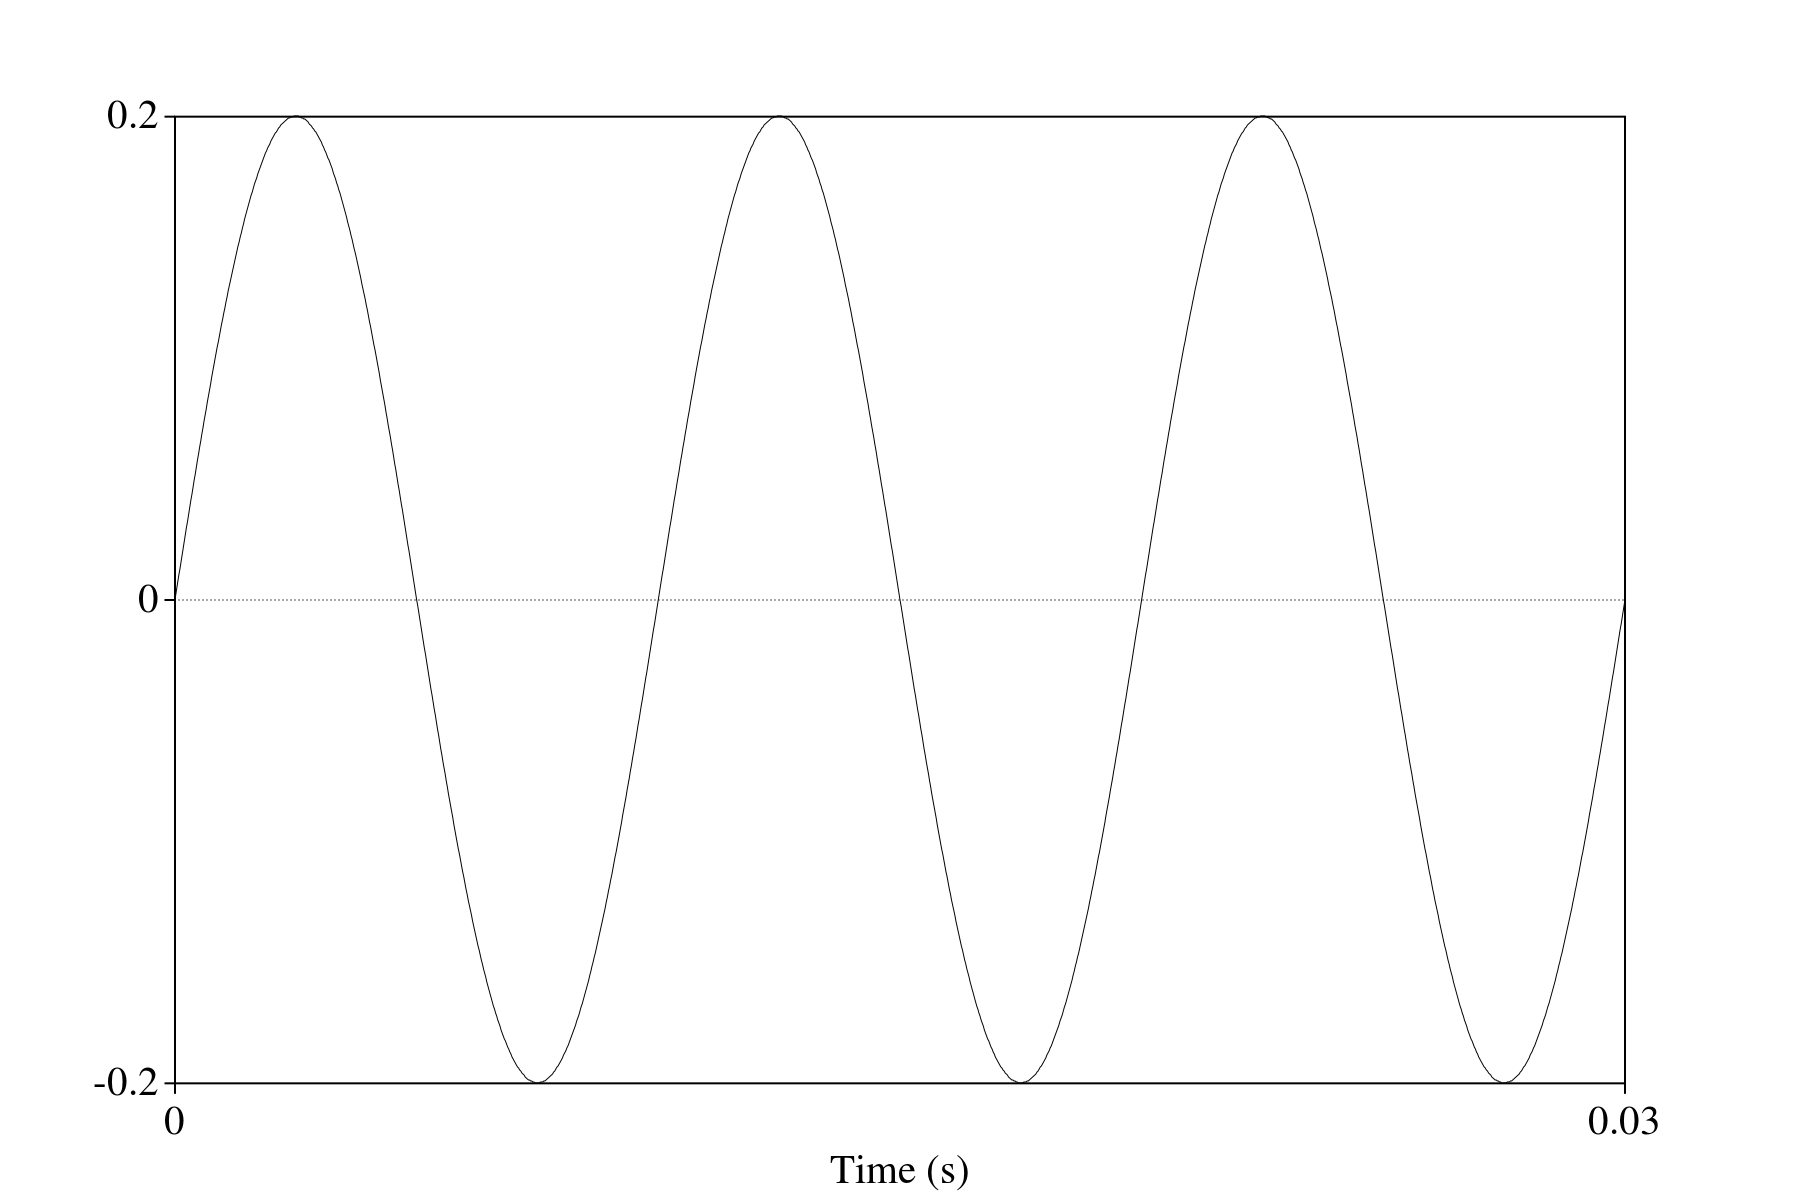
\includegraphics[width=\textwidth]{figure/basic-sound-wave.png}
  \caption{A basic sound wave from source \textit{A} at a frequency of 100 Hz.}
  \label{fig:sound-wave-A}
\end{subfigure}
\qquad
\begin{subfigure}{0.5\textwidth}
  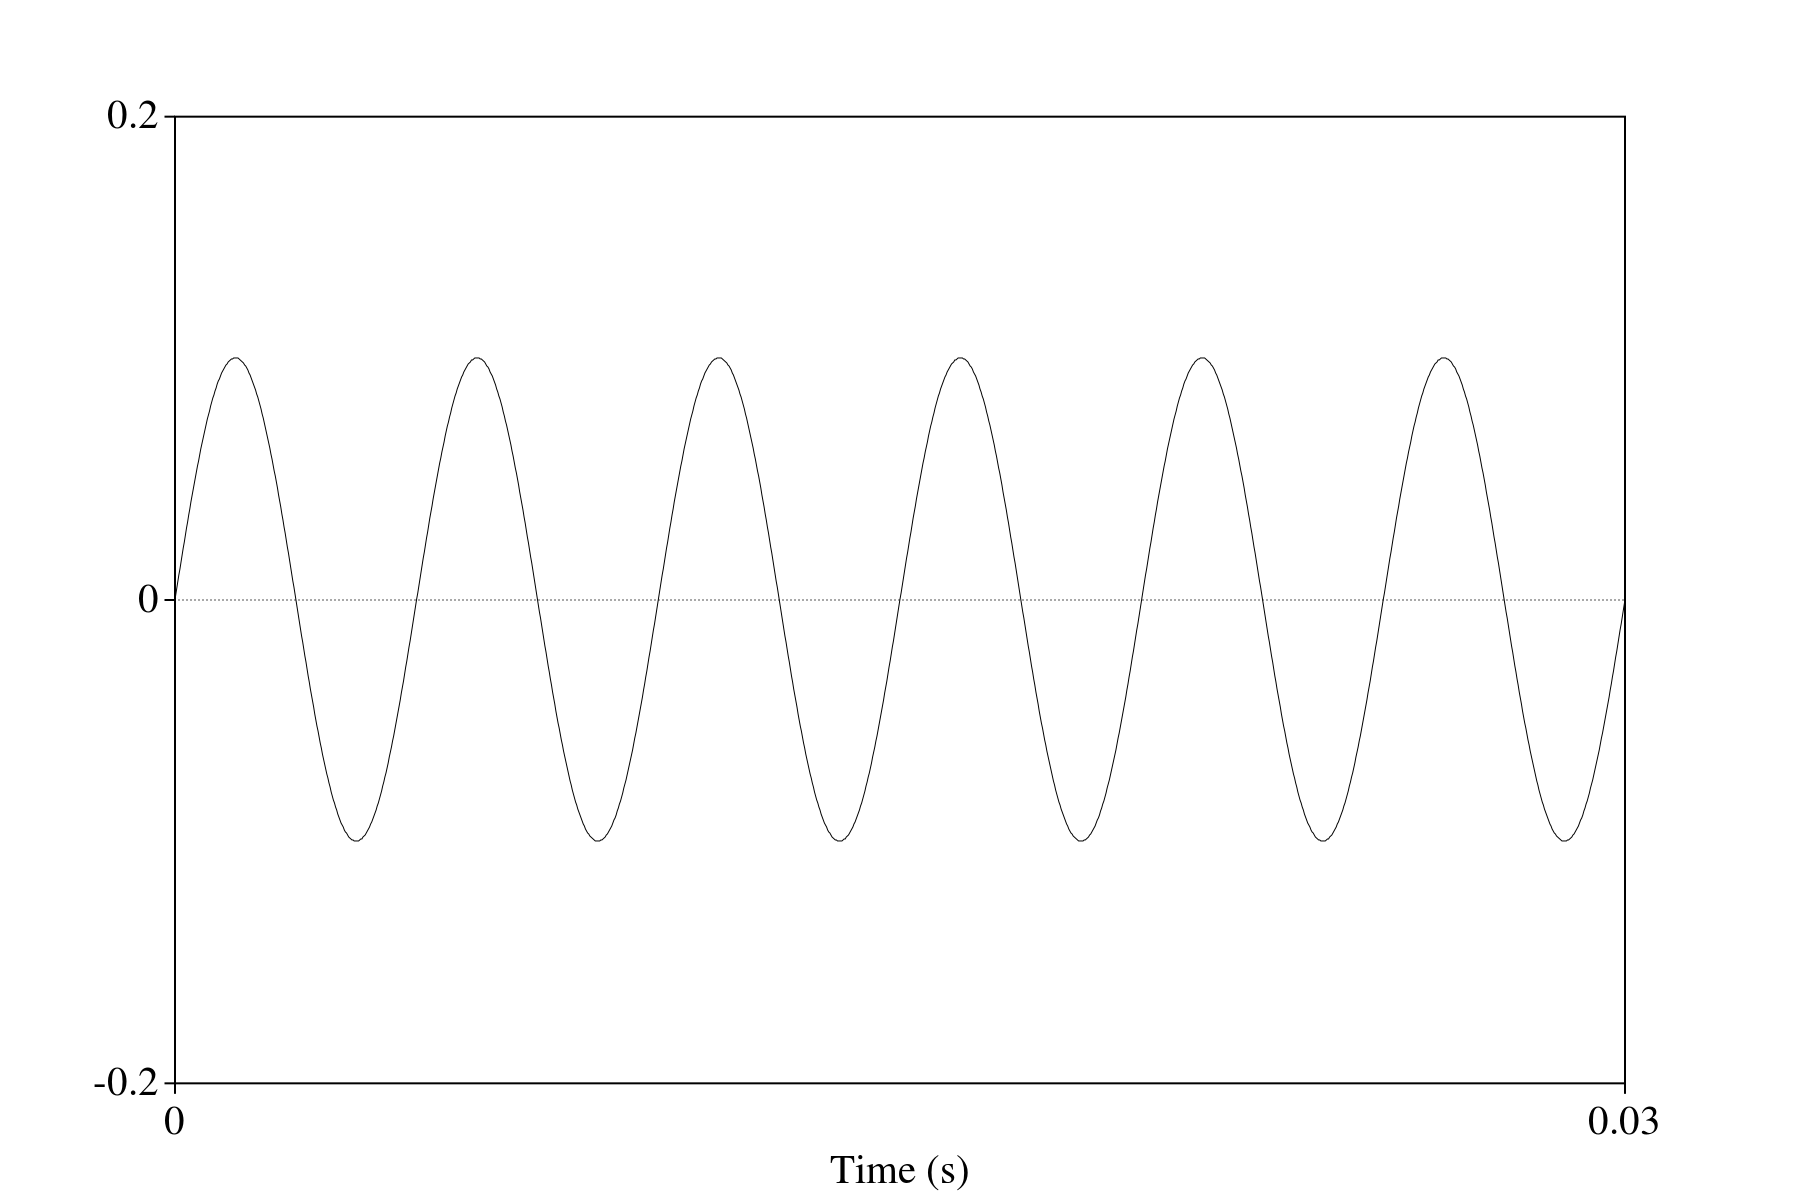
\includegraphics[width=\textwidth]{figure/sound-wave-addition-200hz.png}
  \caption{A basic sound wave from source \textit{B} at a frequency of 200 Hz, with half the amplitude of the simple sound wave from source \textit{A}.}
  \label{fig:sound-wave-B}
\end{subfigure}
%
\\[2ex]
\begin{center}
\begin{subfigure}{0.5\textwidth}
  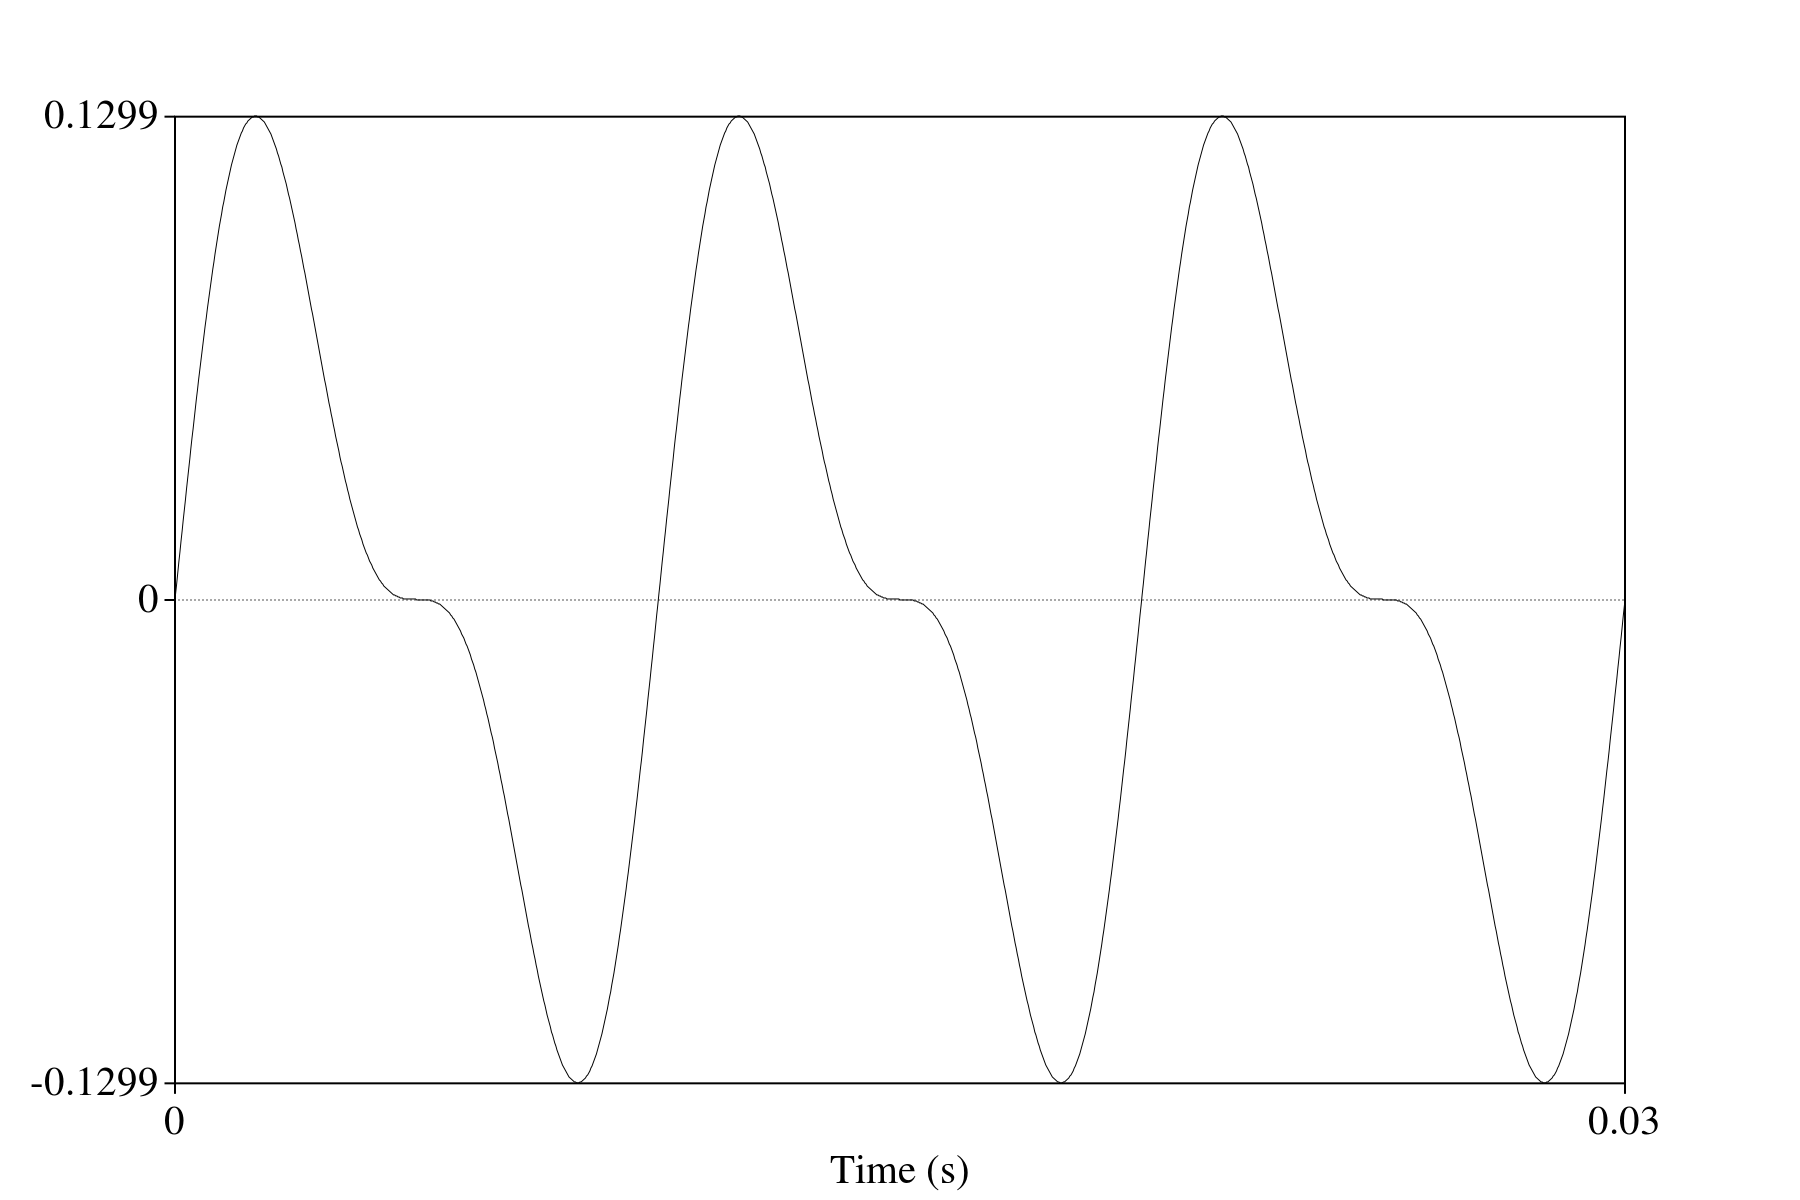
\includegraphics[width=\textwidth]{figure/sound-wave-addition-combined.png}
  \caption{The resulting complex wave from the combination of the wave from source \textit{A} and source \textit{B}.}
  \label{fig:sound-wave-addition-combined}
\end{subfigure}
\end{center}
\caption{Demonstration of the combination of two waves of different frequency and amplitude.}
\label{fig:sound-wave-addition}
\end{figure}

As previously mentioned, phase does not play a significant role in human audition, but can affect a wave resulting from the addition of multiple sound sources.  Say that source \textit{B} produces instead a wave the same frequency and amplitude as the wave from source \textit{A}, but they are completely `out of phase', ie. the pressure value of the waves at any given time is in direct opposition (cf. Figure \ref{fig:wave-out-of-phase}).  If these waves are combined, it results in a complete elimination of sound (cf. Fig. \ref{fig:wave-out-of-phase-added}).

\begin{figure}[h!]
\begin{subfigure}{0.5\textwidth}
  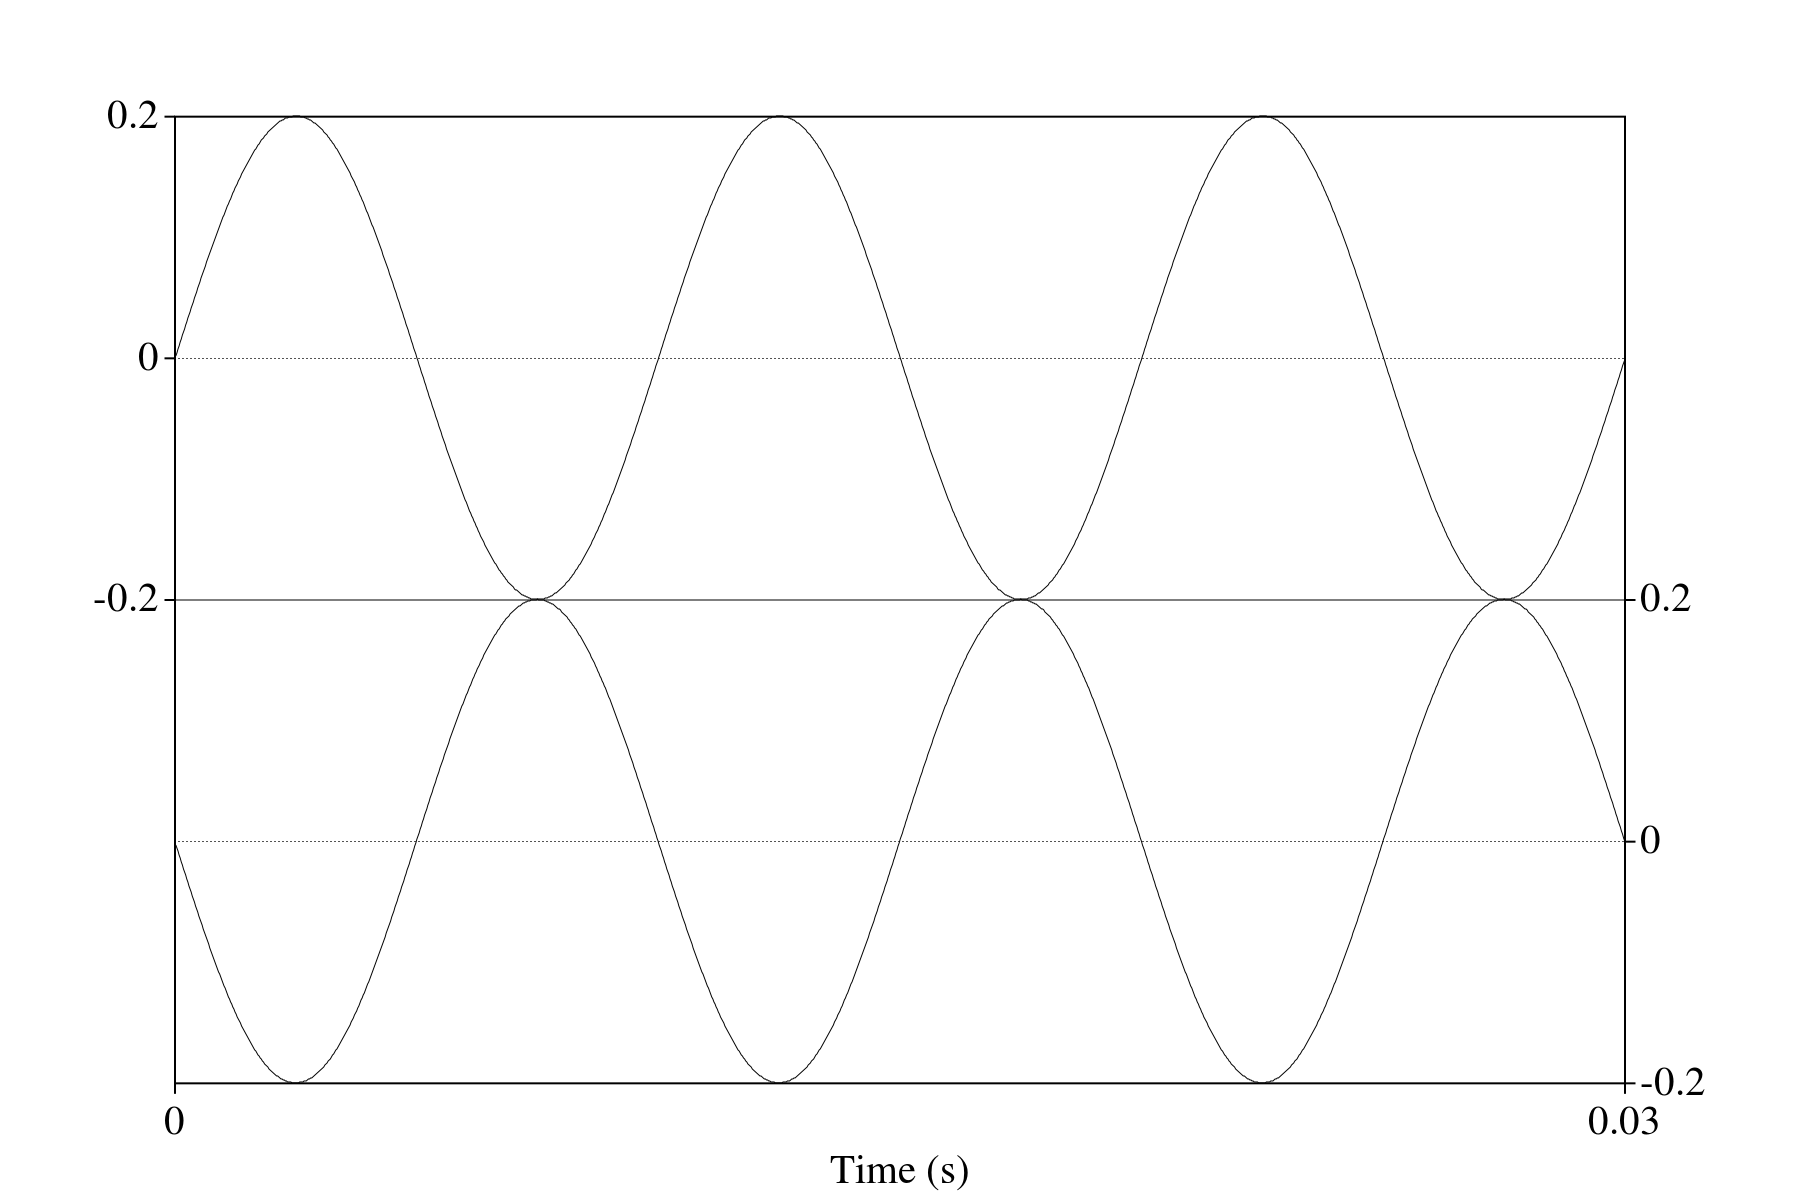
\includegraphics[width=\textwidth]{figure/wave-out-of-phase.png}
  \caption{Two sound waves with frequency of 100 Hz and the same amplitude, completely out of phase.}
  \label{fig:wave-out-of-phase}
\end{subfigure}
\qquad
\begin{subfigure}{0.5\textwidth}
  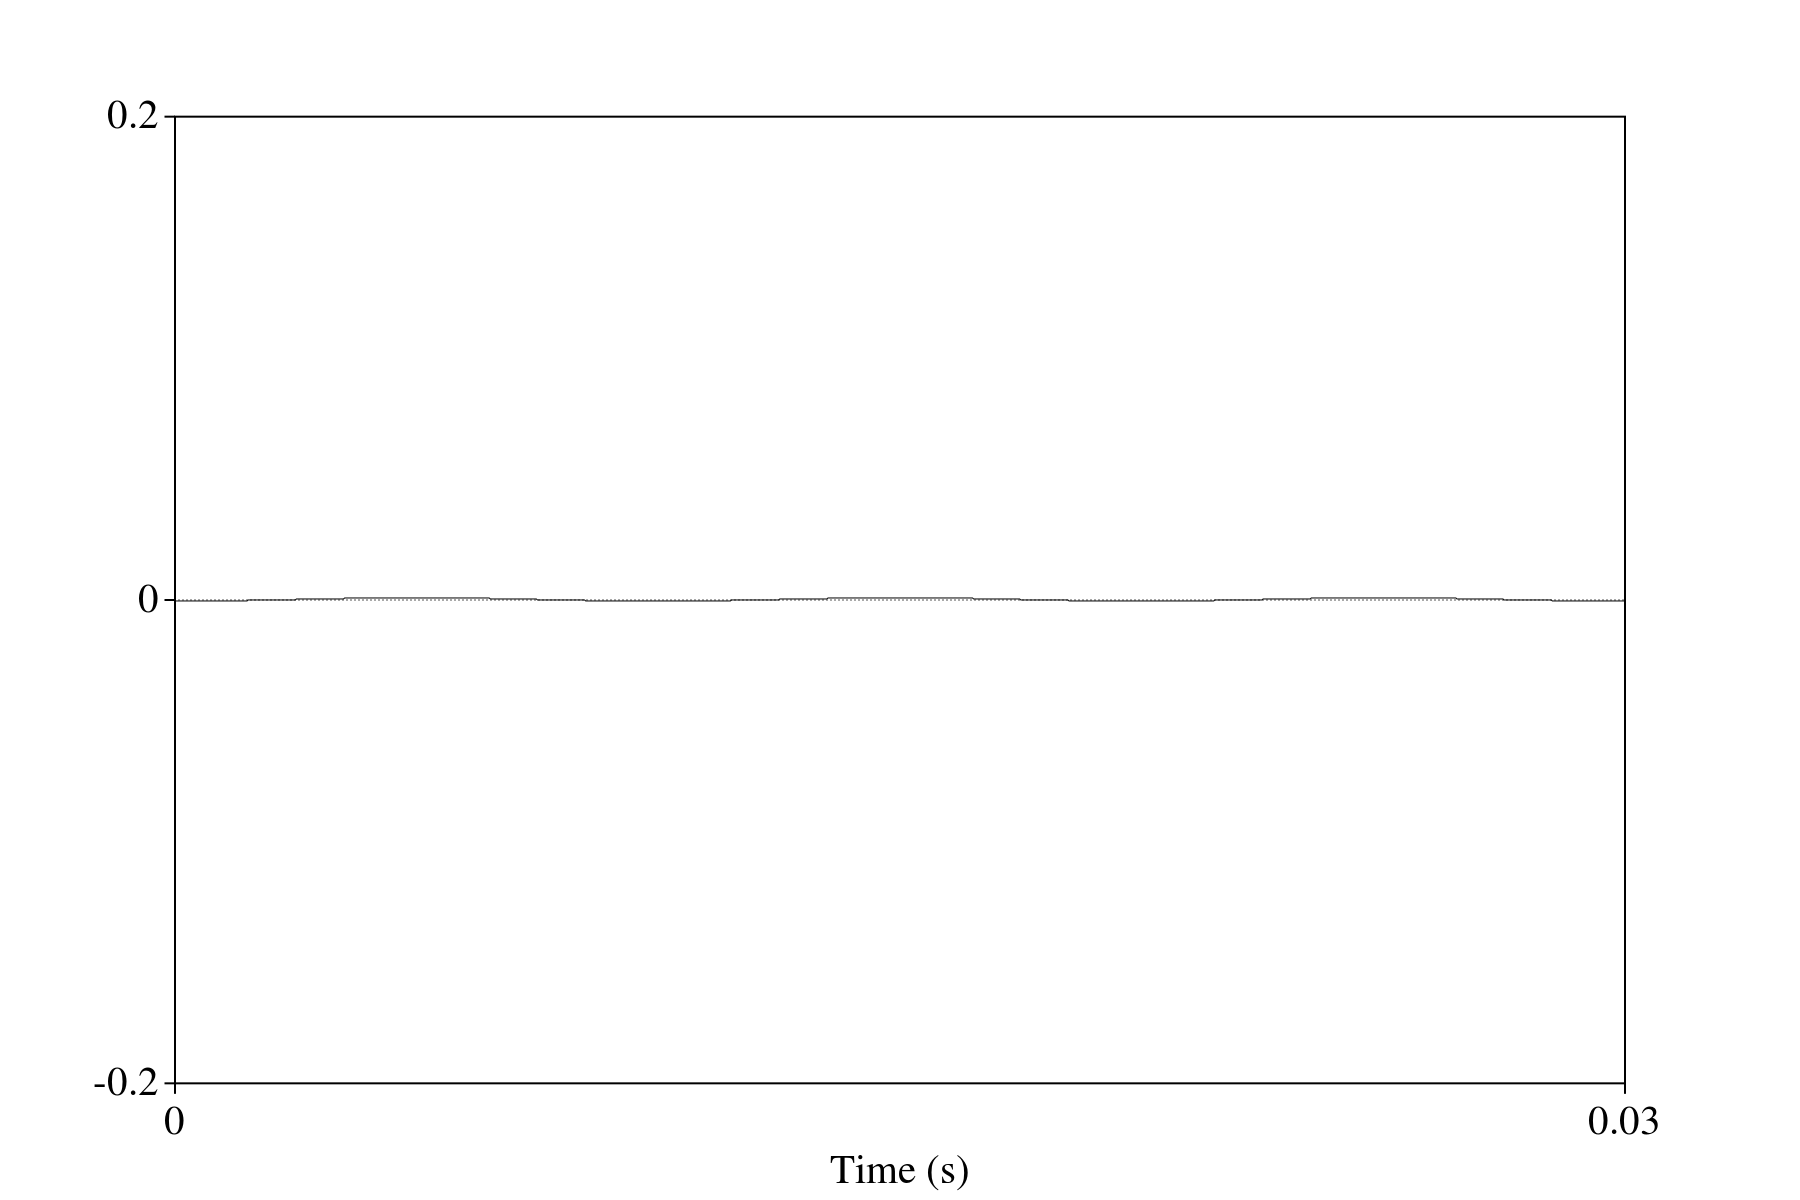
\includegraphics[width=\textwidth]{figure/wave-out-of-phase-added.png}
  \caption{The sound wave resulting from the combination of the two out of phase waves in Fig. \ref{fig:wave-out-of-phase}.}
  \label{fig:wave-out-of-phase-added}
\end{subfigure}
\caption{Demonstration of the combination of two completely out-of-phase waves with the same amplitude and frequency.}
\end{figure}

In order for this complete negation to happen, the two waves need to be coming from opposite directions toward one another.  Of course, it is not very often that two waves of the exact same frequency and amplitude, with exactly opposing phase, meet in such a way to completely negate.  However, varying degrees of negation occur frequently due to phase.  For example, if the 100 Hz wave from Figure \ref{fig:sound-wave-addition} were combined with a 200Hz wave with a slightly shifted phase, a different wave would be produced, seen in Figure \ref{fig:sound-combined-shifted-phase}.  

\begin{figure}[h!]
\begin{subfigure}{0.5\textwidth}
  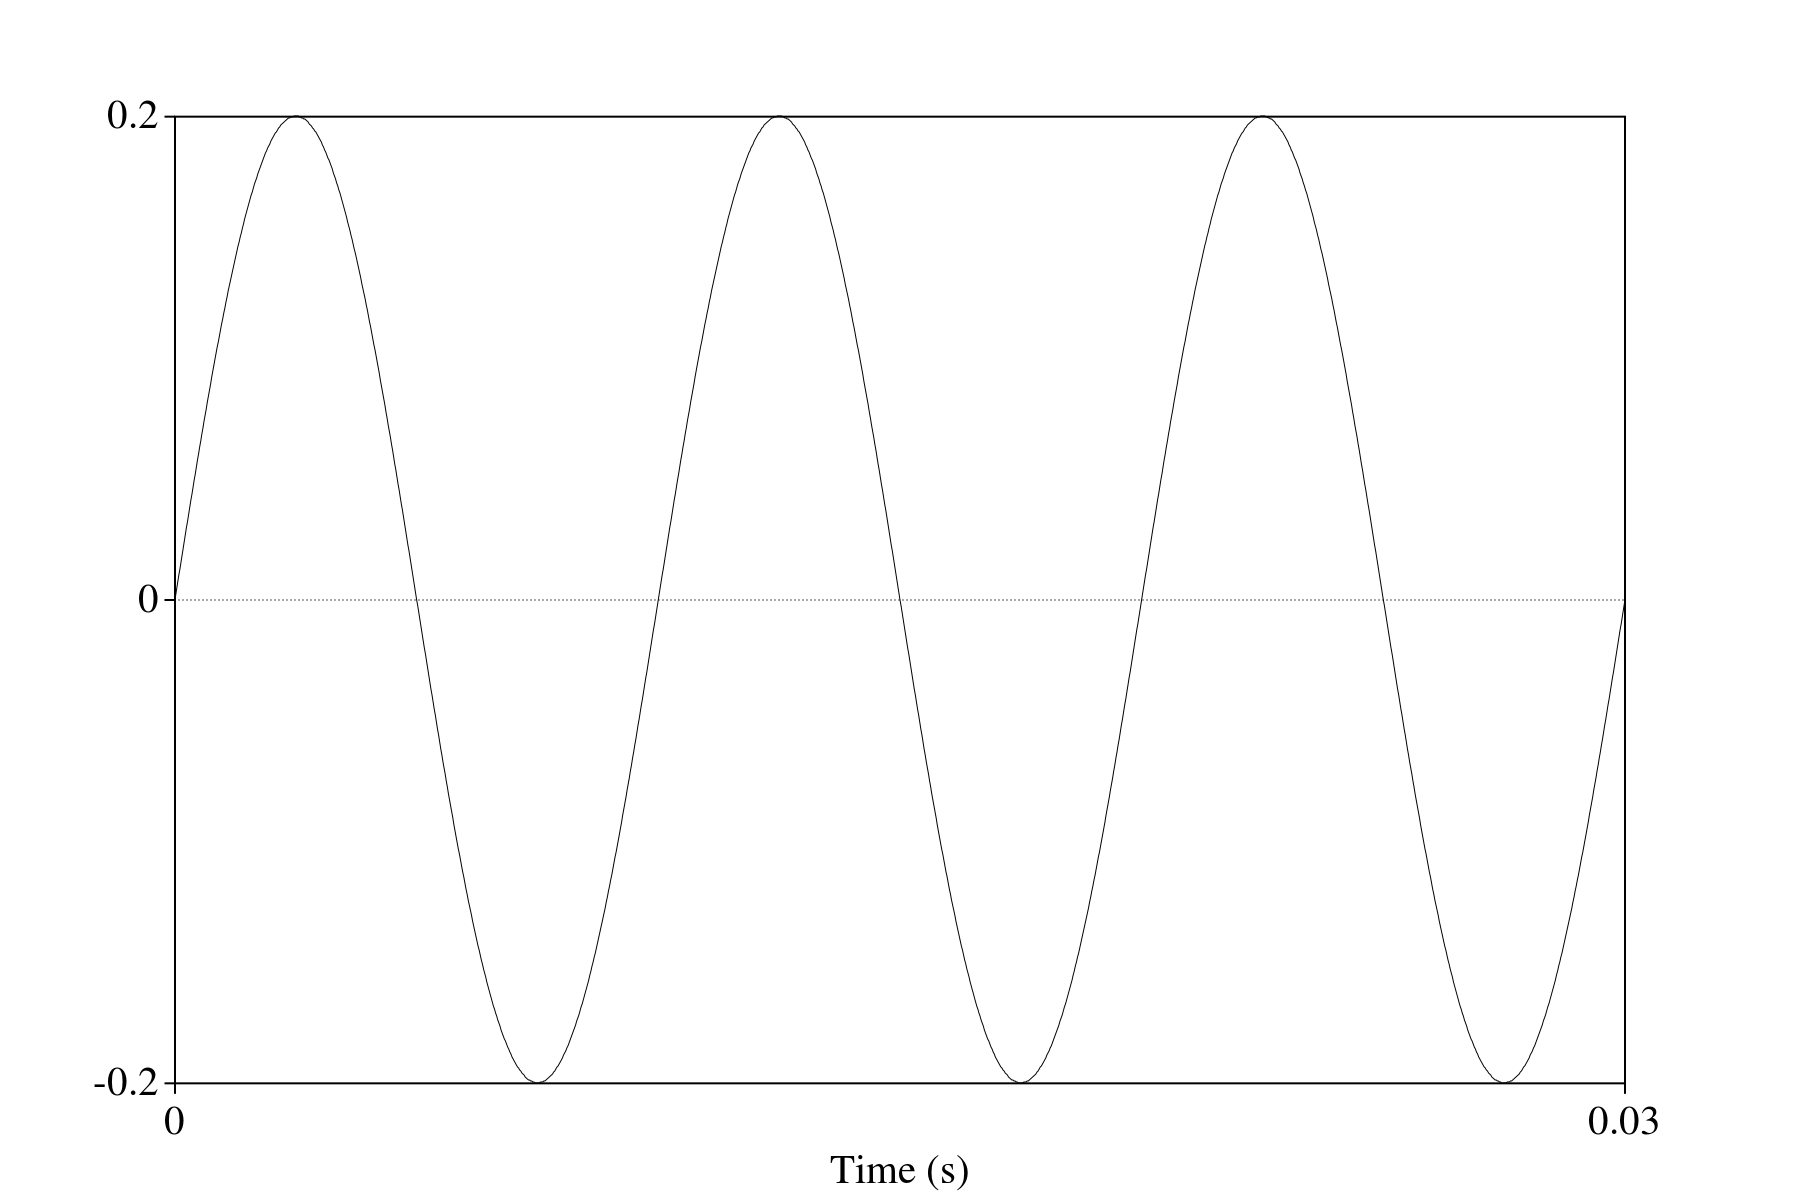
\includegraphics[width=\textwidth]{figure/basic-sound-wave.png}
  \caption{Two sound waves with frequency of 100 Hz and the same amplitude, completely out of phase.}
  \label{fig:wave-out-of-phase}
\end{subfigure}
\qquad
\begin{subfigure}{0.5\textwidth}
  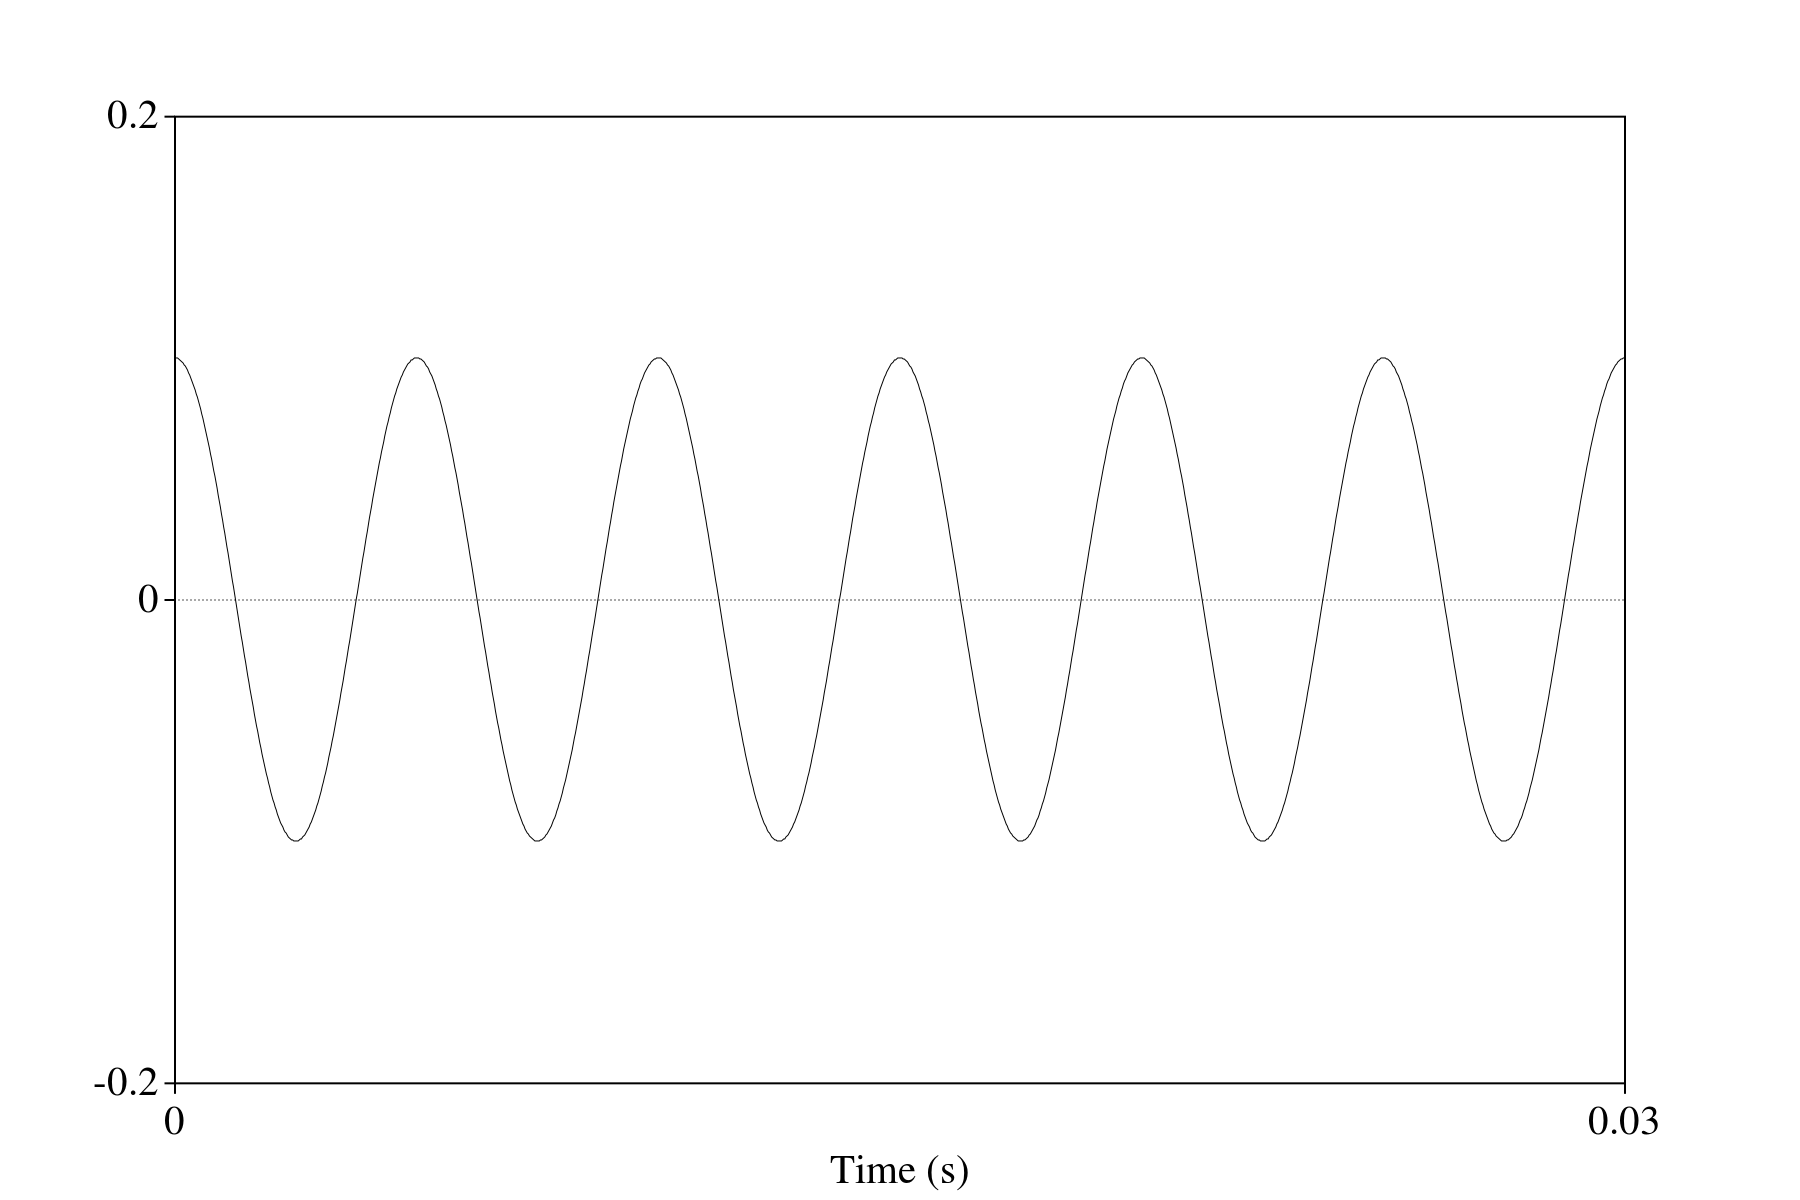
\includegraphics[width=\textwidth]{figure/sound-wave-addition-200hz-shifted.png}
  \caption{The sound wave resulting from the combination of the two out of phase waves in Fig. \ref{fig:wave-out-of-phase}.}
  \label{fig:wave-addition-200hz-shifted}
\end{subfigure}
%
\begin{center}
\begin{subfigure}{0.5\textwidth}
  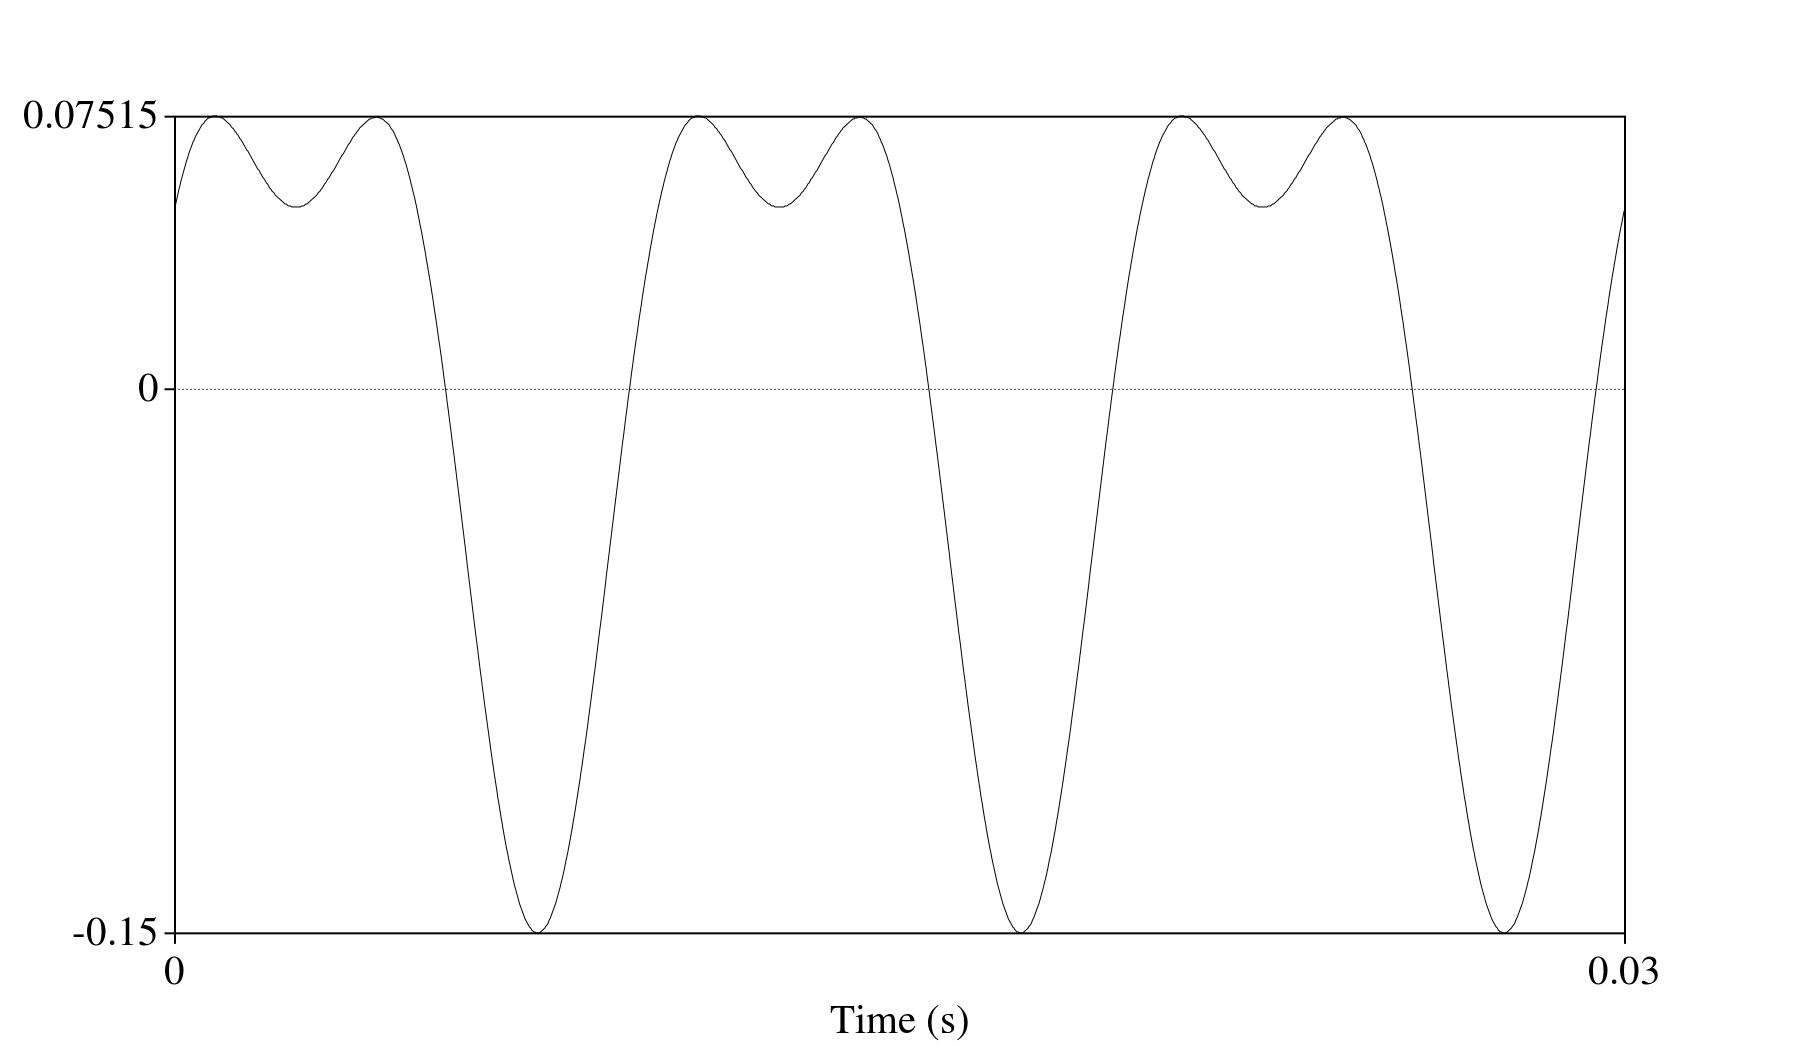
\includegraphics[width=\textwidth]{figure/sound-combined-shifted-phase.png}
  \caption{The sound wave resulting from the combination of the two out of phase waves in Fig. \ref{fig:wave-out-of-phase}.}
  \label{fig:sound-combined-shifted-phase}
\end{subfigure}
\end{center}
\caption{Demonstration of the combination of the same two waves as in Fig. \ref{fig:sound-wave-addition}, where the phase of the 200 Hz wave in Fig. \ref{fig:sound-wave-B} was shifted slightly (cf. Fig. \ref{fig:wave-addition-200hz-shifted})}
\label{fig:sound-shifted-phase}
\end{figure}

The combination of waves from multiple sound sources increases greatly in complexity as the number of sources increases, and the sounds originating from the sources are complex (ie. containing multiple frequency elements), such as speech.  Speech rarely occurs in isolation from from all external sound, yet we are still to largely understand speech in everyday environments; for example it is generally easy for humans to understand the speech of an interlocutor while sitting on a bench at a park.

The auditory system is actually quite skilled at identifying separate sources, even complex ones, like speech. Despite the shifted phase in Figure \ref{fig:sound-shifted-phase}, the human auditory system would still be able to detect and identify two separate waves.  While it undoubtedly plays a part, the differences in phase of combined signals does not normally completely negate a signal, nor render it unintelligible.  It is for this reason, and the complexity of phase calculations, that most efforts to remove speech from noise ignore the phase component.

\subsection{Difficulties of Speech in Noise}

Nevertheless, there are still situations in which it is difficult to parse speech in noise.  This is most often due to signals with energy at similar frequencies that overlap.  The greater the amplitude of a signal at frequencies overlapping with those of speech, the more difficult the speech will be to understand.  This can be visualized in the spectrograms of the sentence ``A rich farm is rare in this sandy waste.'' in Figure \ref{fig:signal-SNR-intro}.  In Figure \ref{fig:signal-SNR-intro-high}, the amplitude, or loudness, of the noise is well below that of speech, which would likely be easily understand by a listener.  Figure \ref{fig:signal-SNR-intro-low} has a much greater noise amplitude level compared to the amplitude level of speech and consequently would likely be more difficult for a listener to understand.

\begin{figure}[h!]
\centering
\begin{subfigure}{0.75\textwidth}
  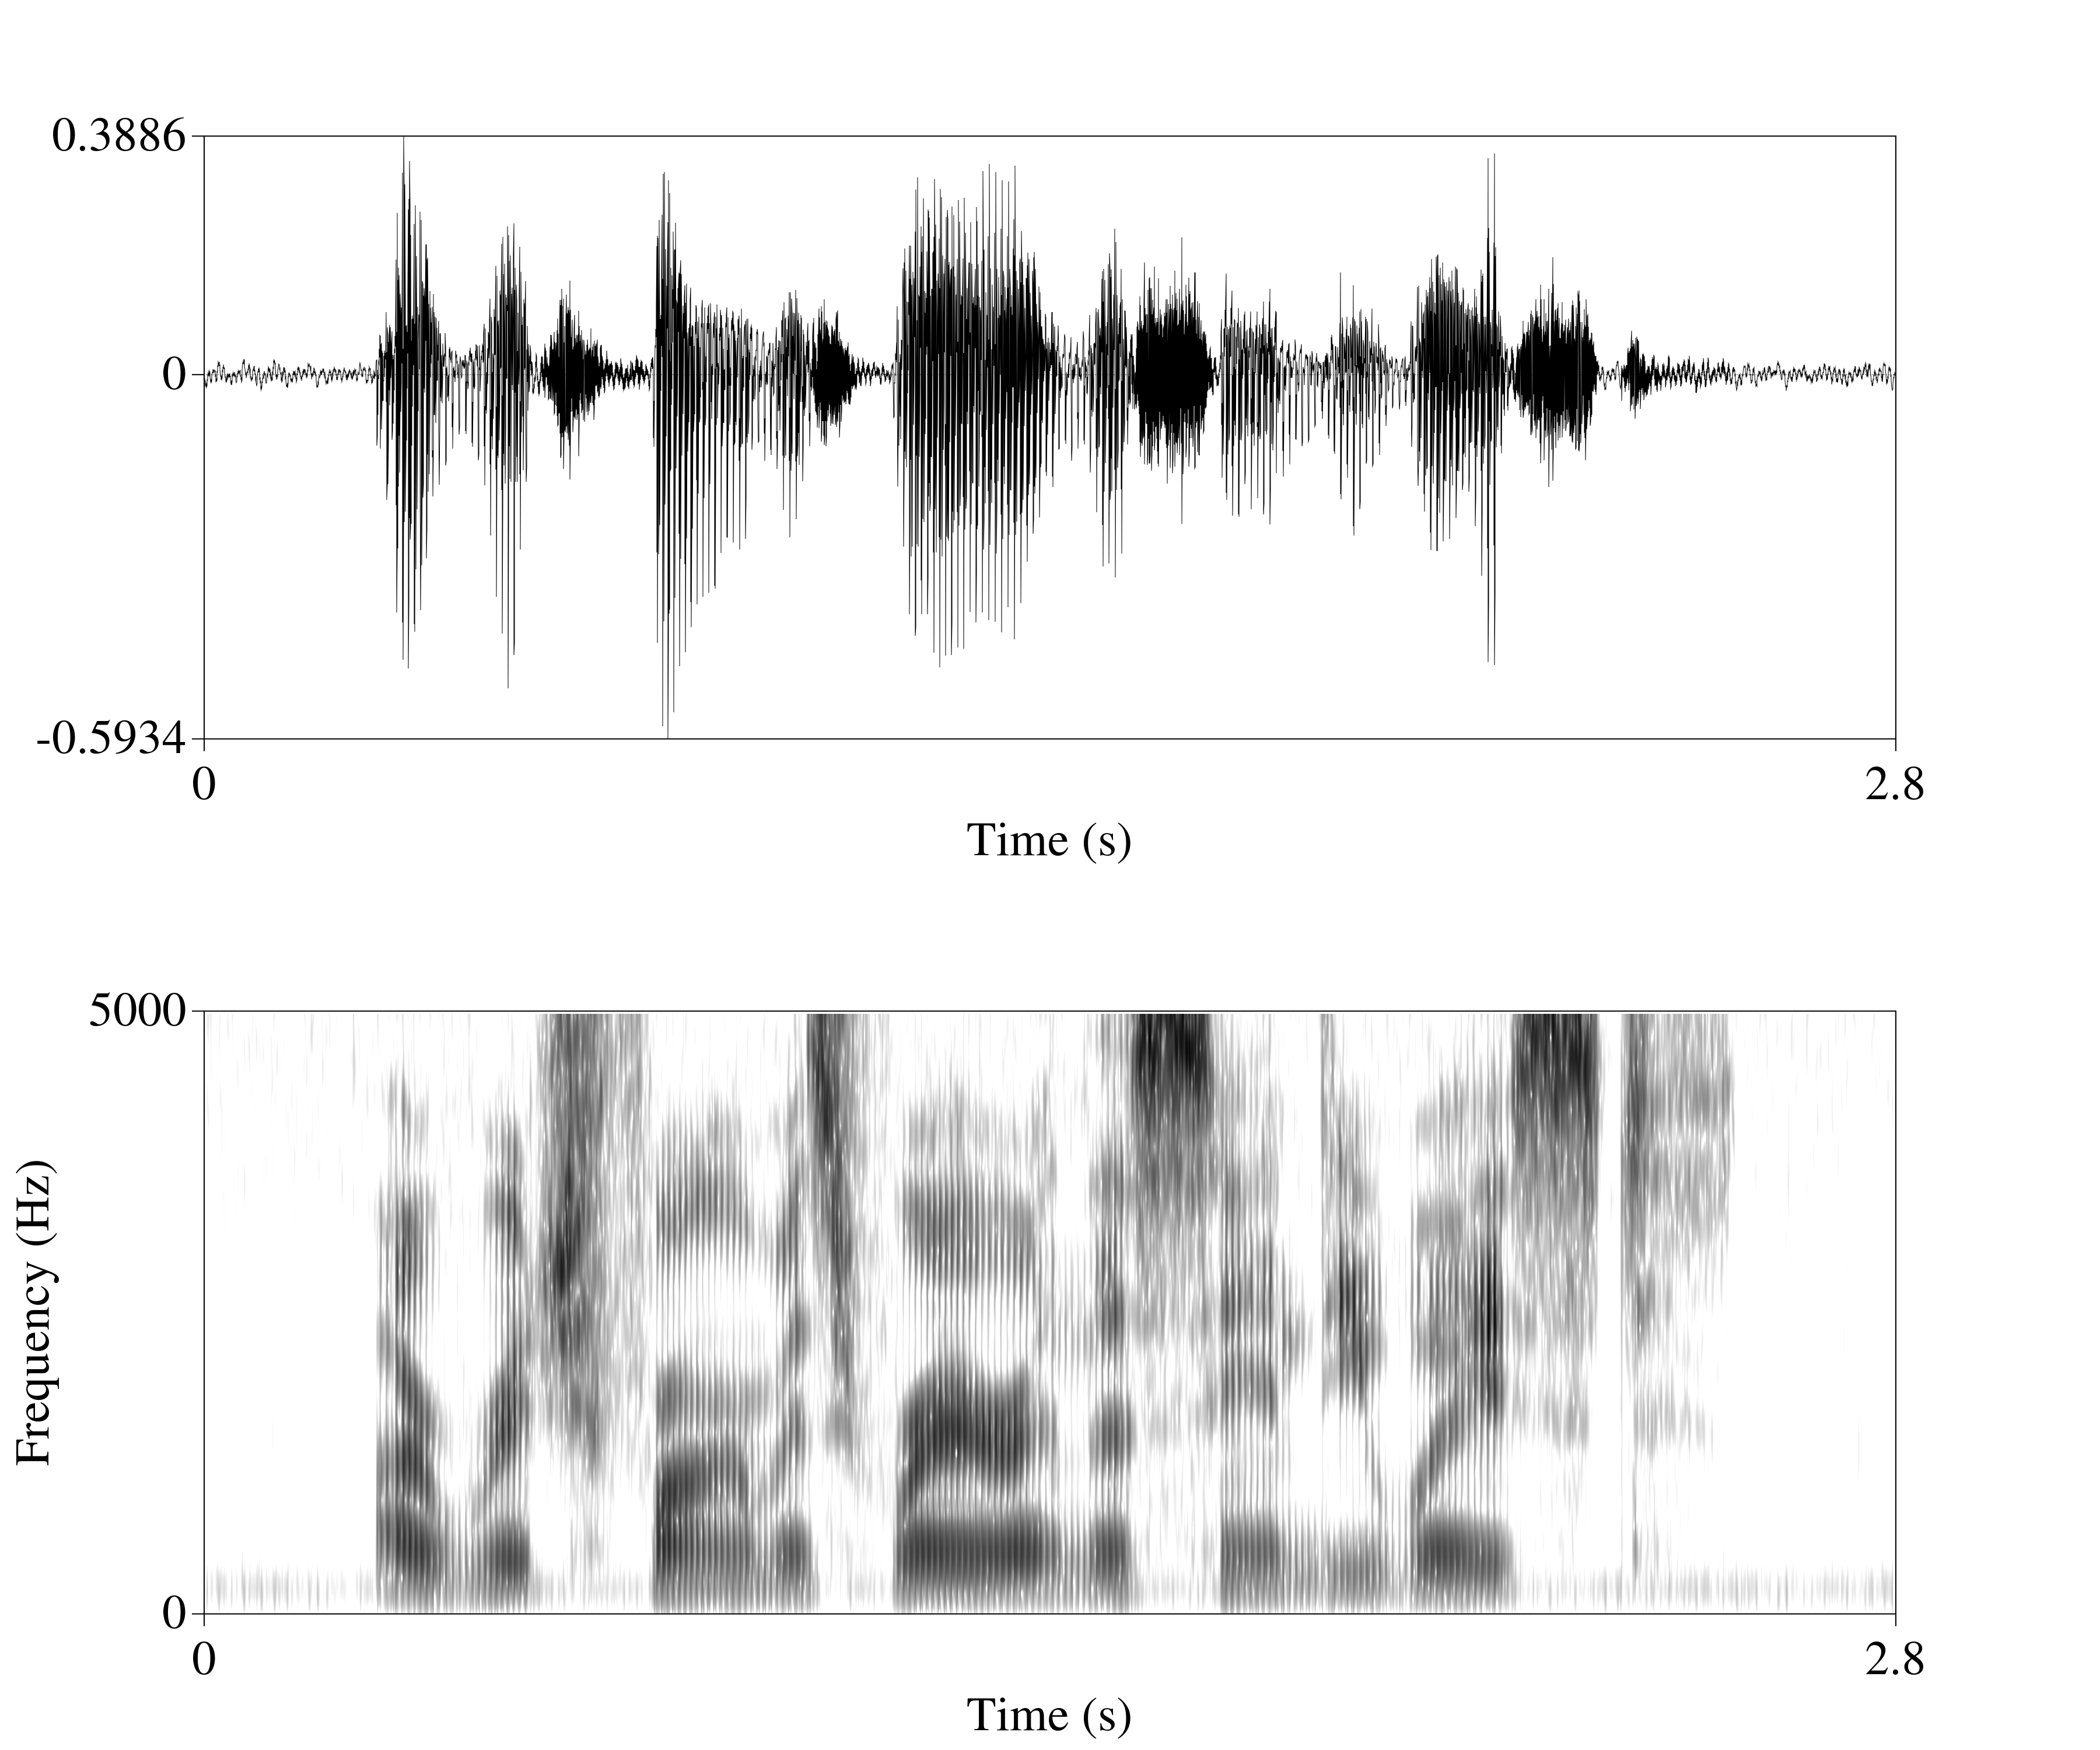
\includegraphics[width=.9\textwidth]{figure/signal-SNR-intro-high.png}
  \caption{A sentence spoken with a low level of background noise, resulting in a \textit{high} SNR.}
  \label{fig:signal-SNR-intro-high}
\end{subfigure}
%
\begin{subfigure}{0.75\textwidth}
  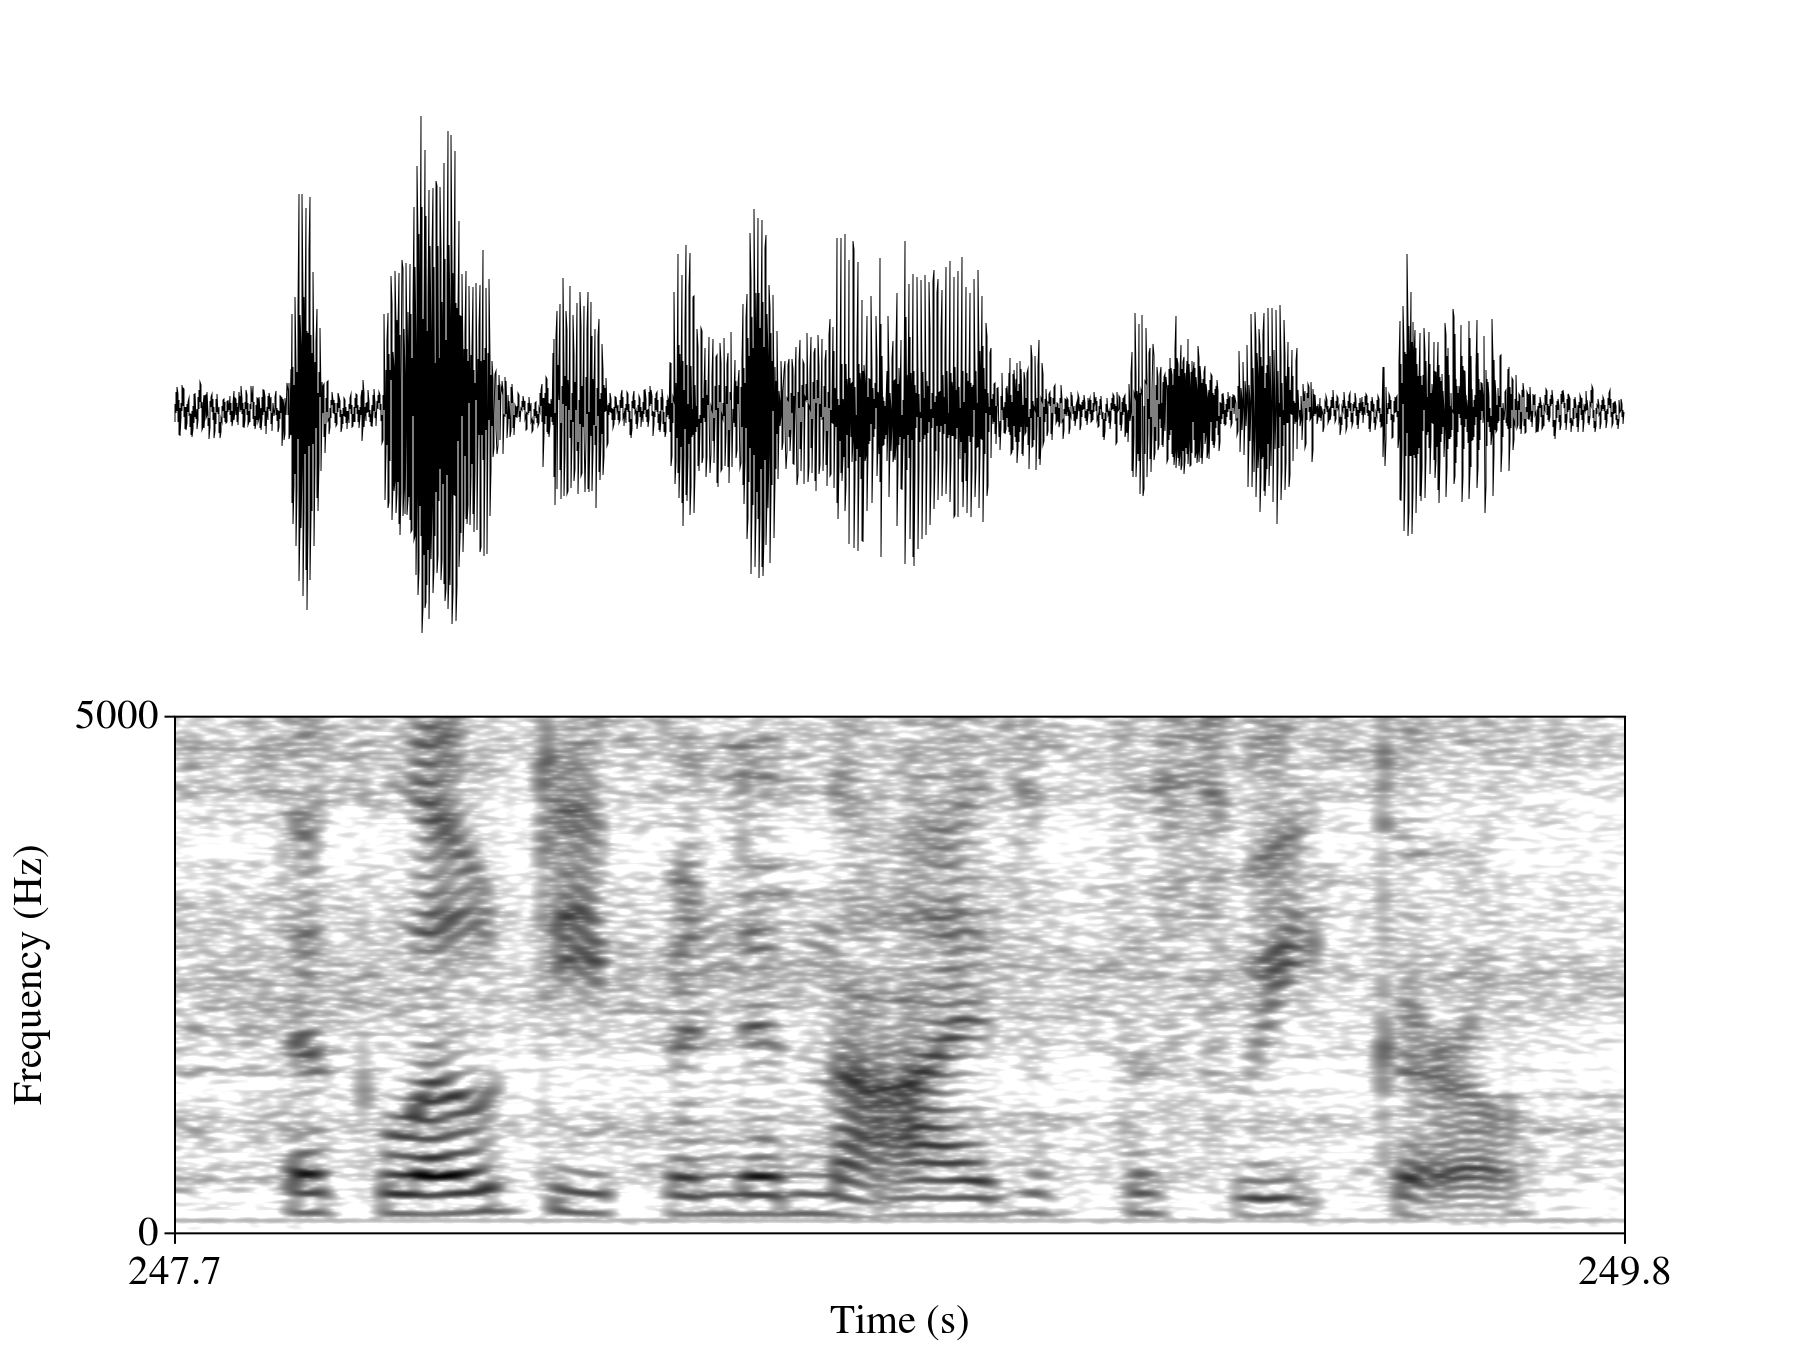
\includegraphics[width=.9\textwidth]{figure/signal-SNR-intro-low.png}
  \caption{A sentence spoken with a high level of background noise, resulting in a \textit{low} SNR.}
  \label{fig:signal-SNR-intro-low}
\end{subfigure}
\caption{Waveforms and spectrograms of the sentence ``A rich farm is rare in this sandy waste''.}
\label{fig:signal-SNR-intro}
\end{figure}

This relationship between speech and any background noise is called the signal to noise ration (SNR).  A complex signal with a higher signal to noise ratio (cf. Fig \ref{fig:signal-SNR-intro-high}) is generally easier to understand, because the amplitude of the speech (the `signal' of interest) is much greater than that of the noise.  Consequently a lower SNR (cf. Fig. \ref{fig:signal-SNR-intro-low}) results in speech that is more difficult to understand, because the amplitude of the speech is close to - or below - the amplitude of the background noise.

This poses a problem for human listeners, but generally is more difficult to deal with in automatic speech recognition (ASR), since the electronic device does not contain a highly-skilled, built-in auditory cortex.  There are a number of ways which have been proposed to deal with noise in a speech signal, both for human and automatic speech recognition.  These will be discussed further in Chapters \ref{chapter3} and \ref{chapter4}.

\section{Overview of Dissertation}\label{ch1:diss-overview}

This report aims to explore a novel method of human speech perception and automatic speech recognition (ASR) in noisy environments.  The method proposes that speech be recorded from the inside of the ear canal of the speaker, slightly transformed, and sent to the human listener or the computer receiver for recognition.  Collecting speech from the ear allows for usage of the human skull and adjacent tissues to passively filter out the noisy environment, leaving only - or mostly - the human speech carrying the intended message.  
	
The intention of this study is to determine a) if recording human speech from the inside of the ear canal can significantly reduce background noise in a signal, b) if intelligible speech, suitable for communication, can be collected from the inside of the ear canal, c) if humans find speech recorded from the ear canal more intelligible than speech in noisy conditions, and finally d) if ASR systems are able to recognize speech recorded in the ear canal with greater accuracy than speech recorded in noise.
	
Since currently there is no established corpus of data that contain speech recorded from the inside of the ear canal together with speech simultaneously recorded from the mouth in noisy environments, it was necessary to record speakers in this environment and create a new corpus.  The theory behind the acoustics of recording speech from the ear canal, as well as the process for developing this corpus are described in Chapter \ref{chapter2}, along with a discussion of the recorded speech.  Chapter \ref{chapter3} will outline a human perception experiment, tasking listeners with the transcription of various sentences of speech recorded at the mouth in noise in noise, and recorded from the ear.   Chapter \ref{chapter4} describes the use of this same speech with an ASR system, and its recognition performance.  Chapter \ref{chapter5} will summarize the previous chapters and engage in an overall discussion of the implications of the results, the limitations of the present experiments and methods, and suggestions for future research direction.



\documentclass[dissertation,copyright]{uathesis}
\usepackage[]{graphicx}\usepackage[]{color}
%% maxwidth is the original width if it is less than linewidth
%% otherwise use linewidth (to make sure the graphics do not exceed the margin)
\makeatletter
\def\maxwidth{ %
  \ifdim\Gin@nat@width>\linewidth
    \linewidth
  \else
    \Gin@nat@width
  \fi
}
\makeatother

\definecolor{fgcolor}{rgb}{0.345, 0.345, 0.345}
\newcommand{\hlnum}[1]{\textcolor[rgb]{0.686,0.059,0.569}{#1}}%
\newcommand{\hlstr}[1]{\textcolor[rgb]{0.192,0.494,0.8}{#1}}%
\newcommand{\hlcom}[1]{\textcolor[rgb]{0.678,0.584,0.686}{\textit{#1}}}%
\newcommand{\hlopt}[1]{\textcolor[rgb]{0,0,0}{#1}}%
\newcommand{\hlstd}[1]{\textcolor[rgb]{0.345,0.345,0.345}{#1}}%
\newcommand{\hlkwa}[1]{\textcolor[rgb]{0.161,0.373,0.58}{\textbf{#1}}}%
\newcommand{\hlkwb}[1]{\textcolor[rgb]{0.69,0.353,0.396}{#1}}%
\newcommand{\hlkwc}[1]{\textcolor[rgb]{0.333,0.667,0.333}{#1}}%
\newcommand{\hlkwd}[1]{\textcolor[rgb]{0.737,0.353,0.396}{\textbf{#1}}}%
\let\hlipl\hlkwb

\usepackage{framed}
\makeatletter
\newenvironment{kframe}{%
 \def\at@end@of@kframe{}%
 \ifinner\ifhmode%
  \def\at@end@of@kframe{\end{minipage}}%
  \begin{minipage}{\columnwidth}%
 \fi\fi%
 \def\FrameCommand##1{\hskip\@totalleftmargin \hskip-\fboxsep
 \colorbox{shadecolor}{##1}\hskip-\fboxsep
     % There is no \\@totalrightmargin, so:
     \hskip-\linewidth \hskip-\@totalleftmargin \hskip\columnwidth}%
 \MakeFramed {\advance\hsize-\width
   \@totalleftmargin\z@ \linewidth\hsize
   \@setminipage}}%
 {\par\unskip\endMakeFramed%
 \at@end@of@kframe}
\makeatother

\definecolor{shadecolor}{rgb}{.97, .97, .97}
\definecolor{messagecolor}{rgb}{0, 0, 0}
\definecolor{warningcolor}{rgb}{1, 0, 1}
\definecolor{errorcolor}{rgb}{1, 0, 0}
\newenvironment{knitrout}{}{} % an empty environment to be redefined in TeX

\usepackage{alltt}
\newcommand{\SweaveOpts}[1]{}  % do not interfere with LaTeX
\newcommand{\SweaveInput}[1]{} % because they are not real TeX commands
\newcommand{\Sexpr}[1]{}       % will only be parsed by R


%\documentclass[dissertation,CC-BY]{uathesis}
%\documentclass[dissertation,CC-BY-SA]{uathesis}
%documentclass[dissertation,CC-BY-ND]{uathesis}
%\documentclass[thesis]{uathesis}
%\documentclass[document]{uathesis}

% Package Usage
% These are the packages that we need
\usepackage{booktabs}
\usepackage{graphicx}
\usepackage{natbib}			% natbib is available on most systems, and is
					% terribly handy.
					
%May need to remove! Trying to fix nocite{*} biblography problem:
					% If you want to use a different Bibliography package, 
					% you should be able to, just change this
					% and the \bibliographystyle command below.  Be warned
					% that you may need to do a little hacking to get
					% the REFERENCES item to show up in your TOC.

% Compatibility with the AASTEX package 
% of the American Astronomical Society.
%\usepackage{deluxetable}		% Allows use of AASTEX deluxe tables
%\usepackage{aastex_hack}		% Allows other AASTEX functionality.

% These are other packages that you might find useful.
% For controlling the fonts, see
% http://www.math.uiuc.edu/~hartke/computer/latex/survey/survey.html
% The following is a nice font set:
%\usepackage{mathtime}			% Times for letters; Belleek math.
%
\usepackage{wrapfig}
\usepackage{caption}
\usepackage{subcaption}
\usepackage{tipa}
\usepackage{color,soul}
\usepackage{url}
\usepackage{blindtext}
\usepackage[inline]{enumitem}
\usepackage{breakurl}
\usepackage{mathtools}
\usepackage{amsmath}			% AMS Math (advanced math typesetting)
%\usepackage{lscape}			% Used for making fitting large tables in by putting them landscape
%\usepackage{refs}			
%
% If you are using hyper-ref (recommended), this command must go after all 
% other package inclusions (from the hyperref package documentation).
% The purpose of hyperref is to make the PDF created extensively
% cross-referenced.

%Also works! Change dvips to driverfallback=dvips.
\usepackage[driverfallback=dvips,bookmarks,colorlinks=true,urlcolor=black,linkcolor=black,citecolor=black]{hyperref}


%Works!
%\usepackage[pdftex,bookmarks,colorlinks=true,urlcolor=black,linkcolor=black,citecolor=black]{hyperref}
%HERE IS THE THING THAT NEEDS TO CHANGE TO GET LATEX TO WORK WITH RSTUDIO. USE pdftex instead of dvips.

% Set up some values.
\completetitle{Working Title: Ear Recorded Speech: A novel approach to automatic and human speech recognition}
\fullname{Samuel John Charles Johnston}			% Grad college wants your full name here.
\degreename{Doctor of Philosophy}	% Title of your degree.



\begin{document}
%set_parent(‘/Users/mwilli/Documents/Spring_2017/Dissertation_Document/Dissertation_Working_Directory_Draft/Dissertation_Main.Rnw')




 





\chapter{Ear-Recorded Speech\label{chapter2}}


\section{Introduction}

The initial experiment was a data collection experiment aimed to create a small corpus of speech data recorded under very specific conditions for use in the following two experiments.  Due to the variability of even the same speaker repeating the same sentence, speech critically needed to be recorded from two locations simultaneously: from the mouth, and from the inside of the ear canal.  This would allow for a more accurate comparison of the two signals.

\section{Background}

\textbf{WHEN FINISHED WITH LIT REVIEW, METHODS AND ANALYSIS, FINISH INTRO AND ADD TRANSITION/OPENNING SENTENCE}
The speech vibrations of a person's own voice will propogate throughout the head and body (cf. fig. \ref{fig:bekesyBodyTransfer}).  Of interest for the present study, these waves will pass through the tissue in the head, and enter into the ear canal, where they will be recorded.

\begin{wrapfigure}{L}{0.5\textwidth}
%\begin{figure}
\centering
  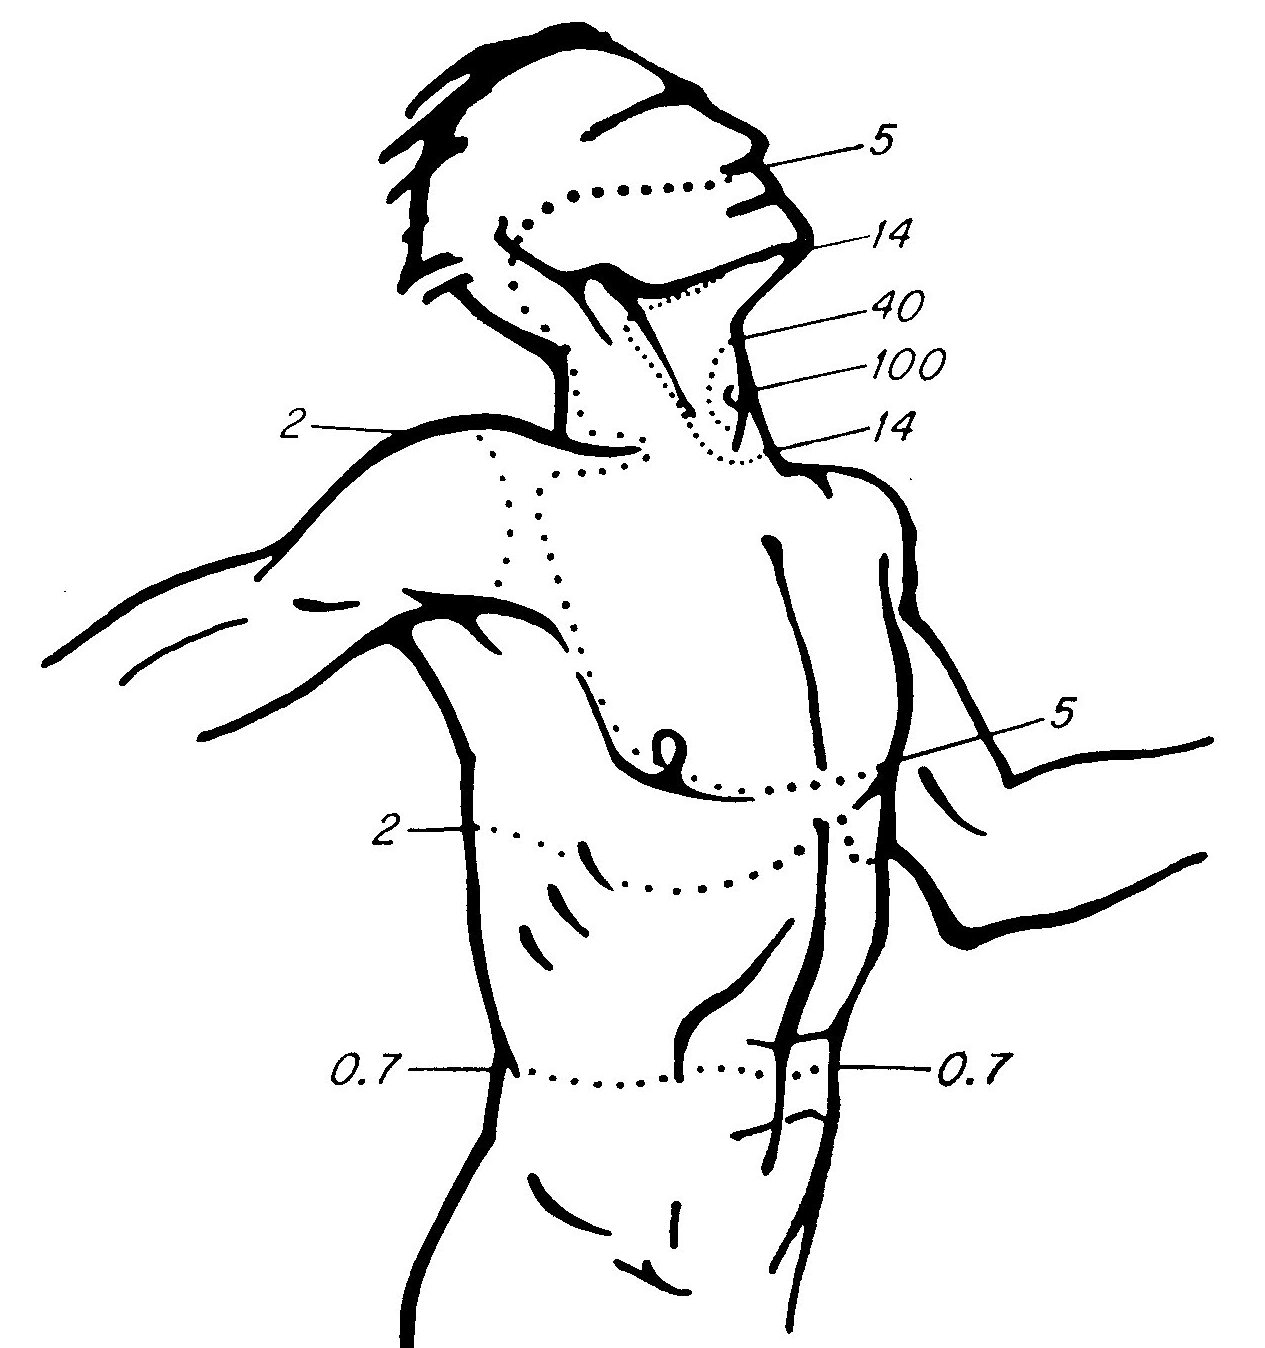
\includegraphics[width=0.5\textwidth]{figure/bekesy60-3b.png}
  \caption{Diagram of the propogation of speech waves throughout the body. Numbers correspond to percentage of the original amplitude of the speech remaining when reaching the marked location. Taken from \cite{bekesy:60}.}
  \label{fig:bekesyBodyTransfer}
%\end{figure}
\end{wrapfigure}

% Discussion about Body/Bone conduction (mechanical)

Bone conduction of acoustic vibrations through a human head has been well studied (cf. \cite{allen:60}, \cite{hakansson:94}, \cite{stenfelt:00}, \cite{reinfeldt:10}, etc); however most of these studies have involved attaching a mechanical vibration device to an animal head or a cadaver skull, or using a vibrating piston on a live human participant, allowing for precise manipulation of the input signal.  
%The acoustic vibrations resulting from the mechanical device positioned on the head propagate to and are recorded by a recording device on a different location on the head.  
Most of these studies, as well, are focused on audiometric bone conduction, i.e. the propogation of waves through the head and their effect specifically on the cochlea itself, which is not relevant to the present study.

%One study, \cite{hakansson}, used ``Live'' human subjects .  Titanium implants (pre-existing) for bone-conduction hearing aids anchored in the temporal bone behind the ear were used as the stimulation point for the mechanical vibrators.
Many of the early studies which were performed on cats do show that the sound generated by bone conduction propogating into the ear canal is dominated by low-frequency noise (\cite{tonndorf:72}).  Normally, the open ear acts as a high pass filter, dampening these lower frequencies passing into it via bone condution.  When occluded, this filter is non existant, and the lower frequencies are more noticeably present (discussed in depth further below). 

Other more recent studies on human subjects have agreed with these findings.  It has also been found that the acoustic response differs significantly depending on the location of the skull that is stimulated\footnote{Typically in these studies it is either the frontal bone or the mastoid process (\cite{bekesy:60}).}.
A few (cf. \cite{bekesy:48}, \cite{hansen:97b}, \cite{porschmann:00}, and \cite{reinfeldt:10}) have investigated body conduction when the source of vibration (i.e. sound) is a person's own voice, not an artificial mechanical vibrator.  These studies also record from the person's ear canal, and not another sensor on a different side of the skull.  

Using speech as a source is inherently messy, because 
\begin{enumerate*}[label={\alph*)}]
  \item  it is not as easily manipulated as a simple mechanical vibrator,
  \item  it has far more frequency components than a simple mechanical vibrator, and 
  \item  it takes multiple pathways to get to the ear: from the vocal chords, through tissue, and into the ear canal, and also from vibrations in the air all along the vocal tract\footnote{The speech sound is also filtered differently as it passes along the vocal tract}, through the solid medium of the head\footnote{Although, of course, the head is composed of different tissues with different densities and acoustic resonances}, and back into the medium of air inside the ear canal.
\end{enumerate*}
On top of this, the ear canal itself acts as a resonating chamber (\cite{rosen:91}), altering the signal beyond the distortion already caused by the passage through tissue and bone.  

% Discussion about EAC resonance Theory
% \begingroup
There has been much research on the resonating characteristics and amplitude response of the ear canal.  One such project was performed by \cite{stinson:89}, which studied fifteen human ear canals.  Their aim was to produce a model which can replicate the effect that the ear canal has on acoustics.
One challenge in producing such a model is the considerable variability in the shape of the canal - both between subjects as well as between the right and left ear canal of a single subject (\cite{stinson:89}).  These differences are apparent in curvature, length, volume, and cross-sectional diameter throughout the ear canal.  \cite{stinson:89} created silicon ear molds for each of the ear canals, which were used to generate three different computational models: one following the contours and dimensions of their ear molds exactly, another following the dimensions of the ear mold, but straightening contours and curvatures as if along a central axis, and the third as if the ear canal were a uniform tube with the same length and volume of the ear canal molds (and the previous models).  They noted that most significant differences between these models' spectral predictions of ear canal resonance occur above 6kHz (see fig. \ref{fig:eac_modelling}).  

Since much of the acoustic information for distinguishing speech sounds is located below 6kHz, several (cf. \cite{stinson:89}, \cite{hansen:97b} \cite{stenfelt:07}) who have made efforts to model the ear canal, have chosen to simply treat it as if it were a uniform tube.

Another challenge is to obtain the dimensions of the ear canal needed in order to treat it as a uniform tube in the first place. Immittance measurements are widely used in audiology, and involve emitting a chirp or tone into a pressurized ear canal.  The chirp then bounces back from the tympanic membrane (assumed to have infinite impedance in a pressurized canal) and can be recorded (\cite{ballachanda:97}, 415):``The sound pressure developed inside a rigid cavity from a known sound source is directly related to the volume of the cavity".  Therefore, the volume of the ear canal can be inferred for a subject using immittance testing without the need for invasive measurements (e.g. using a silicon mold).  Making an assumption about either an `average' diameter or an `average' length of the ear canal\footnote{The average length of the ear canal has been cited from 23mm (\cite{rosen:91}) up to approximately 29mm (\cite{stinson:89}) for a straight tube. The average diameter for the ear canal is approximately 7.1 mm (\cite{salvinelli:91}).}  would allow for the approximate calculation of the other dimension, given the measured volume. 
%These ear canal dimensions can then be plugged into any one of several models designed to approximate the ear canal dimensions.

\begin{wrapfigure}{L}{0.5\textwidth}
%\begin{figure}
\centering
  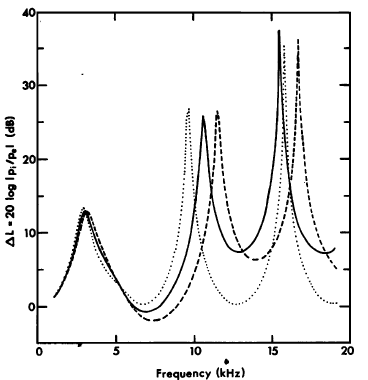
\includegraphics[width=0.5\textwidth]{figure/eac_mod_diffs.png}
  \caption{\cite{stinson:89} diagrams three different models of the ear canal resonance.  The bold line is based on their 3D canal molds from cadavers, the dashed line removes the curvature of the ear canal and acts as if the axis were straight, the dotted line assumes a constant diameter along a straight axis, with the same ear canal volume as the dashed and solid lines.}
  \label{fig:eac_modelling}
%\end{figure}
\end{wrapfigure}

% Discussion of the Occlusion Effect

Once inside the ear canal with known approximate dimensions, it can either be modeled as an open-closed tube (if the ear is not plugged) or as a closed-closed tube (if the ear is plugged). This difference changes the resonance and reverberant structure of the ear canal.
%BC+EC-OE
There have been many studies, a few in particular (c.f. \cite{bekesy:48}, \cite{porschmann:00}, \cite{reinfeldt:10}) which use real human speech and measure the human ear as an open-closed tube.

% \begingroup
\cite{porschmann:00}'s study is generally looking at the perception of one's own voice, but in order to accomplish this devotes effort to looking at the bone conduction pathway separately.  A general 900 Hz resonance (with subsequent harmonic resonances) was found in the collected bone-conduction speech, as well as a general broadband amplitude gain between 0.7 and 1.2 kHz.  This correlates with the 800-1200 Hz range for the first resonance that others  (cf. \cite{hakansson:94}) have observed in mechanical-stimulated bone conduction studies.  However, in this study only two phones were used (/s/ and /z/), and a masking threshold\footnote{The masking threshold technique involves playing a pure tone at different frequencies and amplitudes while the participant is phonating. The participant indicates when the tone becomes audible over their own speech, which allows the spectrum of the sound transmission of their speech to be mapped.} technique was used to determine the frequency spectrum of the transfer function of body conduction.  This is admittedly a rather subjective method of determining the spectrum.  

\cite{reinfeldt:10}, on the other hand, use microphones to record the actual sound pressure level (SPL) of both air and body conducted speech. Furthermore, \cite{reinfeldt:10} used a more expansive and diverse set of phones.  While a resonance was found in generally the same frequency region for /s/ (and other phones) as that found by \cite{porschmann:00} (0.7 - 1.2 kHz), they discovered some interesting differences, which can be seen in fig. \ref{BCrelAC}. Between each class that was used- voiceless sounds (/s/, /t/, /k/, and /tj/),  nasals (/m/ and /n/), and vowels (/i/, /e/, /a/, /o/) - a moderately similar frequency response is seen, yet there are some interesting distinctions to note (see fig. \ref{BCrelACall}.

In particular, as can be seen in fig. \ref{BCrelAC}, there is much inter-speaker variation within the body conduction of the same sound.  While it is difficult to track an individual speaker's relative spectral envelope within the figure, it appears that much of this difference, particular in the lower frequencies, originates from a difference in amplitude, and not necessarily from different resonance locations along the frequency axis.  It is important to note that both Figs. \ref{BCrelAC} and \ref{BCrelACall} both contain \textit{relative} spectral envelopes - i.e. the difference between the air conducted and body conducted components of speech, and do not contain an absolute frequency spectrum of body conducted speech. 

An interesting observation is that the /e/ vowel has a relatively flat response up to 500 Hz, and only dips down to -5 dB around 1kHz.  Contrast this with the phone /s/, which below 500 Hz has a fairly high (yet falling) response, and only dips below -5 dB near 4 kHz.  However, compared with /e/, the body conducted to air conducted ratio for /s/ has a significant downward slope after 2000 Hz.  This is likely due to the fact that there is relatively little energy produced by /s/ in the low frequencies, allowing for a high ratio, which drops as the general energy of the phone increases.  This could indicate that most of the energy produced by a non-sonorant does not pass through to the ear canal.

% \begin{wrapfigure}{L}{1.1\textwidth}
\begin{figure}
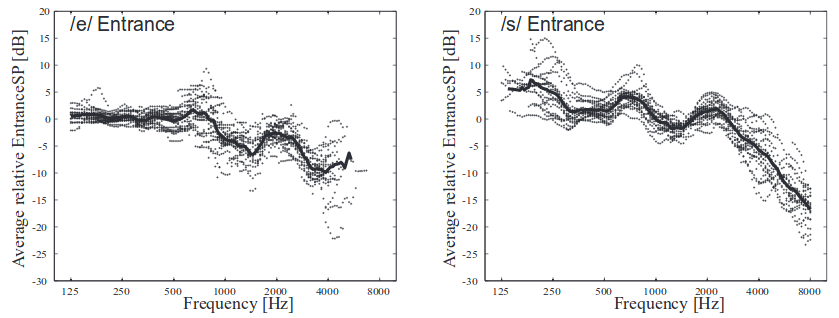
\includegraphics[width=1\textwidth]{figure/BCrelAC_e_s.png}
\caption{Body Conduction relative to Air Conduction for the phones /e/ and /s/.  A value of less than zero indicates the amplitude of body conducted speech is less than that of air conducted speech, and a value greater than zero indicates a higher amplitude of body conducted speech. The solid line indicates the mean, and the remaining data points are from individual speakers.  The signal was measured from the entrance of an open ear canal.  Taken from \cite{reinfeldt:10}.}
\label{BCrelAC}
\end{figure}
% \end{wrapfigure}

More specific dichotomies can be found between sounds within the same class. For example, the low vowel /a/ is pronounced with a more open mouth vs the relatively closed mouth of the high vowel /i/; consequently, the dB SPL relative to the air conducted counterpart was much higher for /i/ than it was for /a/. An assumption could be made from the data that the more open the mouth is, the more energy is transferred to the air conducted signal (cf. Fig. \ref{BCrelACall}).  This is supported by \cite{bekesy:60}, who also diagrammed the relative difference in amplitude in the ear canal between the air-conduction and body conduction of vowels (cf. Fig. \ref{bekesyPhoneDiff}), which also supports this hypothesis.  There was much inter-speaker variability, but it appears that the bone-conducted phones with the least relative reduction in amplitude are the higher vowels.  The more energy that is lost to air conduction during the production of low vowels, the less energy is transfered into the surrounding tissue.

\begin{wrapfigure}{L}{0.5\textwidth}
% \begin{figure}
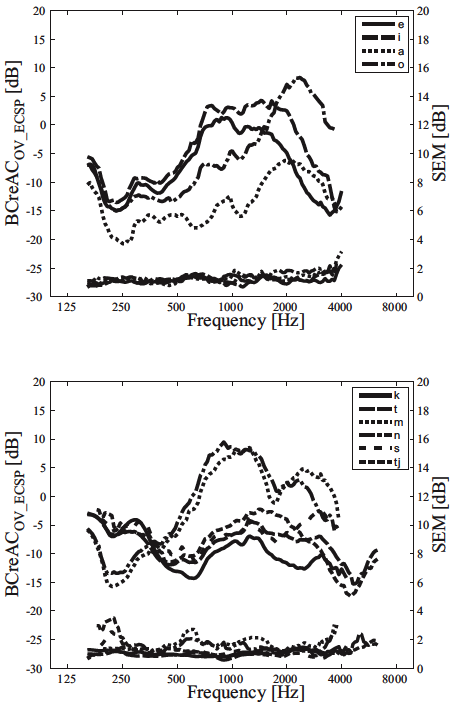
\includegraphics[width=0.5\textwidth]{figure/BC_rel_AC_all.png}
\caption{The mean relative amplitudes (left ordinate) of body conduction relative to air conduction for vowels (top plot) and other sounds (bottom plot).  The set of lines along the bottom of each plot represent the standard error from the mean (SEM), measure on the right ordinate.  Taken from \cite{reinfeldt:10}.}
\label{BCrelACall}
% \end{figure}
\end{wrapfigure}

% \endgroup

% \begingroup
Additionally, \cite{reinfeldt:10} found that the mid back vowel /o/ has a distinctive spectrum in relation to the other vowels, in which there is an amplitude peak near 2 kHz, rather than 1 kHz.  Since the functions of other high back sonorants /u/ and /\textipa{N}/ are not given, we cannot be certain if this is a phone-specific difference, or if it can be generalized to higher ``back" articulations in which the articulatory constriction restricting the acoustic engergy is further back in the vocal tract.\footnote{\cite{bekesy:60} does not break down relative amplitude by frequency}  It is also important to re-emphasize that these transforms are given as body conducted amplitude \textit{relative to} air conducted amplitude for the given phone, and do not reflect the absolute air- and body-conducted amplitude of phones compared with one another.  For example, /a/ is a relatively loud air conducted sound due to its open articulation, and this loud air conducted component may cause its \textit{relative} body conducted component to appear quieter than the other vowels, when in reality it is possible that the body conducted component of both vowels have the same absolute amplitude.  Neither \cite{bekesy:60} nor \cite{reinfeldt:10} give information about body conducted components in relation to one another.


\begin{wrapfigure}{R}{0.5\textwidth}
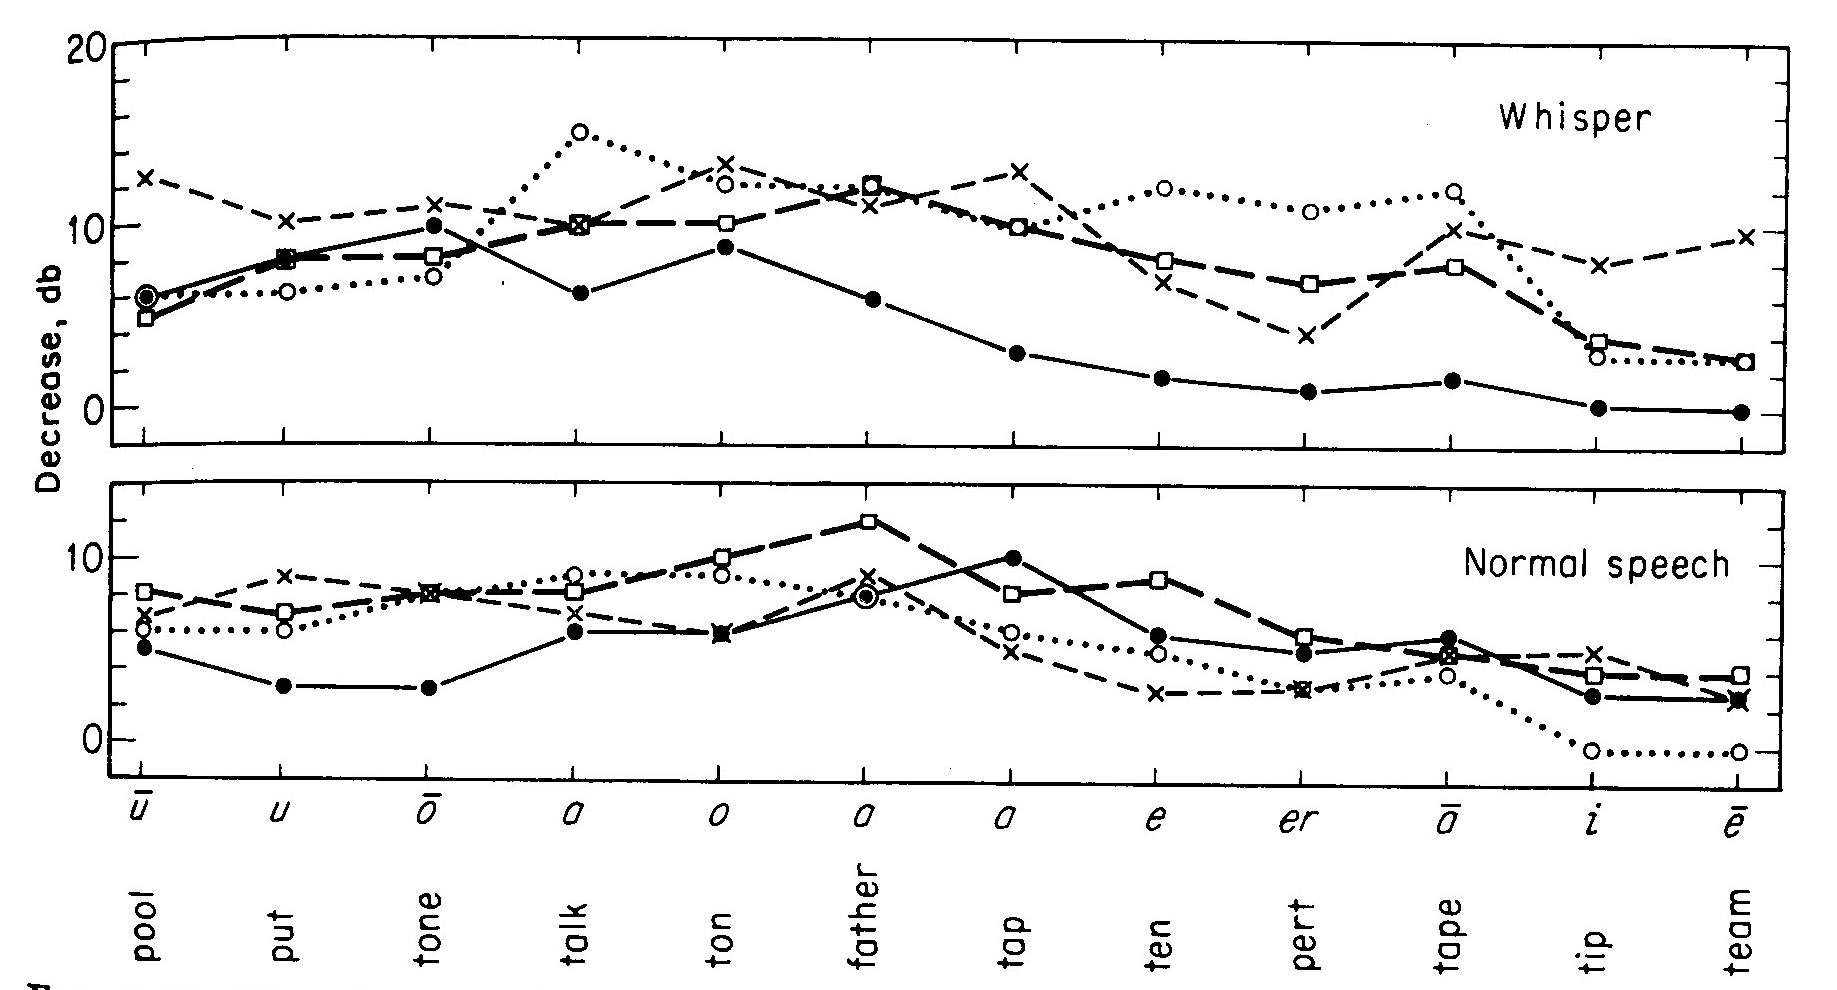
\includegraphics[width=0.5\textwidth]{figure/bekesy60-3.png}
\caption{Demonstrated the different effect on amplitude that closing the ear canal has on the different vowels of English.  Taken from \cite{bekesy:60}.}
\label{bekesyPhoneDiff}
\end{wrapfigure}

%BC+EC+OE

Modelling the ear as a closed-closed tube, however, results in a slightly different frequency response.  This phenomenon, first noted by \cite{wheatstone:79}, is termed the occlusion effect (OE).  The occlusion effect\footnote{The occlusion effect is the change in sound pressure level (SPL) resulting from body conducted vibrations emanating into, and reverberating within, a \textit{closed} ear canal.} (OE) offers an amplitude gain to certain frequencies and dampens others.  This has been studied widely and extensively (cf. \cite{wheatstone:79}, \cite{kelly:37}, \cite{littler:52}, \cite{goldstein:65}, among many others).  Generally, the occlusion effect (OE) results in a great increase in the amplitude of frequencies below 1-2kHz, acting as a low-frequency gain and that the amplitude of higher frequencies is dampened (as previously mentioned in the observation in studies of cats (\cite{tonndorf:72}).

%\cite{hansen:97b} and \cite{stenfelt:07} are primarily interested in modelling an occluded EAC, and this study requires the model to be a closed-closed tube - that of an \textit{occluded} ear. The models proposed by \cite{hansen:97b} and \cite{stenfelt:07} take many parameters, yet most can be considered to be either \textbf{too difficult to calculate frequently (- what does this mean? give an example)}, or relatively constant (e.g. the impedance of the middle ear, the speed of sound, etc.).  Both models, however, take the parameters for the length of the EAC, the average cross sectional area or diameter, and the volume of the EAC, which, are highly variable.

 
As with bone conduction in general, most of the research of the occlusion effect (OE) has been conducted using controlled mechanical vibrations.  \cite{bekesy:60} reports that when the ear canal is closed, there is an increase in amplitude up to 2kHz, which afterwards vanishes quite suddenly (cf. fig. \ref{fig:bekesyOEresponse}).

\begin{wrapfigure}{R}{0.5\textwidth}
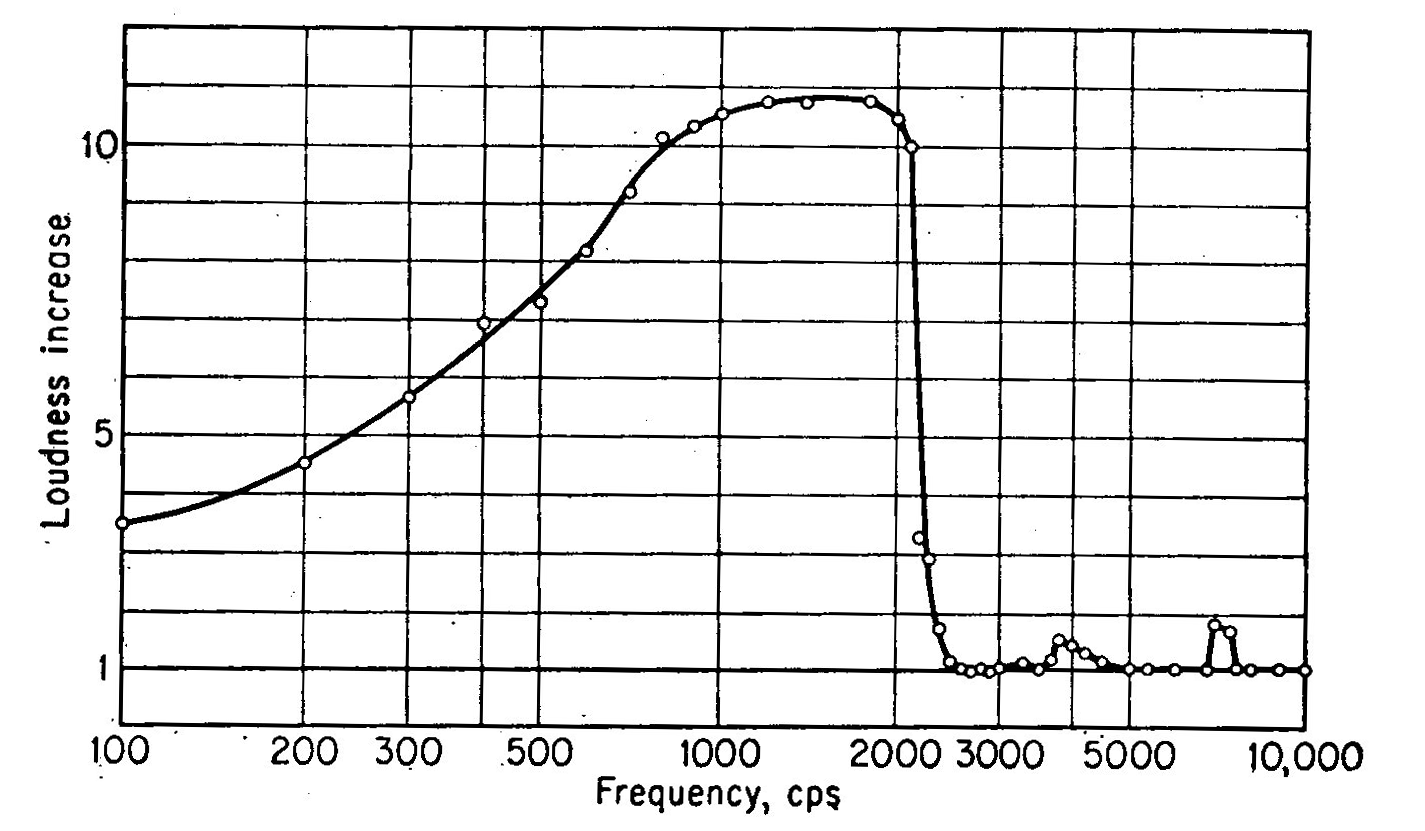
\includegraphics[width=0.5\textwidth]{figure/bekesy60-1.png}
\caption{The frequency response inside the ear canal when taking a mechanical vibrator to a participant's forehead.  Taken from \cite{bekesy:60}.}
\label{fig:bekesyOEresponse}
\end{wrapfigure}

However, there is a variance in the OE - if using a mechanical vibrator - depending on the location of stimulation.  This difference is most present in the lower frequencies (\cite{dean:00}), where the relative amplitude increase (of body-conducted sound versus air-conducted sound) appears to be the greatest, but tends to wash out when slightly higher frequencies are reached\footnote{\cite{dean:00} found that the greatest relative amplitude increase occurs near 250 Hz, but the gain disappears when 1000 Hz is reached.}.  There are also differences based on the location of \textit{occlusion} within the ear canal, i.e. how deep a plug is placed in the ear canal. \cite{dean:00}'s results indicate this difference does not disappear as frequency increases; the relative amplitude increase is greatest with supra-aural earmuffs at lower frequencies, and lowest with deep inserted earplugs\footnote{\cite{dean:00} does not mention the explicit the depth for each condition, but from the article's description of the insersion procedure, it appears to be \~5mm.}. However, at 1 kHz, the shallow-inserted earplug has a greater relative amplitude gain than the supra-aural earmuff.

\cite{stenfelt:07} developed a model of an occluded ear using measurements generated from stimulating the skull separately at both the frontal bone and the mastoid process.  Each site yielded a slightly different frequency response for the occlusion effect.  Stimulation at the mastoid generally resulted in a greater increase in very low frequencies below 1 kHz.  They also noted that the OE was greatest when using an ear plug near the opening of the ear canal, as opposed to supra-aural `ear muffs' or a deep-insersion ear plug, though an OE was noticeable in each condition; this is in direct contrast with \cite{dean:00}.  \cite{dean:00} do not mention the size of earmuff used, but \cite{stenfelt:07} report the use of a large and small earmuff, with the latter providing a greater OE than the former, though both still below that of the shallow-insertion earplugs.
With shallow insersion, their model estimates a gain in amplitude of frequencies below 2 kHz, and dampening of those above; all insersion depths, according to their model, will at minimum, slightly dampen frequencies above 2 kHz.  As the plug is inserted deeper, the damping occurs on lower and lower frequencies. These results contrast slightly with \cite{bekesy:60}'s in fig. \ref{fig:bekesyOEresponse} in that they predict higher, very low frequencies, as opposed with \cite{bekesy:60}'s resonance around 1-2kHz.


In contrast to the mechanical source studies above, \cite{hansen:97b} tested the OE using one's own voice as the input source.  \cite{hansen:97b} presents a graph comparing three spectra calculated from continuous speech from three separate publications\footnote{From \cite{wimmer:86}, \cite{thorup:96}, and \cite{may:92}} (Fig. \ref{fig:hansenAverageOEa}).  The study conducted its own tests (seen in Fig. \ref{fig:hansenAverageOEb}), which, by and large, agree with the previous studies.  These represent the `average' effect of occlusion on speech, and appears to resemble other (mechanical-source) estimations.  \cite{hansen:97b} developed a model of the OE which largely agrees with these measurements.

The studies looking at human speech result in similar spectral resonances as those dealing with simple mechanical vibrations, except real-speech studies are able to capture the different OE for different kinds of complex sounds in a real speech environment, such as vowels.  

% \begingroup

% \begin{wrapfigure}{R}{1\textwidth}
\begin{wrapfigure}{R}{0.5\textwidth}
\begin{subfigure}{0.5\textwidth}
  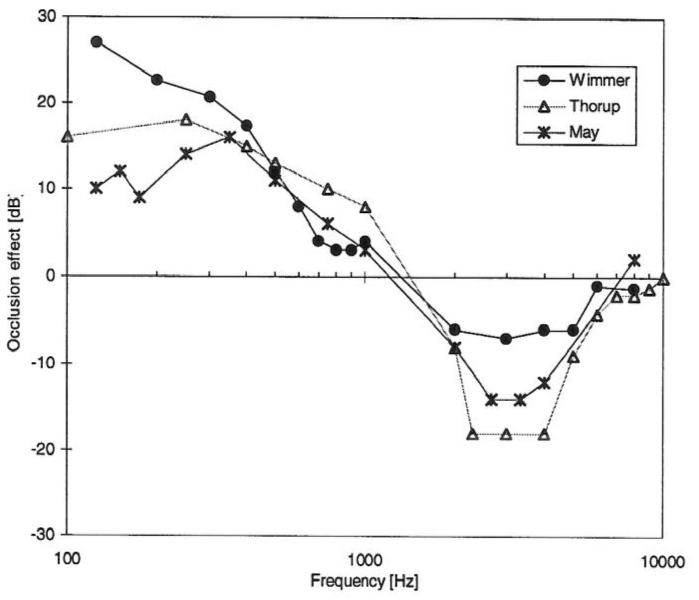
\includegraphics[width=1\textwidth]{figure/hansenAverageOE.png}
  \caption{ }
  \label{fig:hansenAverageOEa}
\end{subfigure}%
\hfill
\begin{subfigure}{0.5\textwidth}
  \begin{subfigure}{1\textwidth}
    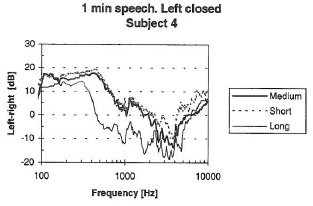
\includegraphics[width=1\textwidth]{figure/Hansen_OE-plot_a.png}
  \end{subfigure}
  \begin{subfigure}{1\textwidth}
    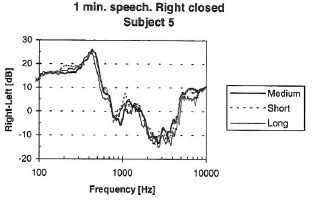
\includegraphics[width=1\textwidth]{figure/Hansen_OE-plot_b.png}
  \end{subfigure}
  \caption{ }
  \label{fig:hansenAverageOEb}
\end{subfigure}
\caption{In (a), three separate measured OE spectra. In (b), a comparison of the measured occlusion effect (OE) between two subjects and different sized ear molds that extend into the ear canal at different lengths. Taken from \cite{hansen:97b}.}
\label{fig:hansenAverageOE}
\end{wrapfigure}
% \end{wrapfigure}

%% Allaying concerns of the effect of jaw movement on the occlusion effect.
While \cite{hansen:97b} found phone-specific differences in the occlusion effect (OE), it is ambiguous as to whether the differences are solely due to the differences in the transforms of phones as a result of body conduction (as seen in \cite{reinfeldt:10}), or if there are sound-specific differences introduced within the ear canal or by the occlusion effect itself.  Some have posited that variablility could critically stem from the placement of the jaw bone during speech next to the external auditory meatus, and as that changes as the jaw moves up and down\footnote{Thereby changing the impedance characteristics of the vibration, (\cite{bekesy:60})} for `higher' or `lower' phones (e.g. /i/ vs /a/).  \cite{allen:60} studied the OE on participants with a unilateral resection of the mandible (one side of the jaw has been removed), and found essentially no distinction between the OE in either ear (i.e. with a mandibular joint adjacent to the cartilage of the ear canal or without).

Yet, \cite{hansen:97b}) found that a change in shape of the ear canal due to different jaw positions can create an acoustic ``leak" between the ear canal wall and the occlusion device; the occlusion effect, obviously, behaving differently for different levels of occlusion. 
\cite{hansen:97b} diagrams cross sections of the ear canal with the jaw at different positions; between a closed jaw and 5mm of opening, there is relatively little difference between the shapes of the ear canal.  Since \cite{borghese:97} found that the jaw moves relatively little vertical distance during actual speech (max opening approx. 6 mm), it can be assumed that the ear canal changes shape negligibly during normal speech with a snug-fitting occlusion device. 

In summary, it is important to emphasize the key difference between measurements from an occluded ear canal and those from an open ear canal, which can largely be seen between figs. \ref{BCrelACall} and \ref{fig:hansenAverageOEa}.  There is a massive increase in the amplitude of the lower frequencies, which is not present from an open-closed ear canal, and a sizeable drop in amplitude after 2kHz, which similarly does not seem to manifest itself when the ear canal is not occluded.


%CONCLUSION

The aforementioned studies on body conduction and the occlusion effect, as would be expected, have indicated a fair deal of inter-person and inter-phoneme variability, and have shown the complexity involved in estimating the effect of body conduction and ear canal reverberance on speech entering the ear canal.  However, the transfer function from the vocal tract to the ear canal does have some standard characteristics, namely, the body and (occluded) ear canal act as a low-pass filter on speech, removing many of the higher frequencies which are within range of containing critical components for speech intelligibility.

%CONCLUSION to expt 1 lit review

%There is a possibility that the ear signal might be so low-pass filtered as to dampen the upper frequencies beyond retrieval and to the point that accurate recognition is unlikely.  In this case, there are still several possibilities, one of which will be outlined below.  

%While critical speech information may be lost, there is still critical speech information that will be present in the signal, namely the pitch.  The ear signal could be used to ``clean" a simultaneously recorded signal obtained from the mouth (which includes any ambient noise).  Since the occlusion effect acts as a gain in the low frequencies, the harmonic information of the voice signal can be reliably obtained from the ear signal.  Using this harmonic information, a comb filter (cf. \cite{nehorai:86}) could be developed and applied to the noisy mouth signal (cf. \cite{king:08}, \cite{cai:09}, \cite{jin:10}).  The comb filter acts as a series of narrow bandpass filters at equal (harmonic) intervals; when applied to speech, this can filter out the noise located in-between the harmonics.  

%There are a number of drawbacks with this method, however.  One is that this method primarily is used to recover voiced (harmonic) sounds, and fricatives or other voiceless sounds may not be able to be `cleaned'.  Another is that while speech is generally harmonic-like, it is not a perfectly harmonic signal, and there is a possibility that some of the higher harmonics might be accidentally filtered out.  This is particularly concerning as the higher frequencies are what is missing from the ear-recorded signal in the first place.


The methods described in this section, namely the models and transfer functions used by \cite{hansen:97b}, \cite{stenfelt:07}, and \cite{reinfeldt:10}, predict a general rise in amplitude of lower frequencies (below 2 kHz), and a drop in frequencies above that range (with a few exceptions).  This distortion is hypothesized to be predictable, unlike ambient noise from the environment, which is generally highly variable in both amplitude and form.  Due to this, the technique of substituting unpredictable noise with the ``predictable noise" of body conduction and the occlusion effect allows for greater confidence that a usable signal will be recovered.  The ``recovered" signal after undergoing minor transformations is hypothesized to perform better than a noisy signal collected from the mouth in both ASR and human speech perception tasks.  Section \ref{expt1} below describes the specific methods used to collect speech data from the mouth and the ear canal and recover an intelligible signal from the latter using the principles outlined in this section.


\section{Experiment 1: Creating a dataset of ear-recorded speech\label{expt1}}

Due to the numerous constraints and requirement for the speech recordings required for this task it was necessary to create an original dataset for this study. 

\subsection{Design}
   
The goal of this experiment was to create a dataset of recordings, both from the mouth, in noisy conditions, and from inside the ear in the same conditions.  These recordings needed to demonstrate that (a) by recording speech from the ear, external noise was completely or largely eliminated, while simultaneously recorded speech from the mouth had a noisy background, (b) that the speech from the ear was more intelligible and recognizeable by humans than noisy speech, and (c) that the speech from the ear was more intelligible and recognizeable by an ASR system than noisy speech. 

In alignment with the CHiME challenge\footnote{The CHiME challenge tasks researchers to improve upon or surpass the performance of a baseline automatic speech recognizer used on noisy speech data.} guidelines, this study uses different types of background noise at different noise levels.  The noises used include the four sounds (bus, cafe, pedestrian area, \& street) from the CHiME\cite{chime:16} challenge, plus a `factory' noise track.  A short portion of the audio with relatively level amplitude was extracted from each sound file to be played in the background.\footnote{\textbf{The exact portions of these sounds which were used are available online, along with the rest of the data at URL.COM}}

Three noise levels were used.  Since conversational speech is generally around 70 dB, the noise levels chosen were 60 dB, 70 dB, and 80 dB\footnote{These were the `averaged' dB levels over the course of the sound file}.  This would result in approximate SNR conditions of +10 (60 dB), 0 (70 dB), and -10 (80 dB).  80 dB was also chosen as a max loudness in order to leave a wide margin between it and any (albeit remote) possibility of hearing damage. A `clean' condition was also utilized (no noise).  Thus far this creates 16 different conditions (5 noise types * 3 noise levels + 1 `clean' condition).  

\subsection{Stimuli}
Thirty sentences were chosen from 3 Harvard Sentence lists\footnote{The `Harvard Sentences' is comprised of 72 lists, each 10 sentences long, where each list of 10 sentences is phonetically balanced, where the proportion of each phone in the list corresponds with it's occurrence in the English language.\cite{harvardsentenceURL}}.  Lists 14, 28, and 57 were used, and chosen semi randomly, eliminating lists with potentially unfamiliar or rare words.  Each sentence occurs in all 16 conditions, resulting in 480 total stimuli.

  
\subsection{Equipment}

The experiment took place in a XXXX soundbooth.  To create the artificially noisy environment a Yamaha MS101 III loudspeaker was hooked to an HP ProBook 6470b laptop.  A sound pressure level meter (SPL meter; Larson Davis Model 831) with a PCB Piezotronics Model 377B20 condenser microphone (omnidirectional) was placed 1 meter from the loudspeaker and measured the sound pressure to verify each of the three noise levels for each of the 5 noise types. A Grason-Stadler GSI Typstar Middle Ear Analyzer was used to measure the ear canal volume and test for plug leaks.  Two Countryman B2D directional lavalier microphones with fixed XLR connections were used to record the mouth speech and the ear speech.  These were hooked up to a PreSonus Digital Audio Firebox preamplifier, which was connected via TRS cables to a Zoom H6 Handy Recorder. A pair of 3M Professional Peltor Earmuffs with an NRR of -30 dB SPL were worn by the participant during the experiment.


\subsection{Participants}
Twenty participants were used in this study, ten female and ten male, all native speakers of English with normal hearing.

\subsection{Procedure}

The participant is initially asked a few preliminary demographic questions\footnote{e.g. 2nd language (if any), etc. For a list of all information gathered, see Appendix A\ref{appendixB}.}. They are seated in front of the Middle Ear Analyzer.  An otoscope is used to ensure the ear is mostly free of cerumen, to avoid blocking the microphone off from the rest of the canal or generally impacting the canal with cerumen.  The chosen ear is fitted with an appropriate sized rubber clinical single-use ear tip, into which the Middle Ear Analyser hose is already plugged.  An immittance test is performed, which involved playing a tone, and slightly and briefly pressurizing the ear.  The Middle Ear Analyser checks that the ear plug solidly seals off the ear canal in order to be able to build up pressure, and alerts the researcher to a leak if the plug is not securely in place.  This test results in an estimate of the volume in milliliters (mL) of the ear canal and of the middle ear, with precision to a tenth of a mL; additionally, a graph of middle ear function is given, which is checked for normalcy (cf. Appendix B\ref{appendixB}).  Several other measures are given which are not used in this study.

The distance from the end of the ear plug to where it is enclosed by the ear canal is measured to determine how far the plug was placed in the ear canal (cf. Fig. \ref{earplugInserted0.png} for diagram).  Since the length of the plug is known, this was done by placing a measuring rod against the cavity of the concha to measure how far the plug was sticking out of the ear. The decision to treat the cavity of the concha as the ``end" of the ear canal is taken from \cite{stenfelt:07}, who made molds of ear canals, and treated the rapid increase in volume (where the cavity of the concha begins) as the end to the ear canal.  This measure allows for the calculation of the depth of insersion of the earplug.

The Middle Ear Analyser hose is then taken out of the ear plug - which is carefully left in place to ensure a continuous seal.  The participant then moves to a seat located in front of a computer monitor.  The loudspeaker is on another table to the right of the participant, perpendicular to the direction the participant is facing (cf. Fig \ref{overallSetUp1.png} for set-up diagram).  The participant is then instructed as to the proceedings of the rest of the experiment. One of the two microphones is taken, the wind-break foam removed, and is snugly inserted into the ear plug.  A mark on the microphone cable was used to ensure the end of the microphone was fully inserted to the end of the earplug.  Occasionally, the microphone was inserted deeper than, or just shy of, the end of the ear plug; the variance is within +/-1mm depth (cf. Appendix B\ref{appendixB}).  The earmuffs are placed over both ears.  Occasionally, a participant had glasses, or thick hair, which may have slightly compromised the seal.  A note was taken of this. 

A wooden rod was attached to the ear muffs, which extends forward, beside the participant's face.  The second microphone was attached to this wooden rod via the lavalier clip at the level of the participant's mouth.  The microphone was directed toward their mouth (cf. Fig \ref{microphoneDetailSetup2.png}).  The placement of the microphone on the wooden rod was adjusted to be exactly 10cm away from the participant's infra-nasal depression.  At this point, the participant was asked to adjust the placement of their chair so that the microphone on the wooden rod was approximately 1 meter from the loudspeaker. Due to the length of the experiment (~45min), no effort was made to discourage minor shifting in body position.  

Both microphones were connected directly to the preamplifier through a fixed (non-changeable) XLR connection.  Both channels were set to the same gain on the preamplifier.  Two TRS cables took each microphone signal from the preamplifier to the recorder.  Both channels were adjusted to appropriate (different) gain levels on the recorder itself to achieve a similar loudness for both signals and prevent clipping.  These adjustments were made once the participant was situated, but before beginning the recording.

Once recording, an in-house computer program was used to display the stimuli sentences on a second monitor and play the background noises.  For each sentence, the participant saw the clean-condition (no noise) first.  The researcher was in the soundbooth with the participant listening through a pair of headphones connected to the preamplifier.  The participant was asked to repeat the sentence twice to get a rhythm for it, at a normal, conversational loudness, with a normal, declarative intonation.  The researcher asked the participant to repeat the sentence again in this condition if the rhythm or intonation of the two sentences did not match, or if the participant stumbled over a word.  Each of the following 15 iterations of the sentence (one for each noise-type/noise-level combination) the participant was instructed to speak only once.  If the rhythm of the sentence varied noticeably, or if a sentence was stumbled over, the researcher again asked the participant to repeat the sentence for that condition.  The sentences were not randomized, i.e. all 16 iterations of a sentence occurred consecutively\footnote{This was done to enable to researcher to ensure a similar intonation and rhythm for each iteration of a given sentence.}. Within each sentence group (after the first, `clean' condition, which always occurred first), all the noise conditions were randomized. Each stimulus is advanced by the researcher.

To help the participant notice when a sentence had been advanced\footnote{Wearing the ear muffs, they were often not aware when the noise condition changed.}, the number of the sentence condition was displayed underneath the stimulus (i.e. 1-16).  This had the unindended consequence of occasionally producing a mild list-intonation. 

After the recording was finished, the participant was asked to complete a short, 4 question survey\footnote{cf. Appendix C\ref{appendixC} for exact (non-coded) survey answers} of their experiences during the experiment.  They were instructed to give as basic or as detailed answers as they wished, but to answer truthfully.  Extra credit in a Linguistics or other participating course was offered in exchange for participation in the experiment.

\section{Experiment 1 Analysis}

Each individual sentence was isolated in each recording with a Praat textgrid and extracted; this resulted in a sound file for each sentence, for each participant, for both the mouth-recorded and ear-recorded speech.  Figures \ref{spctgrmNarrowMouth_35}, \ref{spctgrmWideMouth_35}, \ref{spctgrmNarrowEar_35}, and \ref{spctgrmWideEar_35} show the narrow and wide band spectrograms for ear- and mouth-recorded speech from participant 35, a female, for a ``clean'' example of the sentence ``A cramp is no small danger on a swim''.  These two examples are fairly representative of the speech collected from each location.

\begin{figure}
\centering
\begin{subfigure}{.5\textwidth}
  \centering
  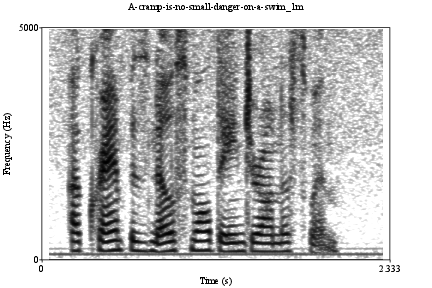
\includegraphics[width=1\linewidth]{figure/spctgrmNarrowMouth_35.pdf}
  \caption{spctgrm Narrow Mouth 35}
  \label{spctgrmNarrowMouth_35}
\end{subfigure}%
\hfill
\begin{subfigure}{.5\textwidth}
  \centering
  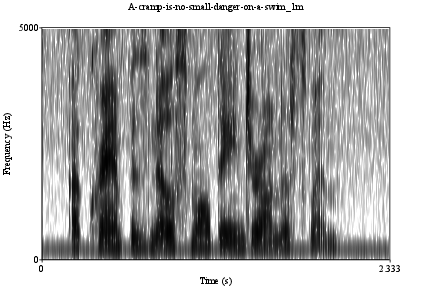
\includegraphics[width=1\linewidth]{figure/spctgrmWideMouth_35.pdf}
  \caption{spctgrm Wide Mouth 35}
  \label{spctgrmWideMouth_35}
\end{subfigure}
\caption{FIGURE CAPTION}
\label{fig:spect_mouth}
\end{figure}


\begin{figure}
\centering
\begin{subfigure}{0.5\textwidth}
  \centering
  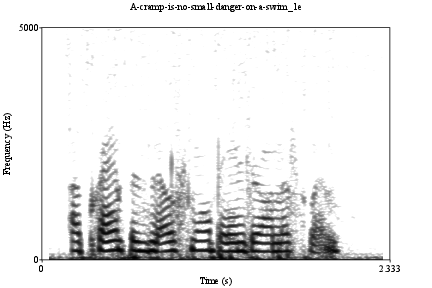
\includegraphics[width=1\linewidth]{figure/spctgrmNarrowEar_35.pdf}
  \caption{spctgrm Narrow Ear 35}
  \label{spctgrmNarrowEar_35}
\end{subfigure}%
\hfill
\begin{subfigure}{0.5\textwidth}
  \centering
  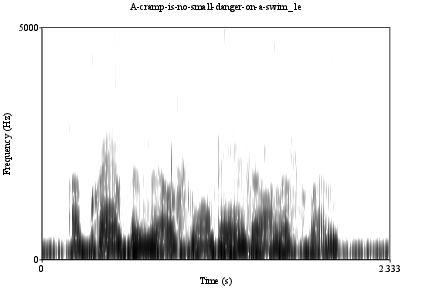
\includegraphics[width=1\linewidth]{figure/spctgrmWideEar_35.pdf}
  \caption{spctgrm Wide Ear 35}
  \label{spctgrmWideEar_35}
\end{subfigure}
\caption{FIGURE CAPTION}
\label{fig:spect_ear}
\end{figure}


As can be seen, the speech collected at the ear is heavily low-pass filtered, and the mouth speech by itself has much more speech information.
However, there are still clear harmonics in the existing range in the ear-recorded speech, and most of the lower two formants can also be seen.

When noise is present, it can be seen in Figs. \ref{spctgrmNarrowMouthNoise_35} and \ref{spctgrmNarrowEarNoise_35} that the noise does not affect the ear recorded signal nearly as much.  There appears to be some of the louder noise (seen in the mouth-recorded speech in fig. \ref{spctgrmNarrowMouthNoise_35}) present in the upper frequencies of the ear recorded speech, but it is significantly dampened and the signal has an overall higher speech to noise ratio (SNR).

It should also be noted that the SNR in fig. \ref{spctgrmNarrowMouthNoise_35} is much lower than originally intended.  For this particular example, the speech was recorded with an 80dB noise background, with the intent of obtaining a -10dB SNR.  Instead, the SNR is 6 dB\footnote{The SNR was calculated by using background noises recorded in isolation in the soundbooth.  These were recorded at 60, 70, and 80 dB in the same soundbooth, with the same conditions and set up as a normal recording.  The speech sound file was passed through a Hilbert Envelope, and a threshold was applied in order to extract just the speech data.  The RMS values of both the speech and noise vectors were calculated, averaged, and then used in the SNR calculation.  For explicit code, see Appendix E\ref{appendixE}}.  This is attributed to a) the participant speaking louder than anticipated, resulting in a higher speech theshold, and b) the directionality of the microphone used eliminated much more background noise than anticipated.

\begin{figure}
\centering
\begin{subfigure}{0.5\textwidth}
  \centering
  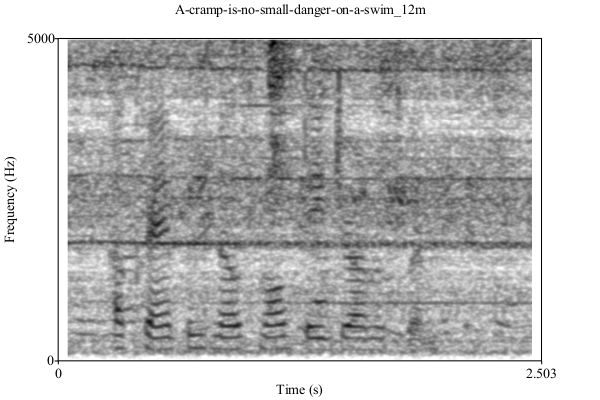
\includegraphics[width=1\linewidth]{figure/spctgrmNarrowMthNoise_35.pdf}
  \caption{spctgrm Narrow Mth Noise 35}
  \label{spctgrmNarrowMouthNoise_35}
\end{subfigure}%
\hfill
\begin{subfigure}{0.5\textwidth}
  \centering
  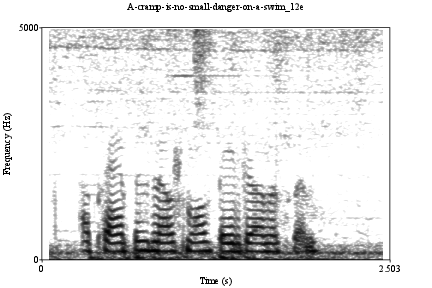
\includegraphics[width=1\linewidth]{figure/spctgrmNarrowEarNoise_35.pdf}
  \caption{spctgrm Narrow Ear Noise 35}
  \label{spctgrmNarrowEarNoise_35}
\end{subfigure}
\caption{FIGURE CAPTION}
\label{fig:noise_mth_ear}
\end{figure}

In an attempt to see if there are recoverable frequencies in the higher ranges, the ear speech was preemphasized, seen in fig \ref{spctgrmNarrowEarNoisePremp_35}, which has been placed next to its non-preemphasized counterpart for comparison.  It appears that while those fainter harmonics in the midrange frequencies have become more pronounced, there is no new speech information in the upper frequencies which has made it past the noise threshold.  To be certain, the spectrogram range of the non-premphasized ear signal was increased from 5kHz to 20kHz (see fig. \ref{spctgrmEarNarrowNoise_35_20kHz}). There is certainly acoustic energy that makes it to the higher frequencies, but there does not appear to be harmonics, nor does any of the visible acoustic energy appear to correlate with the speech seen in the lower frequencies.

\begin{wrapfigure}{L}{0.5\textwidth}
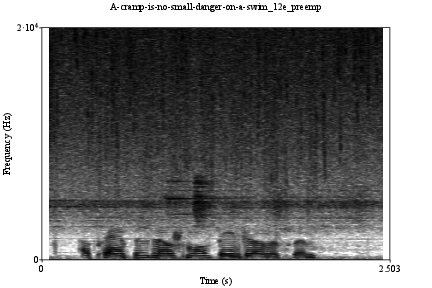
\includegraphics[width=0.5\textwidth]{figure/spctgrmNarrowEarNoisePremp.pdf}
\caption{spctgrm Narrow Ear Noise P 35}
\label{spctgrmNarrowEarNoisePremp_35}
\end{wrapfigure}

This ear-recorded signal was then low-pass filtered at 2500 Hz with a 500 Hz smoothing slope. To further emphasize the higher frequencies (and to smooth over the 'muffled' attribute a bit), the sound was preemphasized a second time (after filtering).  This can be seen in Figure \ref{spctgrmNarrowEarNoisePrempFiltPremp_35}, next to the noisy mouth speech for comparison \ref{spctgrmNarrowMouthNoise_35_compare}.

\begin{figure}
\centering
\begin{subfigure}{0.5\textwidth}
  \centering
  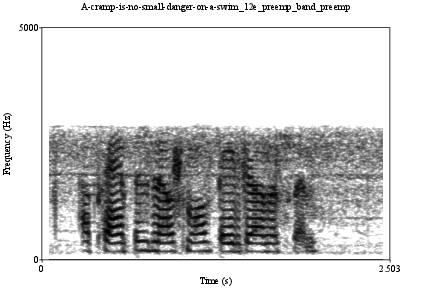
\includegraphics[width=1\linewidth]{figure/spctgrmNarrowEarNoisePrempFiltPremp.pdf}
  \caption{spctgrm Narrow Ear Noise PFP 35}
  \label{spctgrmNarrowEarNoisePrempFiltPremp_35}
\end{subfigure}%
\hfill
\begin{subfigure}{0.5\textwidth}
  \centering
  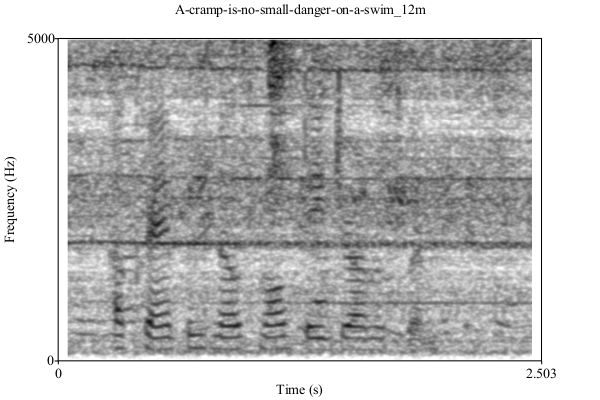
\includegraphics[width=1\linewidth]{figure/spctgrmNarrowMthNoise_35.pdf}
  \caption{spctgrm Narrow Mth Noise 35}
  \label{spctgrmNarrowMouthNoise_35_compare}
\end{subfigure}
\caption{FIGURE CAPTION}
\label{fig:ear_pfp}
\end{figure}

\section{Summary and Discussion}
Here is my summary and discussion. \textbf{Mention the limitations - namely the directionality of the microphone affecting the lack of noisyness in the data}







\bibliographystyle{apa}
\bibliography{DissRefs.bib}
\end{document}

\documentclass[dissertation,copyright]{uathesis}
\usepackage[]{graphicx}\usepackage[]{color}
%% maxwidth is the original width if it is less than linewidth
%% otherwise use linewidth (to make sure the graphics do not exceed the margin)
\makeatletter
\def\maxwidth{ %
  \ifdim\Gin@nat@width>\linewidth
    \linewidth
  \else
    \Gin@nat@width
  \fi
}
\makeatother

\definecolor{fgcolor}{rgb}{0.345, 0.345, 0.345}
\newcommand{\hlnum}[1]{\textcolor[rgb]{0.686,0.059,0.569}{#1}}%
\newcommand{\hlstr}[1]{\textcolor[rgb]{0.192,0.494,0.8}{#1}}%
\newcommand{\hlcom}[1]{\textcolor[rgb]{0.678,0.584,0.686}{\textit{#1}}}%
\newcommand{\hlopt}[1]{\textcolor[rgb]{0,0,0}{#1}}%
\newcommand{\hlstd}[1]{\textcolor[rgb]{0.345,0.345,0.345}{#1}}%
\newcommand{\hlkwa}[1]{\textcolor[rgb]{0.161,0.373,0.58}{\textbf{#1}}}%
\newcommand{\hlkwb}[1]{\textcolor[rgb]{0.69,0.353,0.396}{#1}}%
\newcommand{\hlkwc}[1]{\textcolor[rgb]{0.333,0.667,0.333}{#1}}%
\newcommand{\hlkwd}[1]{\textcolor[rgb]{0.737,0.353,0.396}{\textbf{#1}}}%
\let\hlipl\hlkwb

\usepackage{framed}
\makeatletter
\newenvironment{kframe}{%
 \def\at@end@of@kframe{}%
 \ifinner\ifhmode%
  \def\at@end@of@kframe{\end{minipage}}%
  \begin{minipage}{\columnwidth}%
 \fi\fi%
 \def\FrameCommand##1{\hskip\@totalleftmargin \hskip-\fboxsep
 \colorbox{shadecolor}{##1}\hskip-\fboxsep
     % There is no \\@totalrightmargin, so:
     \hskip-\linewidth \hskip-\@totalleftmargin \hskip\columnwidth}%
 \MakeFramed {\advance\hsize-\width
   \@totalleftmargin\z@ \linewidth\hsize
   \@setminipage}}%
 {\par\unskip\endMakeFramed%
 \at@end@of@kframe}
\makeatother

\definecolor{shadecolor}{rgb}{.97, .97, .97}
\definecolor{messagecolor}{rgb}{0, 0, 0}
\definecolor{warningcolor}{rgb}{1, 0, 1}
\definecolor{errorcolor}{rgb}{1, 0, 0}
\newenvironment{knitrout}{}{} % an empty environment to be redefined in TeX

\usepackage{alltt}
\newcommand{\SweaveOpts}[1]{}  % do not interfere with LaTeX
\newcommand{\SweaveInput}[1]{} % because they are not real TeX commands
\newcommand{\Sexpr}[1]{}       % will only be parsed by R


%\documentclass[dissertation,CC-BY]{uathesis}
%\documentclass[dissertation,CC-BY-SA]{uathesis}
%documentclass[dissertation,CC-BY-ND]{uathesis}
%\documentclass[thesis]{uathesis}
%\documentclass[document]{uathesis}

% Package Usage
% These are the packages that we need
\usepackage{booktabs}
\usepackage{graphicx}
\usepackage{natbib}			% natbib is available on most systems, and is
					% terribly handy.
					
%May need to remove! Trying to fix nocite{*} biblography problem:
					% If you want to use a different Bibliography package, 
					% you should be able to, just change this
					% and the \bibliographystyle command below.  Be warned
					% that you may need to do a little hacking to get
					% the REFERENCES item to show up in your TOC.

% Compatibility with the AASTEX package 
% of the American Astronomical Society.
%\usepackage{deluxetable}		% Allows use of AASTEX deluxe tables
%\usepackage{aastex_hack}		% Allows other AASTEX functionality.

% These are other packages that you might find useful.
% For controlling the fonts, see
% http://www.math.uiuc.edu/~hartke/computer/latex/survey/survey.html
% The following is a nice font set:
%\usepackage{mathtime}			% Times for letters; Belleek math.
%
\usepackage{wrapfig}

\newenvironment{lydiawrapfigure}
 {%
%  \setlength{\intextsep}{0pt}% <--- Wrong!
  \setlength{\columnsep}{15pt}%
  \wrapfloat{figure}%
 }
 {\endwrapfloat}
 
\usepackage{caption}
\usepackage{subcaption}
\usepackage{tipa}
\usepackage{color,soul}
\usepackage{url}
\usepackage{blindtext}
\usepackage[inline]{enumitem}
\usepackage{breakurl}
\usepackage{mathtools}
\usepackage{amsmath}			% AMS Math (advanced math typesetting)
%\usepackage{lscape}			% Used for making fitting large tables in by putting them landscape
%\usepackage{refs}			
%
% If you are using hyper-ref (recommended), this command must go after all 
% other package inclusions (from the hyperref package documentation).
% The purpose of hyperref is to make the PDF created extensively
% cross-referenced.

%Also works! Change dvips to driverfallback=dvips.
\usepackage[driverfallback=dvips,bookmarks,colorlinks=true,urlcolor=black,linkcolor=black,citecolor=black]{hyperref}


%Works!
%\usepackage[pdftex,bookmarks,colorlinks=true,urlcolor=black,linkcolor=black,citecolor=black]{hyperref}
%HERE IS THE THING THAT NEEDS TO CHANGE TO GET LATEX TO WORK WITH RSTUDIO. USE pdftex instead of dvips.

% Set up some values.
\completetitle{Working Title: An approach to automatic and human speech recognition using ear-recorded speech.}
\fullname{Samuel John Charles Johnston}			% Grad college wants your full name here.
\degreename{Doctor of Philosophy}	% Title of your degree.



\begin{document}
%set_parent(‘/Users/mwilli/Documents/Spring_2017/Dissertation_Document/Dissertation_Working_Directory_Draft/Dissertation_Main.Rnw')



 



\chapter{Automatic Speech Recognition of Ear-Recorded Speech\label{chapter3}}


\section{Introduction}

The automatic recognition of human speech by a computer has been a subject of interest spanning decades.  Humans first and foremost communicate their ideas via speech and human language, and teaching computers to be able to take verbal instructions would make interaction with them much easier for a majority of the population, particularly the elderly and disabled.  Since this seemingly simple task has been a subject of much study for over half a century, and is only recently gaining much success, it will be important to briefly discuss the reasons for the challenges, traditional ways of dealing with them, and more recent successes.

Despite these successes, challenges still remain when there is noise in the signal (\cite{zhang:17}).  As before, it is important to understand the mechanics and acoustics of why this proves to be a challenge for automatic speech recognition (ASR), and traditional methods of dealing with this as well as more modern techniques.

% Insert bit about it being still not perfect?

In the previous chapter, data was collected using a novel technique aimed to overcome the difficulty of accurately perceiving speech in a noisy environment, for recognition both by computer (ASR) or by human speech perception.  This collected data will be used in an experiment using the standard open source ASR system Kaldi (\cite{povey:11}) with the standard, open source acoustic model developed from the LibriSpeech corpus (\cite{panayotov:15}).

\section{Background}
\label{chap3:background}

% Things to hit on:
% - Base-level Acoustics-to-Features
% - Traditional general ASR mechanics?
% - Current methods of ASR (Cutajar + more recent)
% - Outline problem of noise in the signal
% - Traditional methods of filtering noise out of the signal
% - Previous methods of ASR in noise
% -- Issues with these traditional methods (of removing noise and ASR in noise)
% - Current methods of ASR in noise (Li 2014, and more current)
% -- Multiple Microphones and Beamforming
% -- Other methods??  Look at current CHiME challenge papers
% - Try to find continued issue with electronically identifying speech in noise
% - Emphasize unpredictability of noise, and unknown amplitude - how ear-recorded speech may be able to `protect' against this unpredicatability

% The basics of the acoustics of speech was discussed at the beginning of Chapter 2\ref{chapter2}.  As a recap, speech contains voiced and voiceless sounds.  The voiceless sounds are generally produced by turbulence - air moving rapidly through a small openning in the vocal tract.  The voiced sounds are more complex, and contain harmonics (acoustic energy focused in very narrow bands of frequency).  Certain harmonics (out of the full set of harmonics in the voiced signal) contain more energy than the other harmonics; these regions in the frequency spectrum with harmonics containing greater energy are called formants, and this is where much of the speech information comes from.
% 
% The human auditory system does a remarkable job of finding these acoustic features and interpreting them, but a computer does not have an inherent auditory system and (as of now) needs to be told what to look for.  Simply put, via a microphone, computers receive a series of digits (numbers) which correspond to the amount of pressure at a given point in time.  
% %
% \begin{wrapfigure}{L}{0.5\textwidth}
% \centering
% 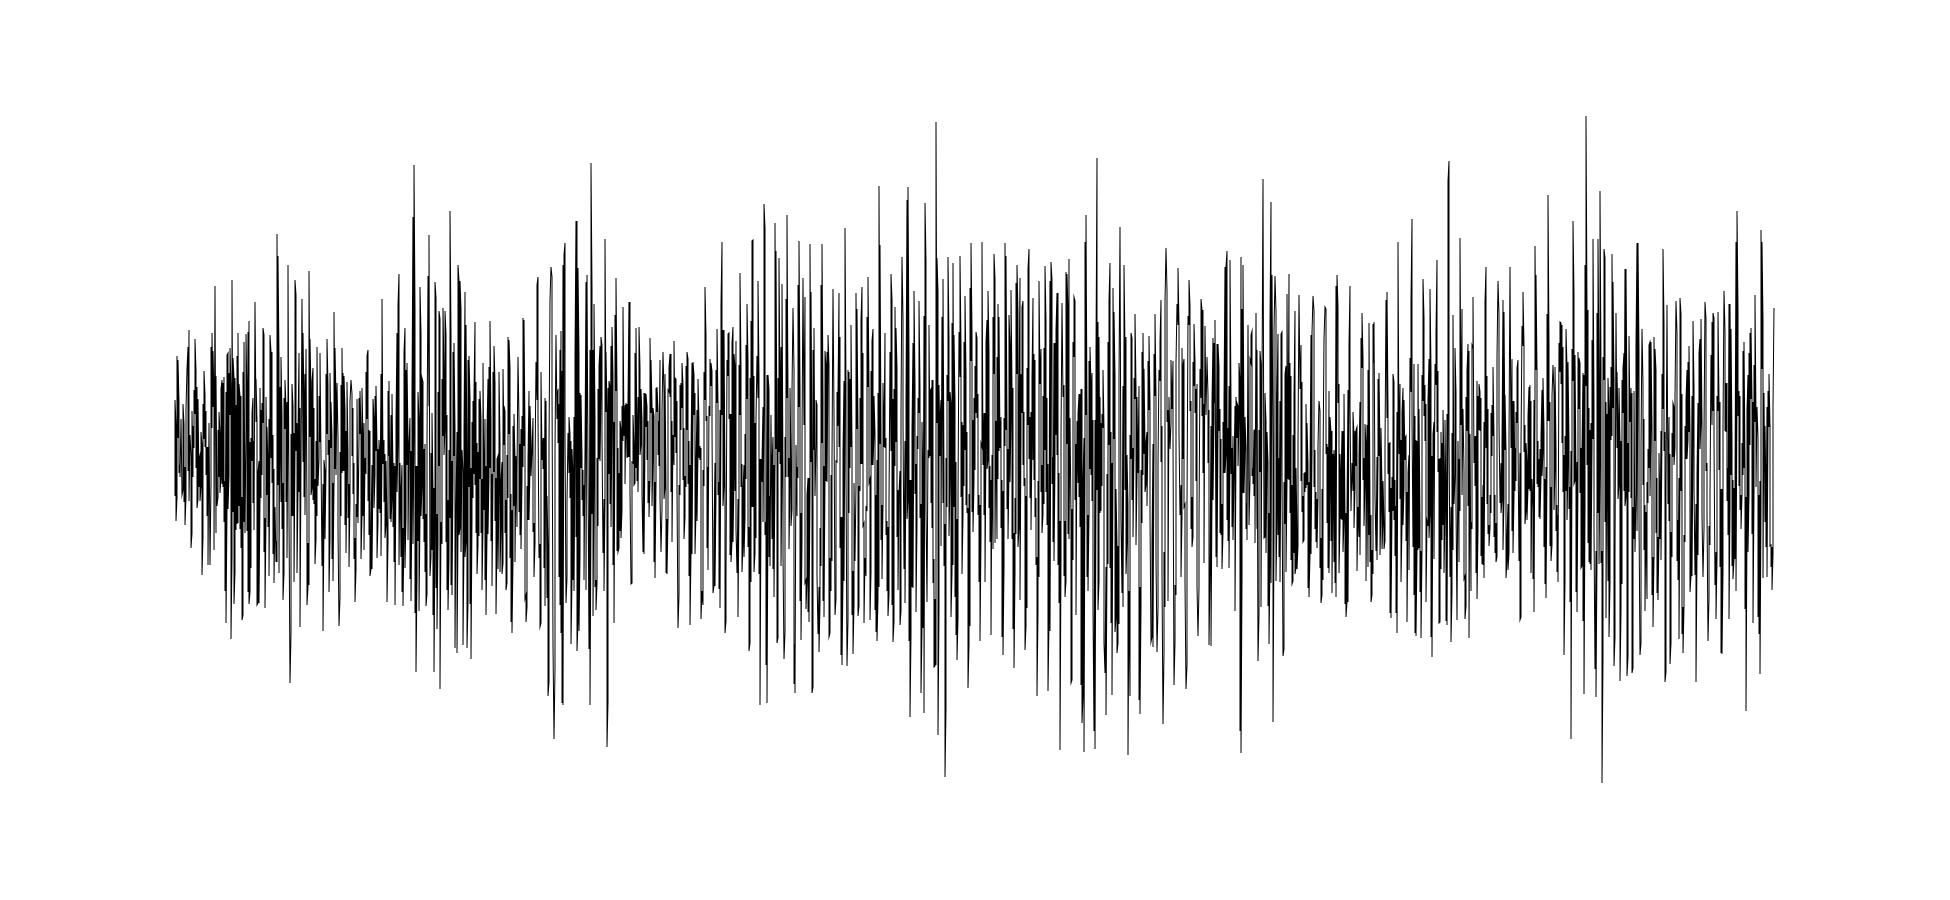
\includegraphics[width=0.45\textwidth]{figure/single-channel-animals.png}
%   \caption{A waveform graph representing the high and low pressure fluctuations that comprise sound.}
%   \label{fig:waveform}
% \end{wrapfigure}

While there are more than 30 years of research involving ASR, and nearly as many working with speech in noisy environments, it is impossible to touch on all techniques in this very brief overview.  Therefore, only several areas of research in noise-robust ASR will be discussed pertaining to the present research.

Equation \ref{eq:basic} is often used to represent the combination of speech and noise,
\begin{equation}\label{eq:basic}
y = x * h + n
\end{equation}
where $x$ is the clean speech signal, $h$ is any convolution (ie. room reverberation, microphone channel warp), $n$ is additive noise, and $y$ is the noisy speech signal.  There is also the effect that phase plays on the combination of the parts of this equation.  Taking phase into account means that additive noise is not always simply additive, as energy at frequencies with competing phases could cancel each other out at varying degrees, depending on phase.  While there is some research that does take phase into account and demonstrates that by doing so, greater noise removal can be acheived, attempting to model phase adds significant complexity, and the, albeit (many researchers in this subfield admit) problematic, assumption is made that phase plays no role.  

%Multi-style training, what it is (training with multiple types of noise) - it is ineffective.  Older - paper cited was written in 1987. \cite{li:14}, \cite{lippmann:87}.

It is difficult to categorize the plethora of noise-robustness techniques utilized by hundreds of researchers over the years, but, broadly, two domains can be discerned (\cite{li:14,zhang:17}).  The first is the ``feature-space'' domain, which focuses on front-end processing of the signal $y$ itself.  The second group utilizes the ``model space'' domain, or the back-end processing that modifies the acoustic model itself to account for any noise in the signal $y$.  Advances in neural network technology has also lent itself to application in noise-robust ASR.  These have provided novel methods of tackling the problem.

\subsection{Feature Space Domain vs Model Space Domain}

Feature space is the part of the ASR process where an acoustic vector is transformed into `features' about the acoustic signal that the ASR model will receive as input.  Model space, imperatively, then, comes after Feature space in the ASR process, and encompasses the acoustic model parameters, methods of training the model, etc.

Noise can be accounted for in either or both domains.  In the feature domain, noise is dealt with prior to the sending the features to the acoustic model.  These noise reduction processes intend to enhance the signal before it reaches the model.  This is mostly done without altering the acoustic model parameters, resulting in low computation cost.

In the model space, acoustic parameters themselves can be modified in accordance with the noisy signal.  This generally results in high computation cost when training the acoustic model.  There is normally a trade-off of computation and performance, with Model Domain space alterations generally yielding higher performance improvement (\cite{li:14}).

In the feature domain space, there are a number of techniques, including (a) noise-resistant features, (b) feature normalization, and  (c) feature compensation.  Noise resistant features are, quite simply, features in the acoustic signal which are not sensitive to environmental changes.  Many methods of deriving these features have been proposed that incorporate features of the human auditory system, including Perceptual Linear Prediction (PLP, \cite{hermansky:85}), which introduces the ``auditory spectrum'' and explicit F1/F2 information into ASR processing, and Relative Spectral processing (RASTA) applied to PLP (\cite{hermansky:92}), making PLP less sensitive to slow varying speech information, and more sensitive to the quick-varying transitions of speech (\cite{story:10}).  \cite{kim:99} attempts to model functions of the cochlea and auditory nerve. These methods are quite effective at dealing with short-term, stationary, additive noise (\cite{zhang:17}).  More recent methods include SPARK (\cite{fazel:12}, 1369), which is ``neurobiologically inspired'' by ``auditory receptive fields'' and ``local competative behavior'', and \cite{moritz:15}, which emulates the amplitude modulation found in mamillian auditory cortexes.  These methods generally outperform vanilla MFCC methods. Difficulties utilizing these methods include that the features can be quite complex to generate and the parameters difficult to set, preventing widespread usage with other techniques.  Due to the complexity involved, it is also difficult to derive a relation between clean and noisy speech \cite{li:14}.

Feature normalization generally involves normalizing cepstral feature vectors in the form of cepstral mean normalization (CMN) and cepstral mean and variance normalization (CMVN).  CMN invovles finding the mean values out of all cepstral vectors (\cite{atal:74}).  All cepstral vectors are then normalized, such that the mean cepstral value becomes zero.  This is primarily used to eliminate reverberation and channel-related distortion, but signals with noise and no channel distortion also see improvement (\cite{droppo:08}).  ``CMVN normalizes the mean and covariance together'' (\cite{li:14}, 752), yielding improved performance on speech data with additive noise.
These methods do not work in real-time, however, as they require cepstral vectors from the entire utterance in order to calculate a mean.

Feature compensation actually attempts to remove the noise from the noisy speech signal, allowing for use of traditional features. Spectral subtraction (\cite{boll:79} is an older and intuitive method of removing noise by turning the linear signal into the spectral domain, subtracting a noise spectrum from a noisy speech spectrum, leaving the clean speech spectrum.  This is then converted back into the series of samples that derive the clean speech spectrum.  This is performed all along the waveform.  The noise can be estimated by looking at sections of the observed signal that do not contain speech information.  

This method still comes with several problems (\cite{li:14}). First and foremost, it is difficult to detect the location of speech in the signal in a noisy environment, which consequently affects the ability to accurately compute a noise average. It also requires relatively stationary, slow-variation noise, as noise that changes quickly very possibly has a different average spectrum during the portion of the signal containing speech than the portion of the signal in which it was calculated.  Furthermore, this is only an average of the noise, and not exactly the noise itself; this subtraction can inadvertently have an additive noise effect by producing extraneous acoustic artifacts in the ``clean'' signal which were not there to begin with (\cite{berouti:79})

Weiner filtering (\cite{weiner:79}) is another method used to remove noise from a signal.  As opposed to spectral subtraction, however, this is a linear filter that works without the need to convert the signal into spectra.  However, this method also requires an estimation of the noise.  Furthermore, it does not do well in very low SNR enviroments, as it generally results in suppression and dampening of the entire signal (\cite{li:14}).

More standard, is the ``advanced front-end'' (AFE) ensemble proposed in \cite{etsi:02}.  It yields more than 50\% improvement over standard MFCC features alone, and has become a frequent baseline for comparison in noisy ASR research.  It is composed of three separate `tools': two stage Mel-warped Weiner filtering, SNR-dependant waveform processing, and blind equalization (cf. \cite{argawal:99,macho:02;macho:01;mauuary:98}, respectively.


Most of the heavy work is performed by the Mel-warped Weiner filtering (\cite{li:14}).  This differs from the more standard Weiner filter in that it uses the Mel-frequency power spectrum in the Weiner filter calculations, the result of which is then converted back into the time domain.  The filter is applied once, and then a second time to remove residual noise.  SNR-dependant waveform processing (SDWP) assumes that the noise is relatively constant, whereas the speech signal will cause variation in the amplitude of the signal.  SDWP uses this assumption to dampen portions of the signal with a relatively low SNR (ie, speech-less) compared with the high SNR (ie, speech-bearing) portions of the signal, which are boosted.  Blind equalization serves to eliminate convolutional (ie. reverberant) distortion from the signal.



Not much time will be spent describing existing model space domain compensation techniques, as this is not the focus of the present study.  This form of compensation usually involves adapting an existing acoustic model (presumably trained on relatively clean speech) to enable recognition of more noisy features.  Most popularly, variations of maximum likelihood linear regression (MLLR, \cite{leggetter:95}) are used to adjust the gaussian component vector means and the covariance parameters to account for differences in the signal that noise introduces.  A slight variation in the caculation allows these transforms to be applied to the features themselves (feature-space MLLR, or fMLLR, \cite{gales:98}), moving this method into an on-line feature space tranformation.  There has also been increasing research that combines the modification of features with the training of the acoustic model, called joint model training.  Broadly, this uses the acoustic features modified by techniques such as those described above within the training data for building the acoustic model.



% Another tool used is the exploitation of any prior knowledge about the distortion (\cite{li:14}); this is prior knowledge that is utilized during the training stage, not knowledge about the noise during the testing stage.  Some methods include learning the mapping between noisy and non-noisy pairs of acoustic signals.  This mapping is then extended to novel noisy utterances during testing.  This is used in feature domain space to enhance a noisy speech feature to then send to the model.  
% 
% Other methods utilze mutliple acoustic models, each trained on data from different environments and different noises and different SNRs.  The means and covariance matrices of each of these models are stored, and during recognition, the most appropriate model is chosen to use to decode the signal in question.  Either of these tactics, though, do require prior knowledge about the noise.  As with multi-style training, explained above, it is very difficult to ensure that all noises, SNRs, etc, are adequately accounted for during training in order to be prepared for what is seen during testing.
% 
% 
% %Implicit vs Explicit Distortion Modelling
% 
% Explicit distortion modelling uses a ``physical model'' which allows for high performance with few distortion parameters. An example of an explicit distortion model would be spectral subtraction, discussed earlier.  It seems obvious that spectral subtraction, when matched with an agreeable signal that best utilizes its noise removal abilities, would result in more accurate speech recognition.  Consequently, other noise reduction methods that \textit{explicitly} specify the distortion tend to perform well.


[\textbf{Read \cite{paliwal:12}, find out where to put it in above discussion, introduces MMSE (minimum mean square error). \cite{zhang:17}, 4 that it is still considered to be the best ``general purpose'' noise-removal tool.}]

% \textbf{For examples of what this distortion model actually is, go to the primary literature:}
% Y. Zhao and B. H. Juang, “A comparative study of noise estimation
% algorithms for VTS-based robust speech recognition,” in
% Proc. Inter-
% speech
% , 2010, pp. 2090–2093.
% J.Li,L.Deng,D.Yu,Y.Gong,
% andA.Acero,“Hi
% gh-performance
% HMM adaptation with joint compensation of additive and convolutive
% distortions via vector Taylor series,” in
% Proc. ASRU
% , 2007, pp. 65–70.
% [132] J.Li,L.Deng,D.Yu,Y.Gong,andA.Acero,“Auni
% fi
% ed framework of
% HMM adaptation with joint compensation of additive and convolutive
% distortions,”
% Comput., Speech, Lang.
% , vol. 23, no. 3, pp. 389–405, 2009.

There are two primary categories of utilizing neural networks to account for noisy speech, ``mapping methods'' and ``masking methods''.  Mapping methods primarily fall underneath the umbrella of feature-space methods.  This involves finding the non-linear function that maps the noisy speech to the clean speech.  In neural network terms, the noisy speech is the input to some type of neural network (eg. DNN, CNN, RNN, etc.) and the (intended) output is an approximation of the clean speech.  Due to the complexity of speech in the temporal domain, the input to the neural network usually comes from one of the later input transformations, such as from the spectral or cepstral domains (\cite{zhang:17}).

Masking-based approaches work similarly to a traditional filter, albeit learned via a neural network. These are also performed as a feature-space tool.  An `Ideal Ratio Mask' will learn the ratio (value between 0 and 1) of the clean speech to the noisy speech.  The function can be learned - via an neural network architecture - between the noisy speech signal and the masking value.  Most beneficial when using spectral or cepstral features as input, a masking value is learned for each set of features.  These masking values are then multiplied elementwise to each feature in the set, at that time index within the signal, ie. a method very similar to that of a traditional filter (\cite{zhang:17}).

There are also a few model-based approaches using neural networks for noise robust ASR.  Most widely used is multi-condition training (\cite{seltzer:13,zhang:17}, which, similar to multi-style training originally developed by \cite{lippmann:87}, uses an collection of training data which exhibits a wide range of noise conditions.  Another method, similar to methods used in non-neural network approaches, involves adapting the already trained acoustic model with a small subset of noisy data.  However, as doing so can inadvertently result in significant overfitting, \cite{mirsamadi:15} has developed a technique unique to neural networks that - instead of slightly adjusting all weights, adds an additional layer to the neural network with its own weights, instead of modifying all weights.  This largely avoids the issue of overfitting, while increasing the model's robustness to noise.

Much work is also turning to combine modifications in the feature space domain, with modififications in the model space domain (\cite{weninger:13}).  Most simply, this takes the form of using the feature-enhanced data output from feature-based noise removal as training data itself for the acoustic model.


There are also techniques that employ multiple microphones as source-separation technique to separate the speech source from any extraneous noise sources.  The study at hand does not use multiple microphones, and so this will be discusses as only a reference.  Beamforming (\cite{veen:88}) has become a central technique to using microphone arrays in source separation (\cite{hori:15,zhang:17}).
This is done by calculating the direction of arrival of the different sound sources, taking into account the distance between the two (or more) microphones, and the time of arrival of the different sources in each signal recorded by the microphone.  Neural networks have also been employed to aid and enhance the beamforming process (\cite{heyman:15,sivasankaran:15,heyman:16}).  




% For noise-robust ASR utilizing multiple microphones, refer to any of the following:
% T.Virtanen,R.Singh,andB.Raj
% , Techniques for noise robustness in
% automatic speech recognition
% .  New York, NY, USA: Wiley, 2012. OR
% 
% [31] S. Makino, T.-W. Lee, and H. Sawada
% , Blind Speech Separation
% .
% New York, NY, USA: Springer, 2007.
% [32] J. Benesty, M. M. Sondhi, and Y. Huang
% , Springer Handbook of Speech
% Processing
% .  New York, NY, USA: Springer, 2007.
% [33] P. A. Naylor and N. D. Gaubitch
% , Speech Dereverberation
% .New
% York, NY, USA: Springer, 2010.
% 
% ALSO
% 
% [41] T. Yoshioka and T. Nakatani, “Noise model transfer: Novel approach
% to robustness against nonstationary noise,”
% IEEE Trans. Audio, Speech,
% Lang. Process.
% , vol. 21, no. 10, pp. 2182–2192, Oct. 2013
% 
% AND
% 
% [42] M.Souden,S.Araki,K.Kinoshita,T.Nakatani,andH.Sawada,“A
% multichannel mmse-based framework for speech source separation and
% noise reduction,”
% IEEE Trans. Audio, Speech, Lang. Process.
% ,vol.21,
% no. 9, pp. 1913–1928, Sep. 2013.





\section{Experiment 2: ASR of Ear-Recorded and Noisy Mouth-Recorded Speech}

While there are many proposed techniques, discussed in Section \ref{chap3:background}, that have been used to modify the acoustic features of noisy speech, or to modify the acoustic model to compensate for noise, noise-robust ASR is still imperfect, and requires additional advances to ASR technology (\cite{zhang:17}).  This particular study proposes the new technique of using speech recorded from the inside of the ear canal.  This would be classified as a feature space modification in the temporal domain, prior to any processing.  Rather than using significant computation to acheive the noise reduction, this study employs purely passive mechanisms (ie. tissues in the head, earplug, ear muffs) to reduce noise.  

As described previously in Chapter 2\ref{chapter2}, very simple signal enhancement techniques (ie. pre-emphasis and band-pass filtering)\footnote{These are simple enough to be built into an electrical chip to be performed in real-time, requiring no actual computation.} are then applied to the recorded signal to produce an enhanced signal with relatively little noise and one that is very similar to what could be recorded at the mouth (below 2.7 kHz).

\subsection{Stimuli}

Recordings from twenty speakers, ten male and ten female, from the data collection experiment in Chapter 2\ref{chapter2} were used as test data for this experiment.  This included 30 distint sentences from each speaker, each with 5 different noise conditions (bus, cafe, pedestrian, street, factory), 3 different noise levels (60dB, 70dB, 80dB), and a `clean' (no noise) condition.  This results in 16 iterations of each distict sentence, for each speaker, totalling 480 sentences per speaker, 4800 sentences for each gender group, and 9600 total test sentences.

\subsection{Design}

The existing \textbf{OPEN SLR} acoustic model will be used to test the collected data.  \textbf{This acoustic model has not been trained on significantly noisy data}.  This will primarily test the performance between the ear-recorded and noisy mouth-recorded speech, but also between the different noise conditions and noise levels.  Both the ear-recorded and noisy mouth data will then be enhanced using the well-established advanced front end (AFE, \cite{etsi:02}) technique, and will be retested on the same, unchanged acoustic model.

It is quite possible that, due to the ear-recorded speech only containing information below 3 kHz, that the existing acoustic model in its current state will have poor recognition of these sentences.  If this is the case, the same acoustic model will be adapted with ear-recorded and low-pass filtered additional setnences (not from the 30 test sentences, nor from any of the speakers being tested).  A total of \textbf{XXX} distinct sentences from \textbf{XX} additional speakers were used for adaptation of the acoustic model, totalling \textbf{XXX} sentences used for adaptaiton.  The same 9600 sentences from the same 20 speakers were used again for test data.

\subsection{Procedure}

\subsection{Results}

\section{Discussion}

\subsection{Limitations and Future Research}

This study utilized noise that was by and large stationary in amplitude.  This was intentional, to test the proof of concept and to test the extent (amplitude) of noise the proposed method can handle.  In theory, as has been shown in Chapter 2\ref{chapter2} that the noise does not have a dramatic effect on speech recorded from the ear, variations and modulations in the amplitude of the noise (and hence the SNR of the speech recorded at the mouth) should have no effect on the speech recorded at the ear.  Nevertheless, this should be investigated.  The recent CHiME Challenge (2016) has incorporated amplitude varying noise into their task, and similar tests could be performed by collecting another data set of speech recorded from participants' ears, with amplitude varying noise.




\bibliographystyle{apa}
\bibliography{DissRefs.bib}
\end{document}

\documentclass[dissertation,copyright]{uathesis}
\usepackage[]{graphicx}\usepackage[]{color}
%% maxwidth is the original width if it is less than linewidth
%% otherwise use linewidth (to make sure the graphics do not exceed the margin)
\makeatletter
\def\maxwidth{ %
  \ifdim\Gin@nat@width>\linewidth
    \linewidth
  \else
    \Gin@nat@width
  \fi
}
\makeatother

\definecolor{fgcolor}{rgb}{0.345, 0.345, 0.345}
\newcommand{\hlnum}[1]{\textcolor[rgb]{0.686,0.059,0.569}{#1}}%
\newcommand{\hlstr}[1]{\textcolor[rgb]{0.192,0.494,0.8}{#1}}%
\newcommand{\hlcom}[1]{\textcolor[rgb]{0.678,0.584,0.686}{\textit{#1}}}%
\newcommand{\hlopt}[1]{\textcolor[rgb]{0,0,0}{#1}}%
\newcommand{\hlstd}[1]{\textcolor[rgb]{0.345,0.345,0.345}{#1}}%
\newcommand{\hlkwa}[1]{\textcolor[rgb]{0.161,0.373,0.58}{\textbf{#1}}}%
\newcommand{\hlkwb}[1]{\textcolor[rgb]{0.69,0.353,0.396}{#1}}%
\newcommand{\hlkwc}[1]{\textcolor[rgb]{0.333,0.667,0.333}{#1}}%
\newcommand{\hlkwd}[1]{\textcolor[rgb]{0.737,0.353,0.396}{\textbf{#1}}}%
\let\hlipl\hlkwb

\usepackage{framed}
\makeatletter
\newenvironment{kframe}{%
 \def\at@end@of@kframe{}%
 \ifinner\ifhmode%
  \def\at@end@of@kframe{\end{minipage}}%
  \begin{minipage}{\columnwidth}%
 \fi\fi%
 \def\FrameCommand##1{\hskip\@totalleftmargin \hskip-\fboxsep
 \colorbox{shadecolor}{##1}\hskip-\fboxsep
     % There is no \\@totalrightmargin, so:
     \hskip-\linewidth \hskip-\@totalleftmargin \hskip\columnwidth}%
 \MakeFramed {\advance\hsize-\width
   \@totalleftmargin\z@ \linewidth\hsize
   \@setminipage}}%
 {\par\unskip\endMakeFramed%
 \at@end@of@kframe}
\makeatother

\definecolor{shadecolor}{rgb}{.97, .97, .97}
\definecolor{messagecolor}{rgb}{0, 0, 0}
\definecolor{warningcolor}{rgb}{1, 0, 1}
\definecolor{errorcolor}{rgb}{1, 0, 0}
\newenvironment{knitrout}{}{} % an empty environment to be redefined in TeX

\usepackage{alltt}
\newcommand{\SweaveOpts}[1]{}  % do not interfere with LaTeX
\newcommand{\SweaveInput}[1]{} % because they are not real TeX commands
\newcommand{\Sexpr}[1]{}       % will only be parsed by R


%\documentclass[dissertation,CC-BY]{uathesis}
%\documentclass[dissertation,CC-BY-SA]{uathesis}
%documentclass[dissertation,CC-BY-ND]{uathesis}
%\documentclass[thesis]{uathesis}
%\documentclass[document]{uathesis}

% Package Usage
% These are the packages that we need
\usepackage{booktabs}
\usepackage{graphicx}
\usepackage{natbib}			% natbib is available on most systems, and is
					% terribly handy.
					
%May need to remove! Trying to fix nocite{*} biblography problem:
					% If you want to use a different Bibliography package, 
					% you should be able to, just change this
					% and the \bibliographystyle command below.  Be warned
					% that you may need to do a little hacking to get
					% the REFERENCES item to show up in your TOC.

% Compatibility with the AASTEX package 
% of the American Astronomical Society.
%\usepackage{deluxetable}		% Allows use of AASTEX deluxe tables
%\usepackage{aastex_hack}		% Allows other AASTEX functionality.

% These are other packages that you might find useful.
% For controlling the fonts, see
% http://www.math.uiuc.edu/~hartke/computer/latex/survey/survey.html
% The following is a nice font set:
%\usepackage{mathtime}			% Times for letters; Belleek math.
%
\usepackage{wrapfig}

\newenvironment{lydiawrapfigure}
 {%
%  \setlength{\intextsep}{0pt}% <--- Wrong!
  \setlength{\columnsep}{15pt}%
  \wrapfloat{figure}%
 }
 {\endwrapfloat}
 
\usepackage{caption}
\usepackage{subcaption}
\usepackage{tipa}
\usepackage{color,soul}
\usepackage{url}
\usepackage{blindtext}
\usepackage[inline]{enumitem}
\usepackage{breakurl}
\usepackage{mathtools}
\usepackage{amsmath}
% \usepackage[normalem]{ulem}
% \usepackage{xyling,comment}			% AMS Math (advanced math typesetting)
% includecomment{delall}
% %\excludecomment{delall}
% 
% %default: don't show edits
% 
% \newcommand{\add}[1]{#1}
% \newcommand{\del}[1]{}
% \newcommand{\delni}[1]{}
% \newcommand{\addtab}{}
% 
% %block to show edits controlled by include/exclude-comment above
% \begin{delall}
% %added stuff
% \renewcommand{\add}[1]{\textcolor{blue}{#1}}
% %added table
% \renewcommand{\addtab}{\color{blue}}
% %deleted stuff
% \renewcommand{\del}[1]{\textcolor{red}{\sout{#1}}}
% \renewcommand{\delni}[1]{\noindent\textcolor{red}{\sout{#1}}}
% \end{delall}

%\usepackage{lscape}			% Used for making fitting large tables in by putting them landscape
%\usepackage{refs}			
%
% If you are using hyper-ref (recommended), this command must go after all 
% other package inclusions (from the hyperref package documentation).
% The purpose of hyperref is to make the PDF created extensively
% cross-referenced.

%Also works! Change dvips to driverfallback=dvips.
\usepackage[driverfallback=dvips,bookmarks,colorlinks=true,urlcolor=black,linkcolor=black,citecolor=black]{hyperref}


%Works!
%\usepackage[pdftex,bookmarks,colorlinks=true,urlcolor=black,linkcolor=black,citecolor=black]{hyperref}
%HERE IS THE THING THAT NEEDS TO CHANGE TO GET LATEX TO WORK WITH RSTUDIO. USE pdftex instead of dvips.

% Set up some values.
\completetitle{Working Title: An approach to automatic and human speech recognition using ear-recorded speech.}
\fullname{Samuel John Charles Johnston}			% Grad college wants your full name here.
\degreename{Doctor of Philosophy}	% Title of your degree.



\begin{document}
%set_parent(‘/Users/mwilli/Documents/Spring_2017/Dissertation_Document/Dissertation_Working_Directory_Draft/Dissertation_Main.Rnw')


 



\chapter{Human Speech Perception of Ear-Recorded speech\label{chapter4}}


\section{Introduction}

In order to judge the usefulness and intelligibility of the modified sounds recorded at the ear, it is necessary to run a human perception task on the recorded sounds.  Of primary interest is whether the speech recorded at the ear in a noisy condition (a) has resulted in a sufficient reduction in the ambient noise level, and (b) is markedly more intelligible that speech recorded at the \textit{mouth} in a noisy condition.

\section{Background}\label{chap2:background}

% I need to demonstrate:
%   - Explaining the acoustic structure of speech in noise
%   - Demonstrating why speech in noise is difficult for humans to understand (mechanically? neurologically?)
%   - Explain the average/expected performance of Humans when recognizing speech in noise
%   - Show the variability in ability to understand speech in noise by different speakers.
Human listeners' inability to understand a speech utterance can occur from an information loss that might be caused by any of a host of factors.  For example, information can be lost in the domain of time (eg. an intermittent signal), or from loss of intensity (eg. due to distance from the source), as well as the distortion of the source itself, such as a speech impediment (\cite{mattys:12}).  Of particular interest to the present study is the difficulty for human listeners to perfectly understand a speech signal due to additive background noise from sources other than the desired speech signal.

The ability of the human auditory system to hear and differentiate multiple sources of sound from a single pressure wave is often given the term ``auditory scene analysis'' (\cite{bregman:94}).  The term ``scene analysis'' is borrowed from the visual domain, implying the separation of a ``scene'' (be it auditory or visual) into its component objects (again, be they auditory or visual). For the purposes of this study, we will be discussing human auditory ability to find multiple sound sources from a temporal stream of air pressure fluctuations (ie. sound) reaching the tympanic membrane.

To visualize the auditory scene, note the waveform (ie. the graph of air pressure fluctuations) that reaches the tympanic membrane in Figure \ref{fig:animal_singlechannel}.  
%
\begin{wrapfigure}{r!}{0.5\textwidth}
\centering
  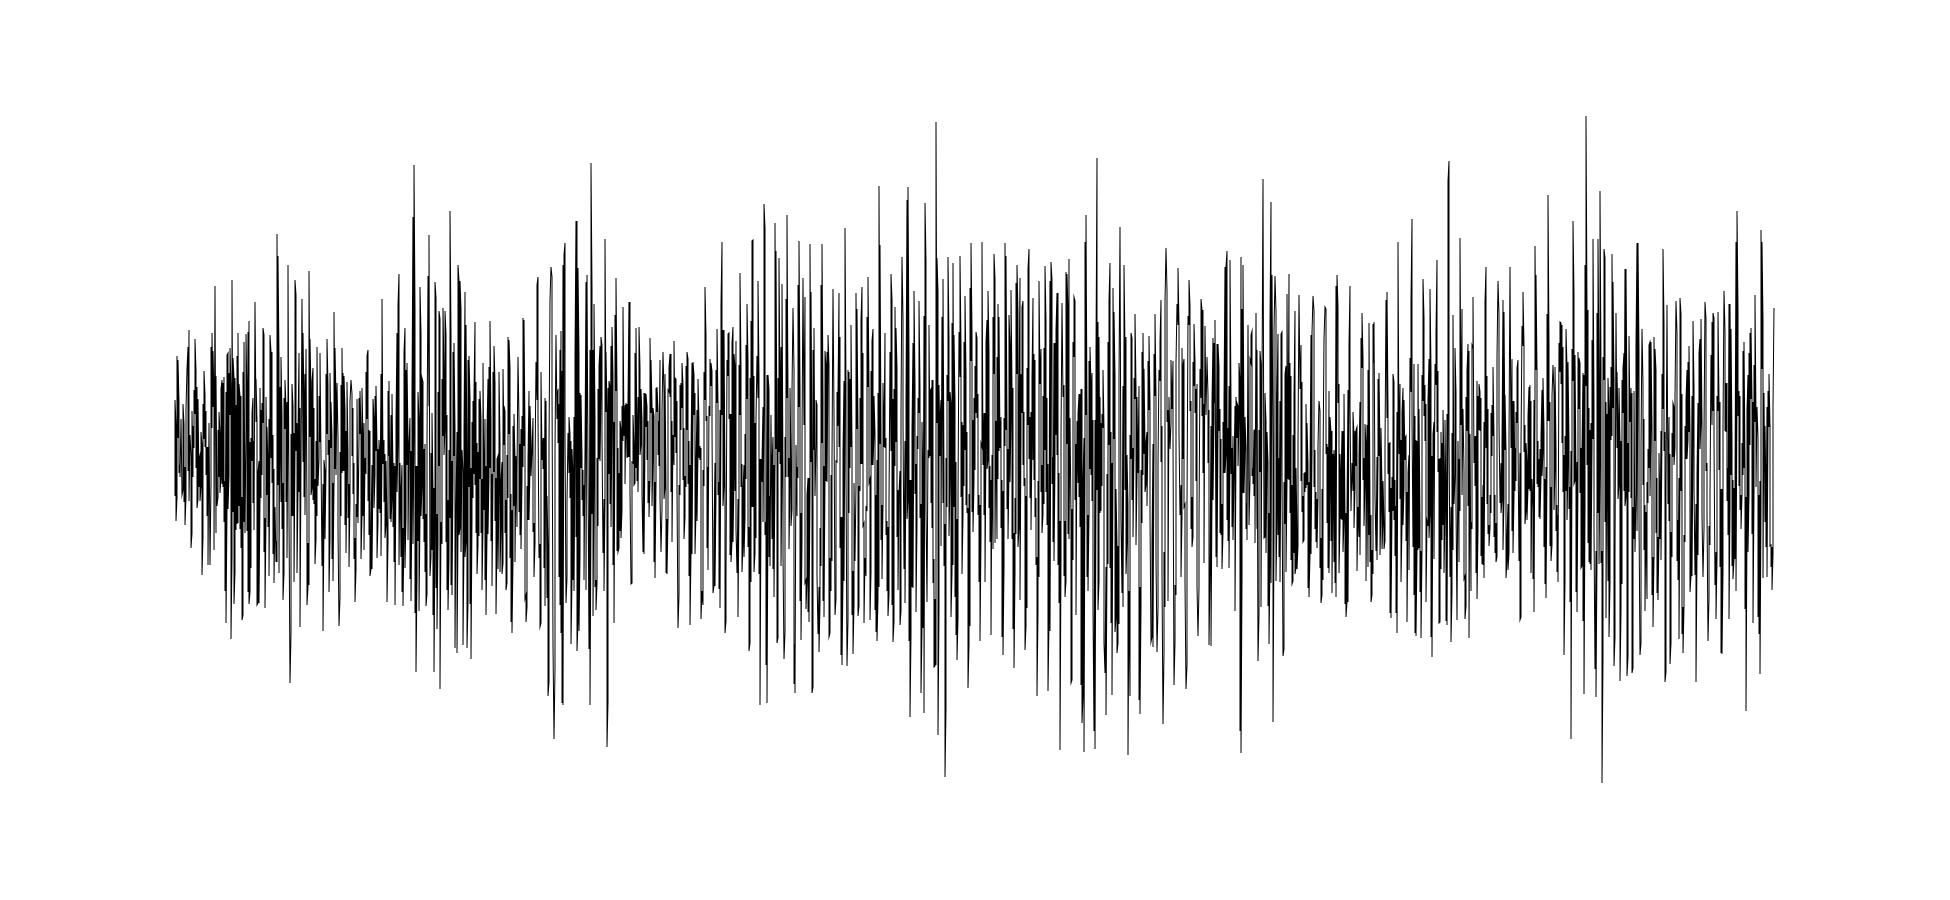
\includegraphics[width=0.45\textwidth]{figure/single-channel-animals.png}
  \caption{A waveform composed of multiple sound sources (cf. Fig. \ref{fig:animal_multichannel}).}
  \label{fig:animal_singlechannel}
\end{wrapfigure}
%
It is composed of all environmental sounds contributing to the air pressure fluctuation at the tympanic membrane\footnote{Note that this is for illustration purposes; the waveform will obviously look different when shaped by a given environment and the human ear canal before reaching the tympanic membrane.}.

However, using the framework of auditory scene analysis, the human auditory system is able to separate this input signal into its various sources, or ``auditory objects''.  In effect, this would separate the above waveform into its actual component sources of human speech, and the sounds of a sheep, cow, and horse, seen in Figure \ref{fig:animal_multichannel}; ``The normal auditory system exhibits a remarkable ability to parse these complex scenes'' (\cite{middlebrooks:17}, 2).

Of course, there reaches a point at which the auditory system fails and can
%
\begin{figure}[h]
\centering
  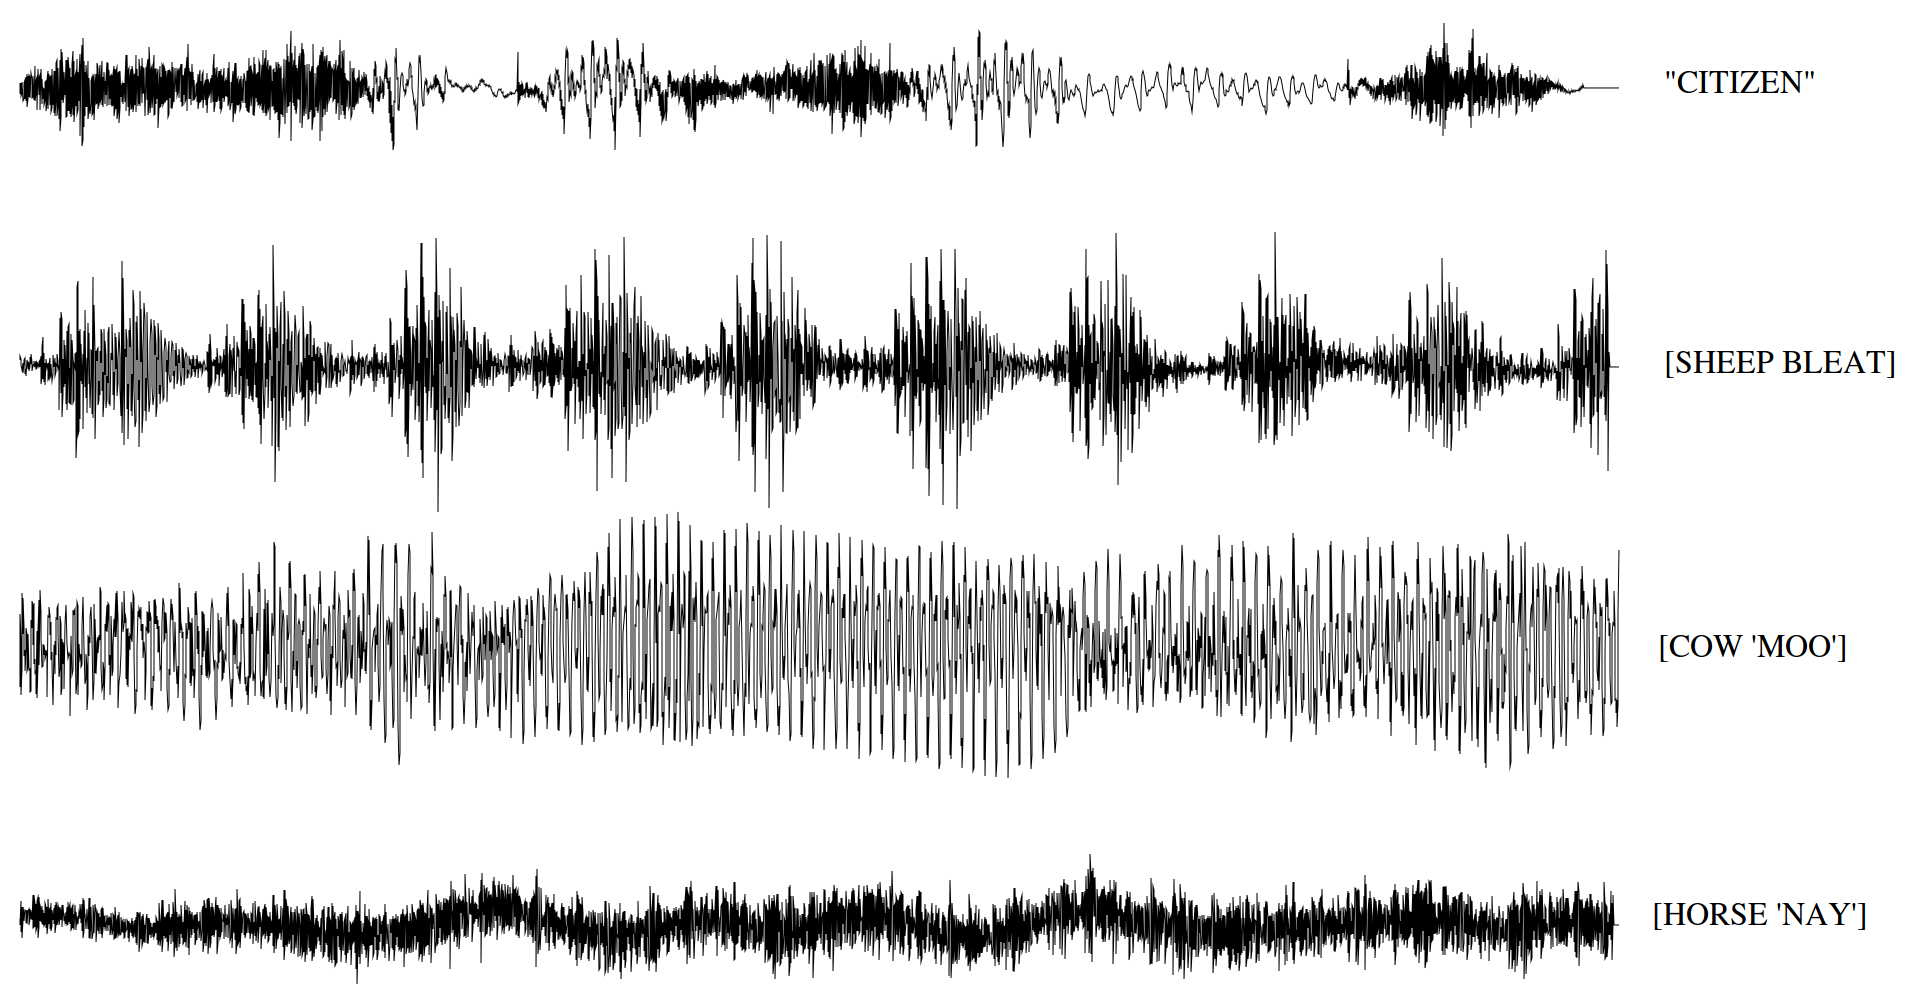
\includegraphics[width=0.95\textwidth]{figure/multi-channel-animals_w-text.png}
  \caption{The four component waveforms (human speech, sheep, cow, horse), of the combined waveform seen in Figure \ref{fig:animal_singlechannel}.}
  \label{fig:animal_multichannel}
\end{figure}
%
 no longer differentiate all sources, or, more relevant to this paper, recognize the information in a human speech signal when embedded with background noise from one or more additional sources.  The following section will describe in more depth the acoustics of speech in noise.
  
\subsection{Acoustics of Speech in Noise}
\label{bkgrnd:speech_in_noise}

Speech in noise can be intuitively grouped into two components, the speech (more specifically the voice one is intending to hear) and the noise, called the ``masking'' element.  Broadly, masking can be defined as ``the process by which the threshold of hearing for one sound is raised by the presence of another'' (\cite{ansi:13}, 61).  This masking element is anything \textit{but} the voice\footnote{For the purposes of this paper, the term ``voice'' will be used throughout to refer to the singular speech source the listener desires to hear out of the masked signal.} (speech signal) that one is interested in, as it was intended to be heard.
%which, as indicated in Chapter 2\ref{chapter2}, could be of any form or loudness.

The masking process can be broken down into two forms: energetic masking and informational masking.  Energetic masking occurs when the masking element shares the same temporal and frequency elements of the voice.  It can be thought of as if the masked element and the voice are competing for ``space'' along the basilar membrane and then the auditory nerve (\cite{brungart:01}), but can also be considered to be competing for the listener's attention (ie. the listener must concentrate on ignoring the mask, and exclusively listening to the target, (\cite{mattys:12})).  Energetic masking is normally thought to occur primarily in the ``lower'' auditory processes, eg. the cochlea and auditory nerve, though this is not always the case, as described further below.  

Informational masking can be broadly thought of as difficulties relating to memory, linguistic processing, and the like, oftentimes generalized to speech-on-speech noise.  \cite{mattys:10} failed to find informational masking in a cross-linguistic task, and so it is possible that informational masking could be limited to situations in which the masking speech is intelligible. This type of masking is thought to occur primarily in the ``higher auditory processes'' in the brain.

An instance of both energetic and informational masking can be visualized in a diagram of overlapping speech presented in \cite{middlebrooks:17}, and seen in Figure \ref{fig:sos-masked-spctgrms}.
%
\begin{figure}
\centering
  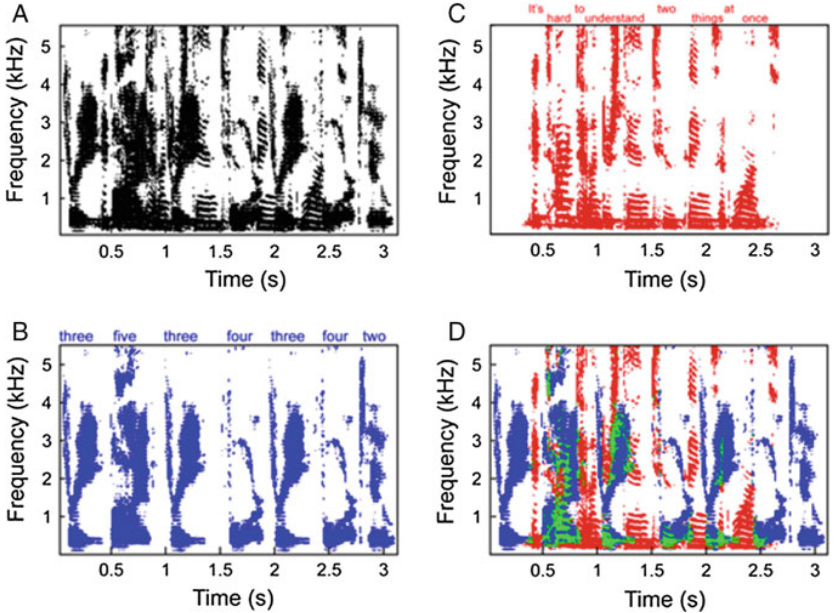
\includegraphics[width=0.95\textwidth]{figure/speech-on-speech_masked_spectrograms.png}
  \caption{Diagrams of different spectograms. (A) The spectogram of two temporally overlapping spoken utterances. (B) The spectogram of the utterance ``three five three four three four two'' colored in blue (C) The spectogram of the sentence ``It's hard to understand two things at once.'' colored in red. (D) The overlap of the two spectograms (B) and (C), with the color green highlighting the areas of energy in frequency and time that overlap. }
  \label{fig:sos-masked-spctgrms}
\end{figure}
%
Say that utterance (C) in the figure is the desired ``voice'', leaving utterance (B) the masking element.  In (D), one can see the voice (red), the areas of masking in which there is direct frequency and temporal overlap (green), and the remainder of the masking speech (blue). Of course this is never so nicely differentiated, and the resulting acoustic information that the auditory system gets can be seen in (A), in which no source is differentiated.  This could primarily be viewed as a form of energetic masking (competition for lower-level processing), though upper level processing is required to take meaning from the desired voice, which is masked informationally by the other, competing voice carrying its own information.

The five different background noises used in the study described in Chapter 2\ref{chapter2} primarily serve the purpose of energetic masking of the voice in the signal.  A small (5 second) portion of the spectrogram of each sound can be seen in Figure \ref{fig:bkgrnd-noises}.  These sounds don't produce any competing linguistic informational content themselves which mask the desired voice (the `caf\'{e}' noise, seen in Figure \ref{fig:cafe-bkgrnd}, does contain speech babble, none of it intelligible), and so masking occurs by producing energy at the same time as - and in the same frequency range as - the recorded voice.

\begin{figure}[h!]
\begin{subfigure}{0.475\linewidth}
  \centering
  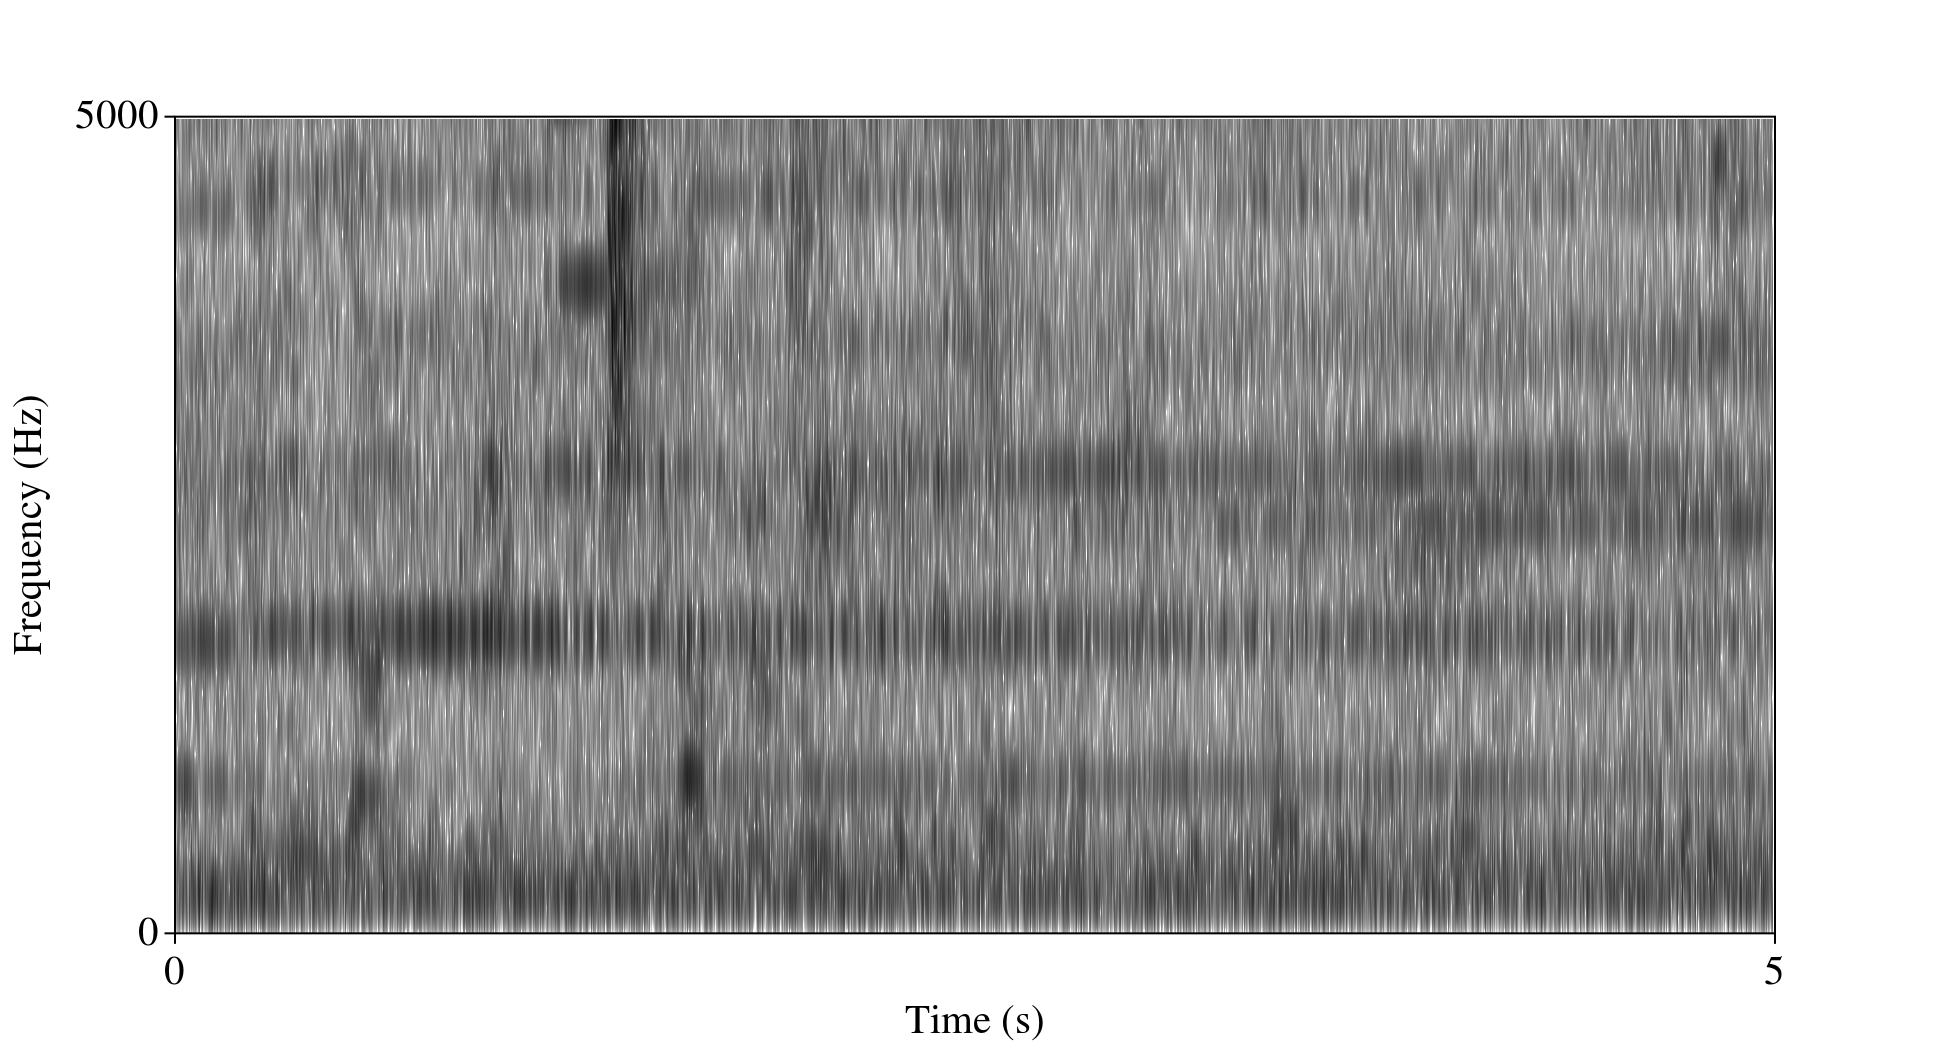
\includegraphics[width=0.9\textwidth]{figure/spctgrm-bus-background.png}
  \caption{Bus background noise.}
  \label{fig:bus-bkgrnd}
\end{subfigure}
\qquad
\begin{subfigure}{0.475\linewidth}
  \centering
  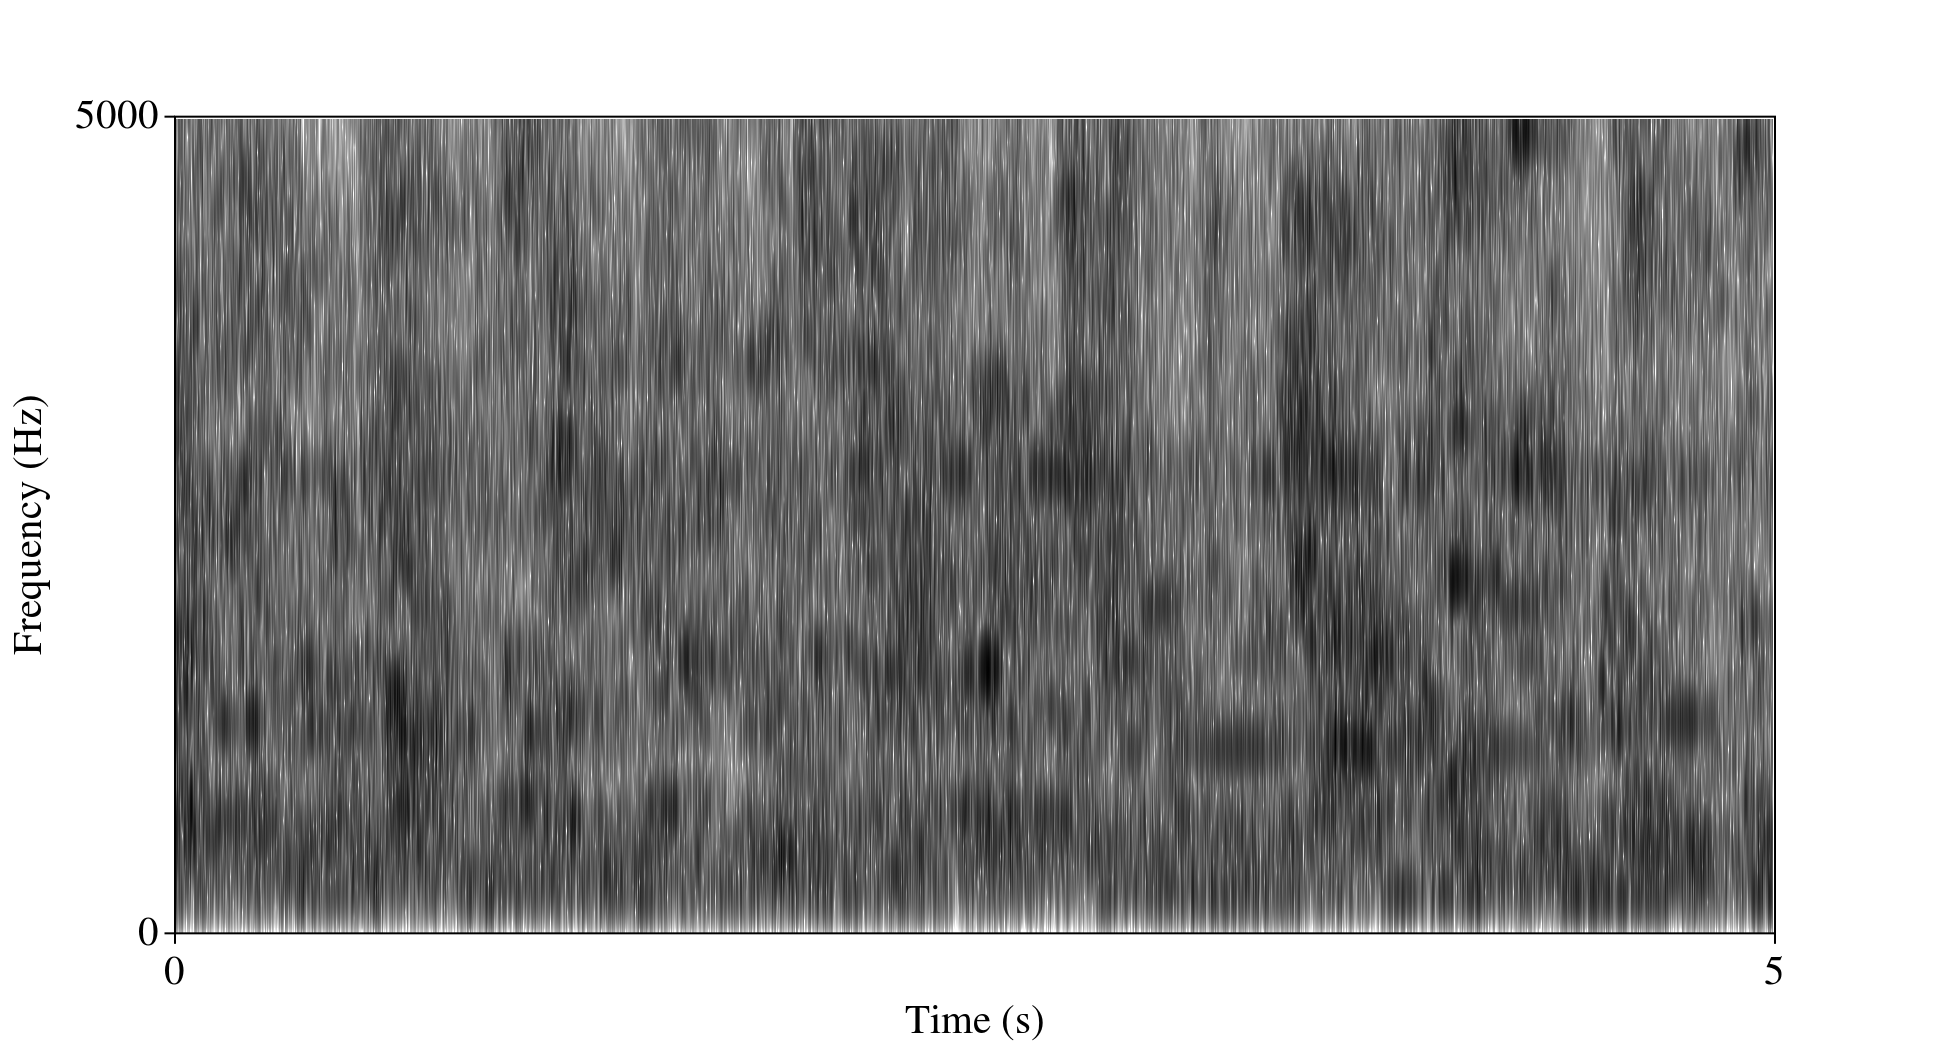
\includegraphics[width=0.9\textwidth]{figure/spctgrm-cafe-background.png}
  \caption{Caf\'{e} background noise.}
  \label{fig:cafe-bkgrnd}
\end{subfigure}%
%\hfill
\\[2ex]
\begin{subfigure}{0.475\linewidth}
  \centering
  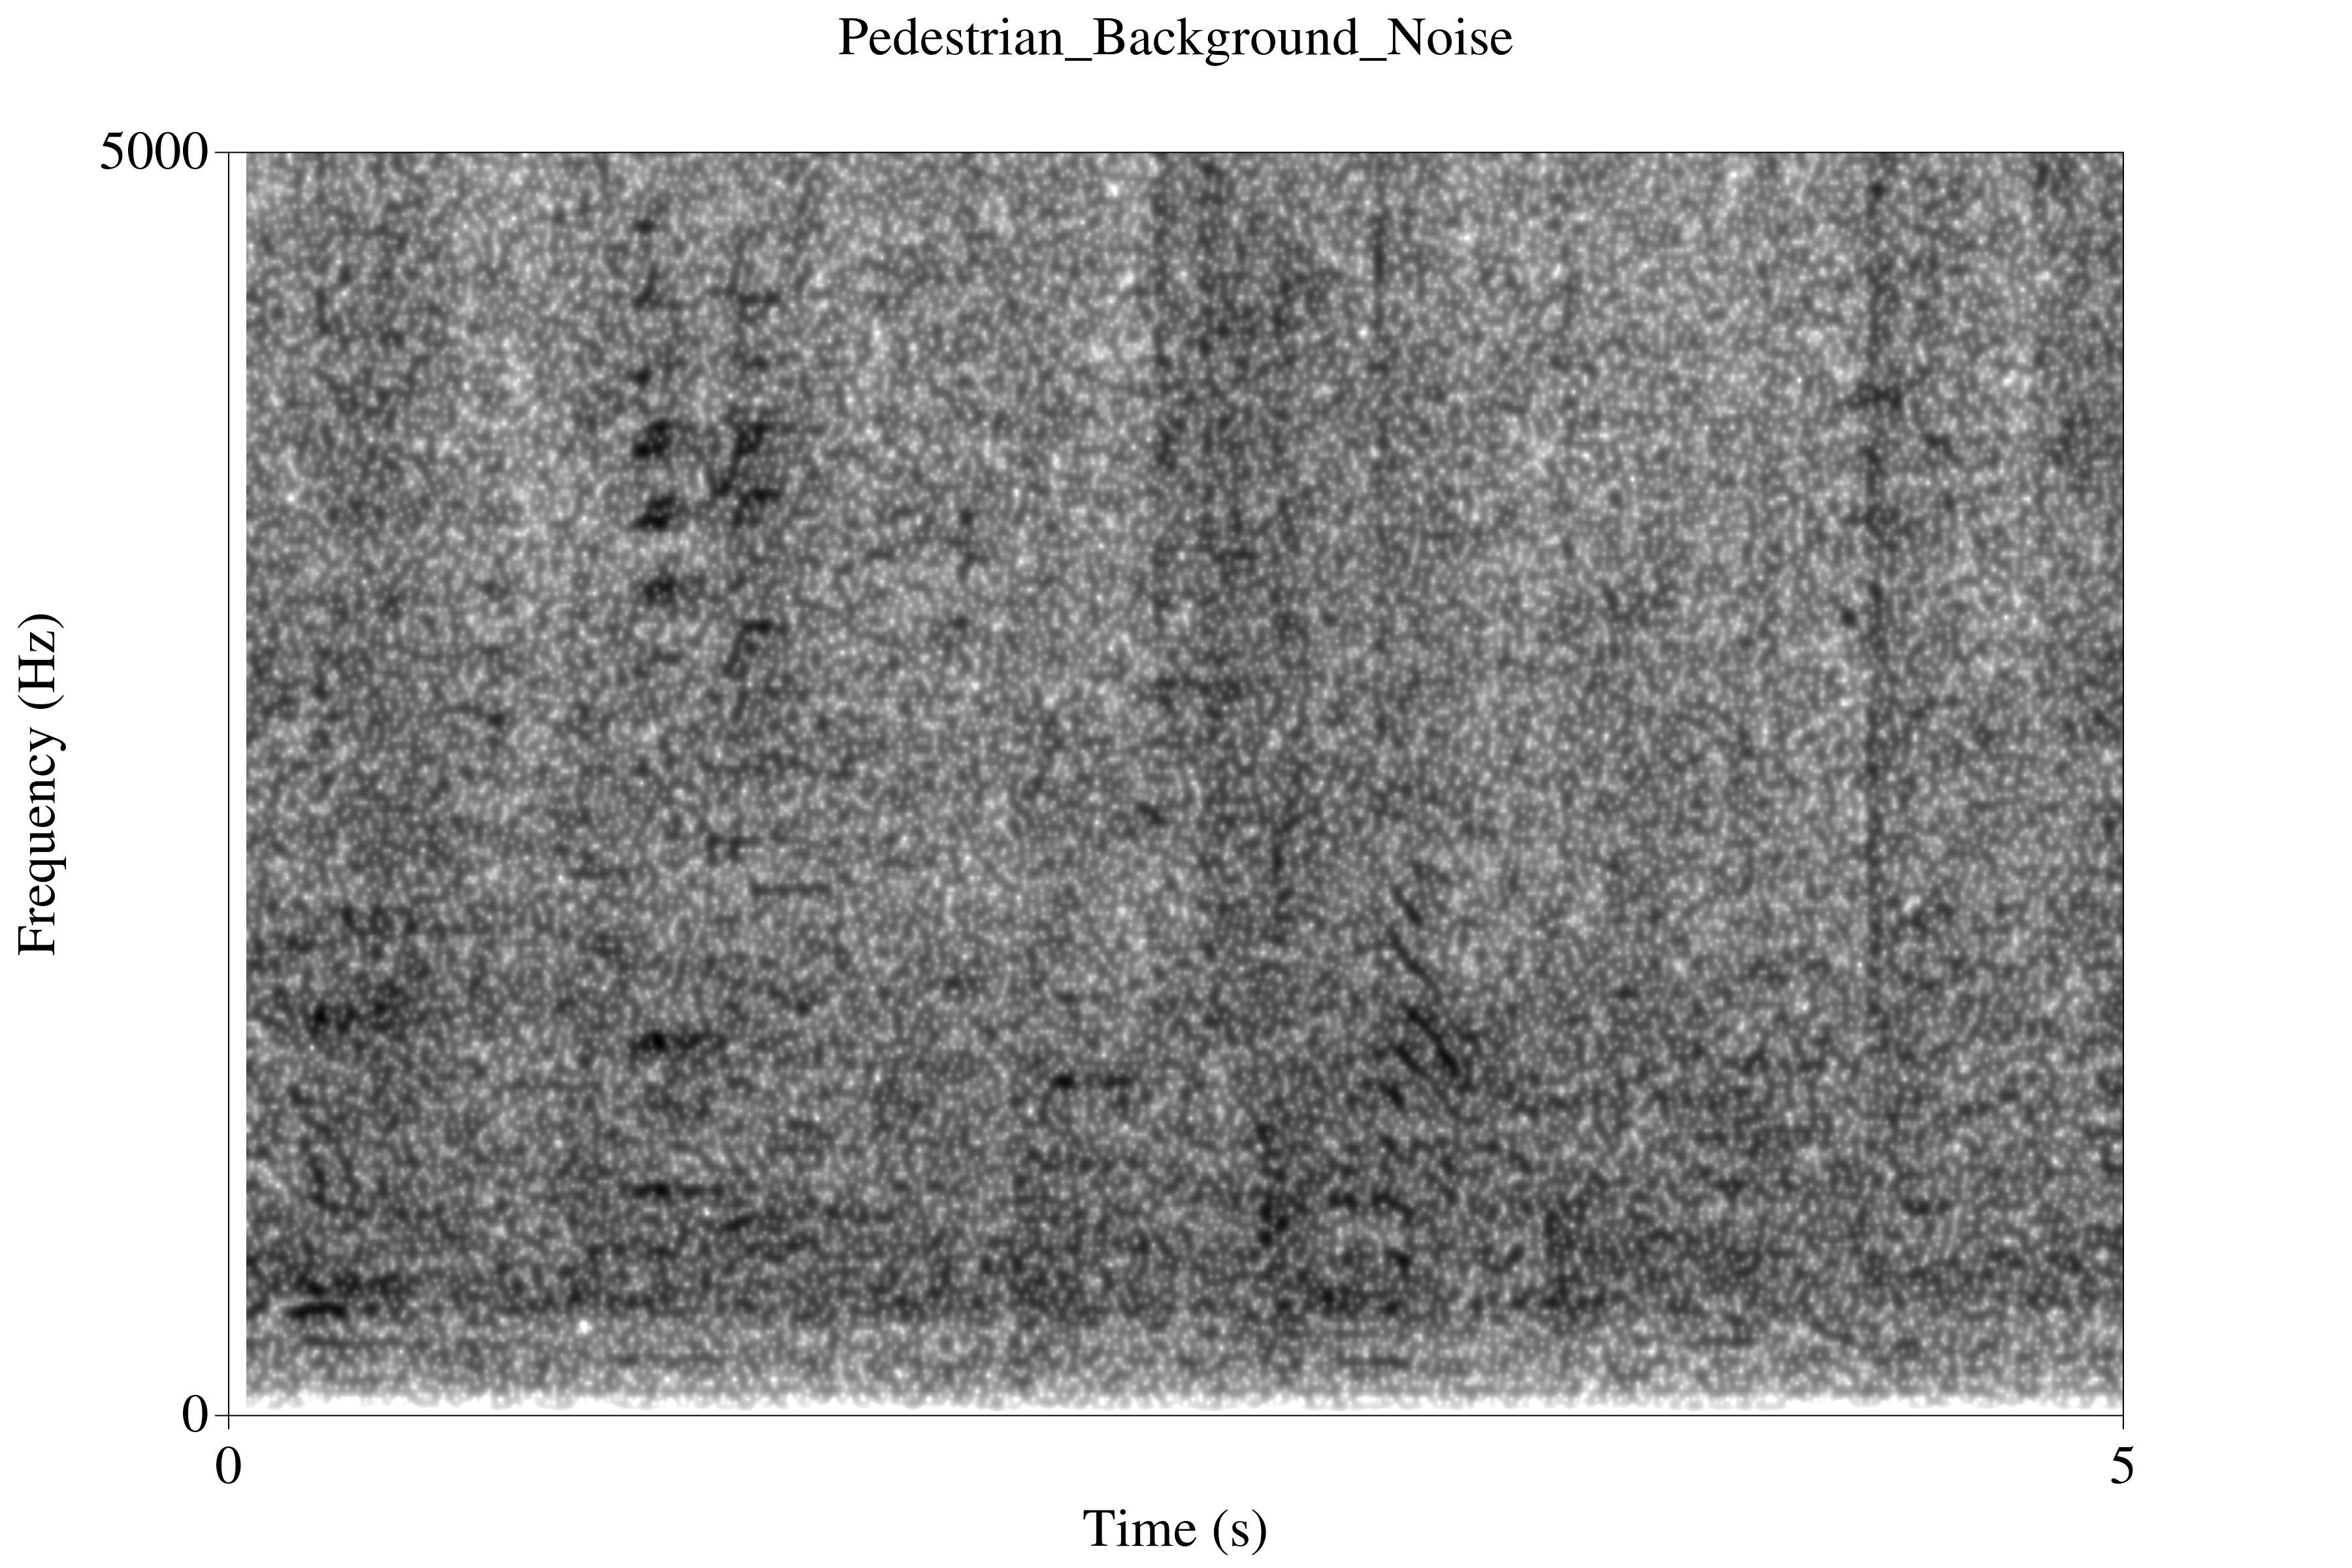
\includegraphics[width=0.9\textwidth]{figure/spctgrm-ped-background.png}
  \caption{Pedestrian background noise.}
  \label{fig:ped-bkgrnd}
\end{subfigure}
\qquad
\begin{subfigure}{0.475\linewidth}
  \centering
  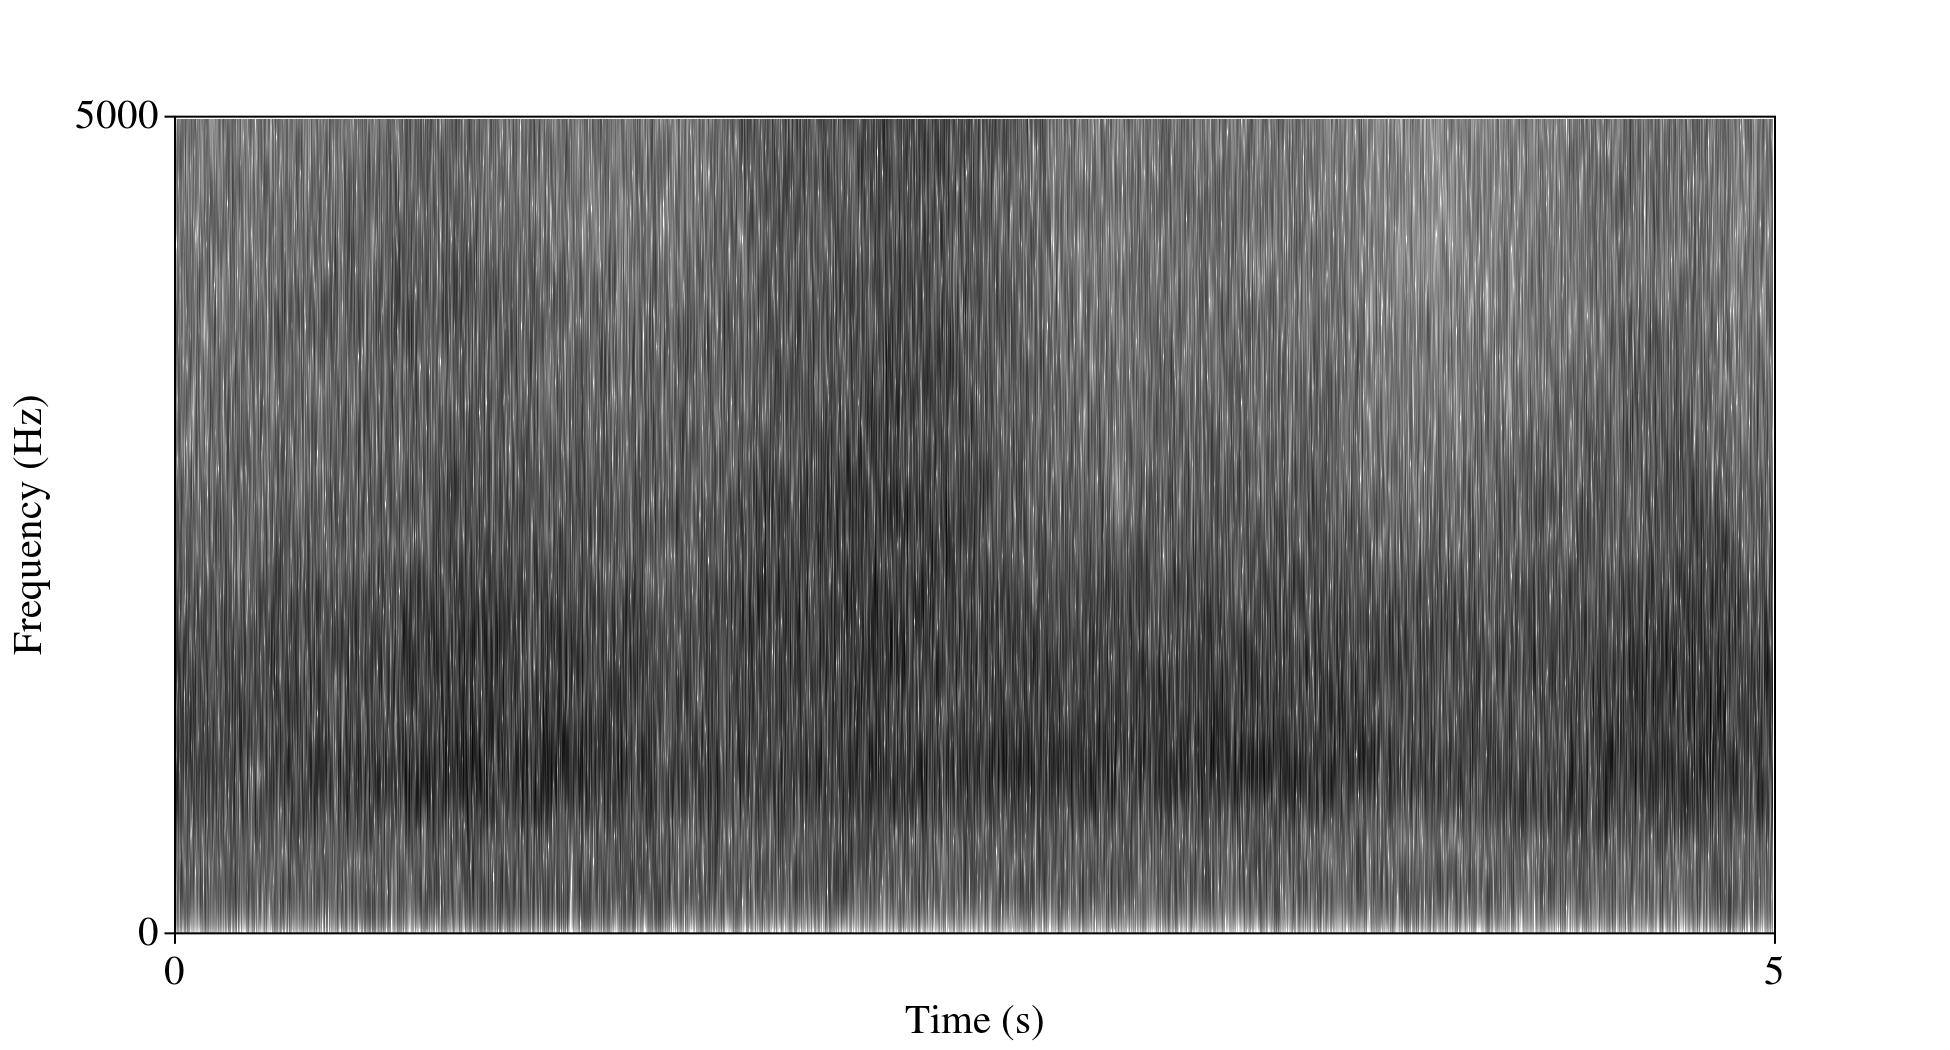
\includegraphics[width=0.9\textwidth]{figure/spctgrm-str-background.png}
  \caption{Street background noise.}
  \label{fig:str-bkgrnd}
\end{subfigure}%
%\hfill
\\[2ex]
\begin{center}
\begin{subfigure}{0.475\linewidth}
  \centering
  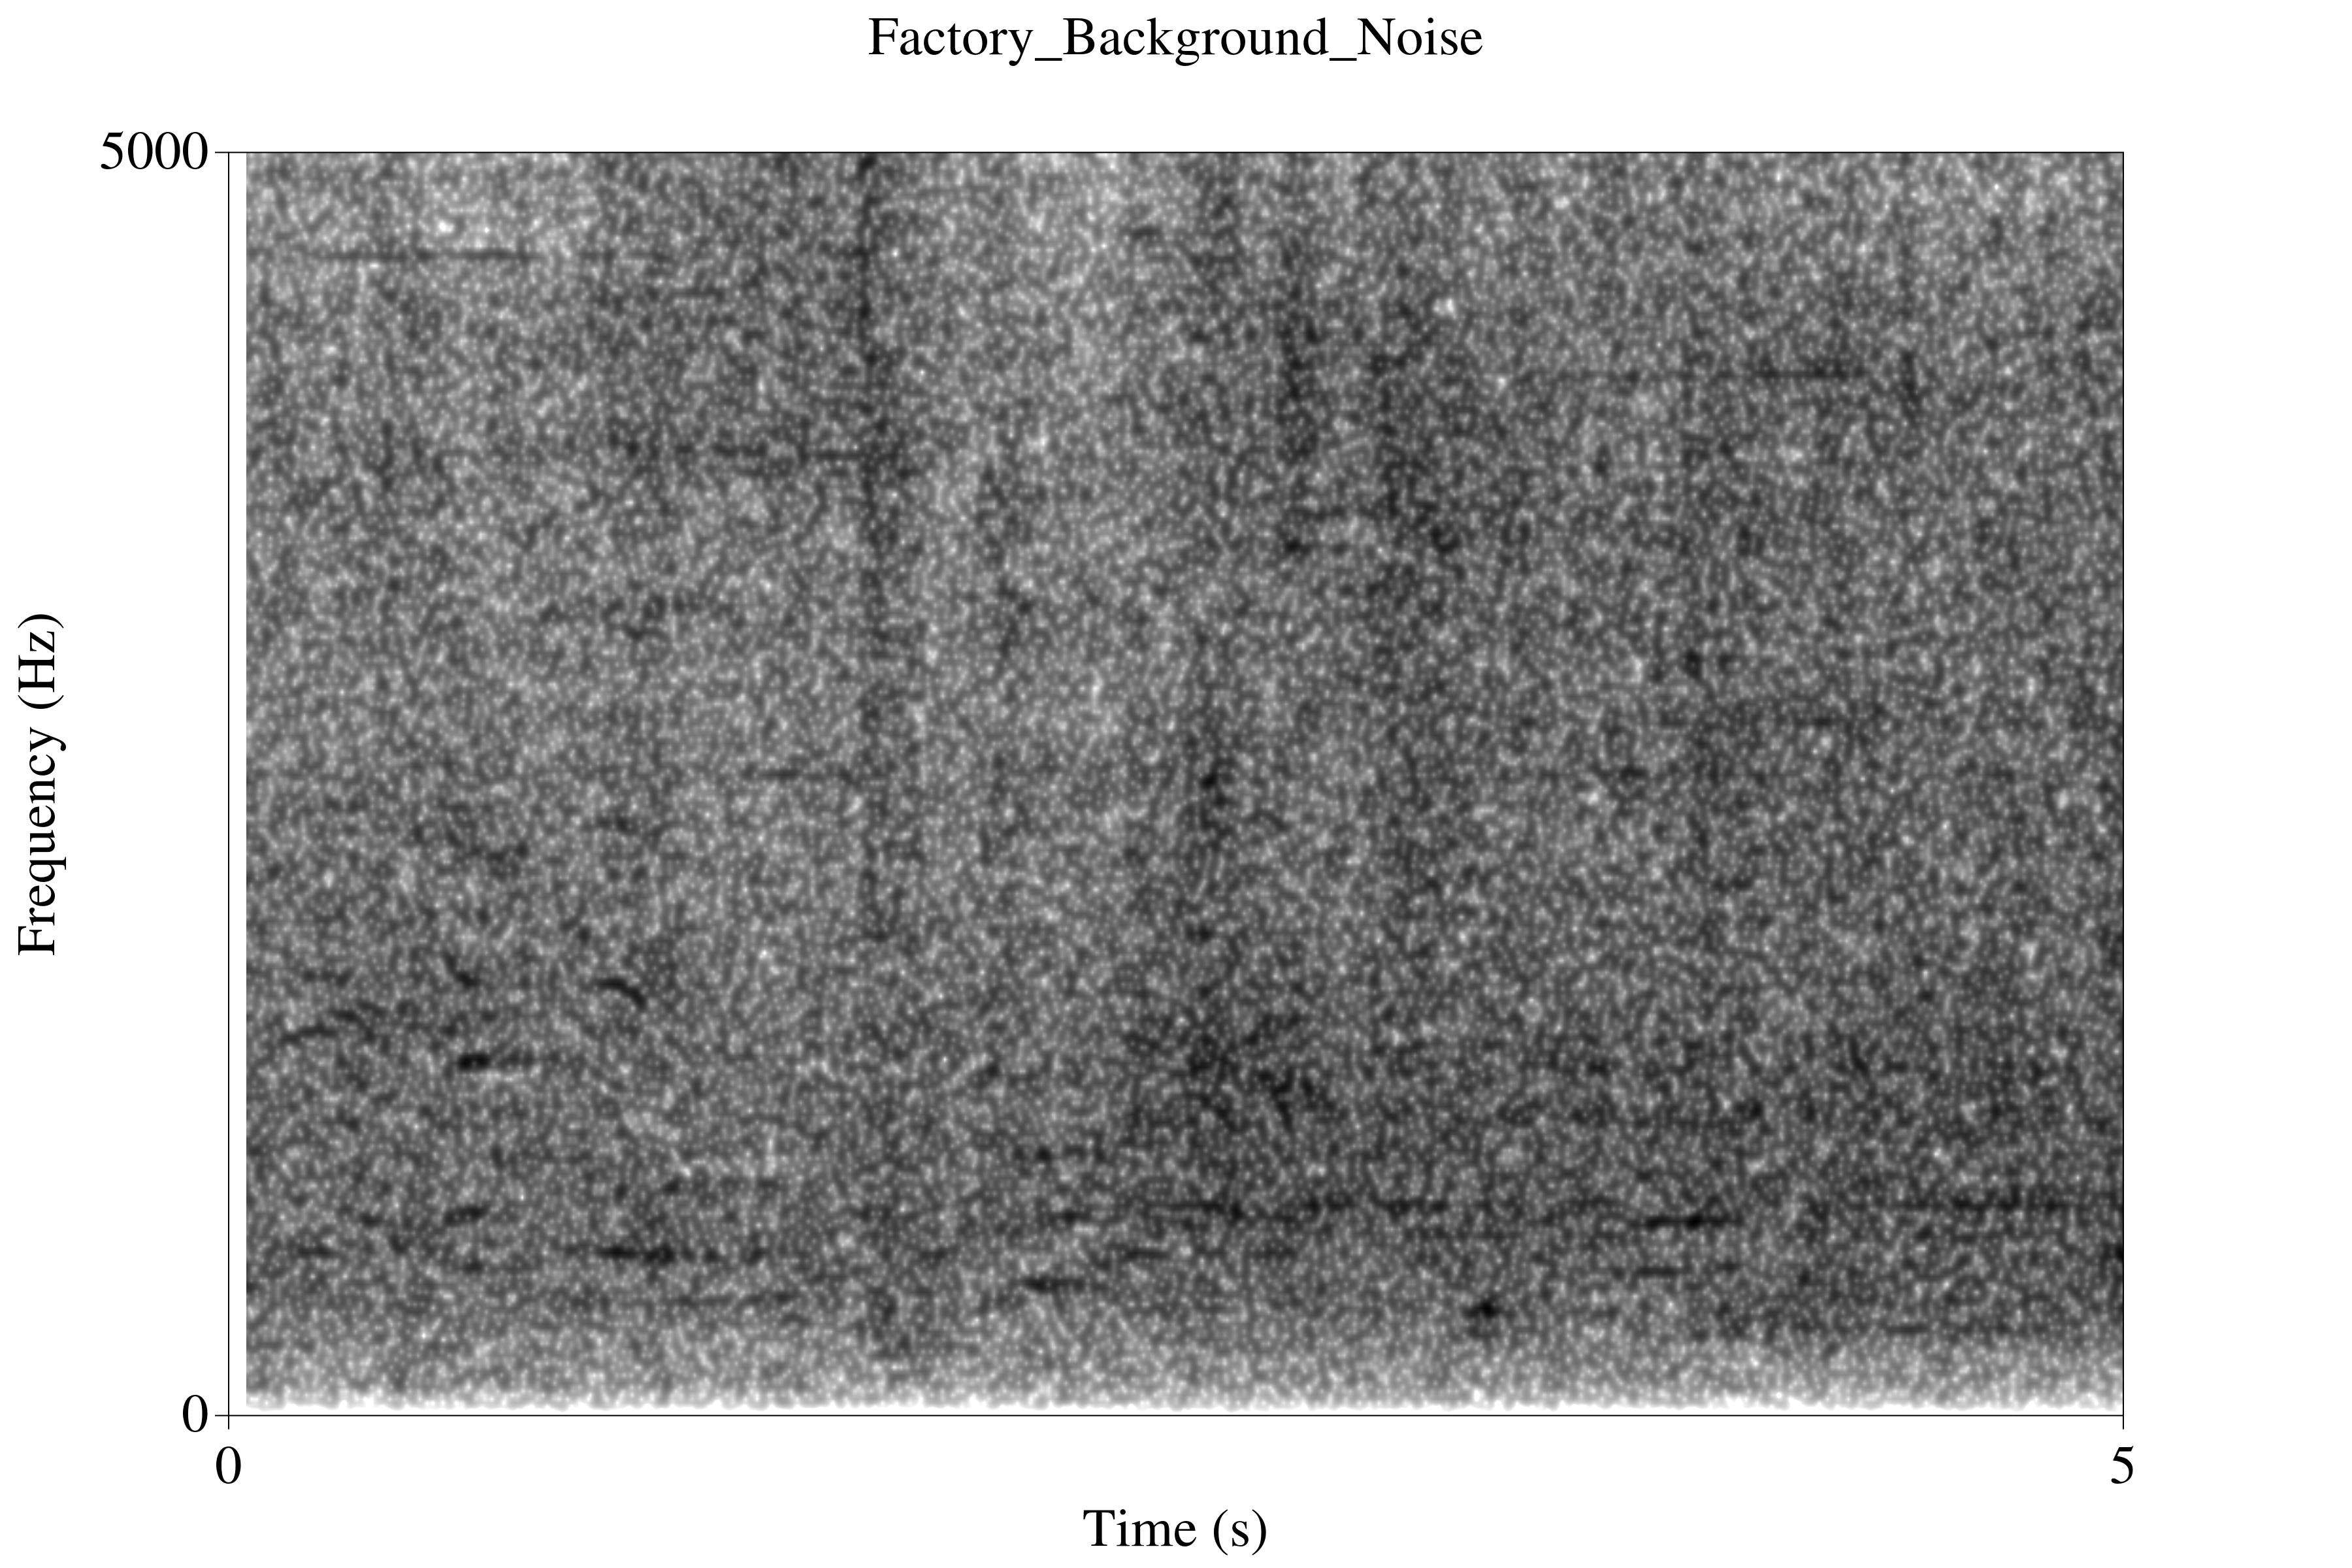
\includegraphics[width=0.9\textwidth]{figure/spctgrm-fac-background.png}
  \caption{Factory background noise.}
  \label{fig:fac-bkgrnd}
\end{subfigure}
\end{center}
\caption{Example spectograms of the first five seconds of the background noise tracks. Most recorded sentences occurred within these temporal spans.}
\label{fig:bkgrnd-noises}
\end{figure}

Yet simply because a sound may be ``masked'' does not necessarily imply that the voice is not heard or understood.  There are a number of methods used by the auditory system to overcome the masking and interpret the voice; this process is termed ``release from masking'' (\cite{middlebrooks:17}).  One such proposed method, the use of humans' built in binaural hearing, uses both ears to tease apart the different sources, utilizing the very small temporal difference that occurs when different sound sources reach each ear.  
In this example, it is easy to see that energetic and informational masking are not strictly limited to masking separate ``lower'' and ``higher'' processes (\cite{durlach:06}).
The use of binaural hearing is an example of utilizing a ``higher'' process as a release from energetic masking, as it necessarily requires signals from both ears to be interpreted (\cite{hirsh:48}). Binaural hearing is essentially making use of the spatial directionality of the noise(s) from the listener to separate the different sources (\cite{bregman:94}).

There are many other proposed methods of release from energetic masking. One involves making note of acoustic transitions: ``when [a] sound...changes its properties gradually, [it] is likely to be heard as a single changing sound.  However, when [it] changes...abruptly, [it] tends to be treated as a newly arriving sound, this tendency increasing with the abruptness of the change.'' (\cite{bregman:94}, 5).  The use of fundamental frequency (F0) has also been shown to be an effective tool, presumably to interpret the location of harmonics, and parse apart different sources (eg. two separate, simultaneous vowels with different F0s, (\cite{bird:97})). There are many other proposed methods to release masking that the auditory system uses, particularly among informational masking (\cite{middlebrooks:17}), but these are beyond the scope of this project.


\subsection{Performance of Human Recognition of Speech in Noise}

Eventually, however, with enough background noise and masking, the methods listed above for releasing the masking will fail and recognition will begin to break down.  Under the most simple conditions to measure - steady-state noise - \cite{ding:13} report that when listening to speech in noise, human self reported intelligibility ratings don't drop significantly until the SNR reaches approximately -3 dB, where intelligibility drops to about 55\%, and it doesn't hit near floor level (0\%) until -9 dB SNR.

This subjective measure is backed by a study performed by \cite{gilbert:13}, who used the PRESTO corpus (\cite{garofolo:93}) to test sentence intelligibility among 121 native English speakers.  \cite{gilbert:13} found that - similar to \cite{ding:13} - the median score (at the 50th percentile) of speech with a -3dB SNR had about 55\% accuracy.  At +3 dB SNR, the median score increased to approximately 88\% accuracy.

\cite{ding:13} do however mention that there was great inter-speaker variation among the reported subjective perception of intelligibility of an utterance; this is also supported by \cite{gilbert:13}'s results. They showed that, averaging over all SNR conditions (-5, -3, 0, +3 dB), the variability between speaker's accuracy scores had a range of almost 36\% for a given item.  A retest performed with a subgroup of the original participants on the same dataset yielded a similar (~34\%) range of variability in accuracy.  

\cite{francis:10} discusses how listening to speech in background noise places extra demands on working memory, as does listening to degraded speech (\cite{francis:09}).  The diversion of working memory to acoustic processing can be particularly detrimental to performance when simultaneously working on other computation, e.g. syntactic and semantic parsing (\cite{caplan:99}), such as in phrase or sentence recognition. \cite{tamati:13} tested a group of high-performing hearers of speech in noise against a separate group of low-performing hearers using several different working- and short-term memory tasks.  Not surprisingly, the group of listeners who are able to better hear speech in noise also perform statistically better on the working memory tasks.  Working- and short-term memory are by no means the only indicators of perceptual performance.

\cite{mattys:12} briefly discusses the concept of perceptual learning, which asserts that one can learn to accommodate a particular adverse condition (eg. background noise, signal distortion, etc.) with practice in that area.  Learning will be less effective in cases which the degradation is variable or unpredictable between trials, such as with unpredictable background noise.  The speech with the background noises in this present study will be presented in a random order, and since the background noise varies, it cannot be assumed or predicted from one sentence to the next, and therefore likely will not be `learned' in this sense.

Although there is expected to be a great amount of variability between subjects, the results from the \cite{ding:13} and \cite{gilbert:13} studies indicate that the average SNR for the highest noise condition from the data collected and described in Chapter 2\ref{chapter2}\footnote{Some of the lowest 80 dB noise condition sentences yielded approximately +6dB SNR} is over 9 dB SNR above the 50\% intelligibility threshold at -3 db SNR given by these two studies.  It is unlikely that listeners will encounter much masking in the collected noisy speech that won't be overcome.

After testing two pilot participants on the speech collected, it was deemed that the speech in the noisy background (described in Chapter 2\ref{chapter2}) was too easily recognizable.  This conclusion was drawn because the average performance on noisy speech (using word error rate (WER)\footnote{The lower the error rate, the more accurate}) was at a very low 10\% using only the 80 dB noise condition; the average non-noisy mouth-recorded speech was only slightly more accurate at 7\% word error rate. The cause was likely that the SNR ratio was not low enough, as explained in Section \ref{ch2:limitations}.  Due to this, two additional participants were rerun with lower SNRs, explained more in Section \ref{expt3}.

%Experiment redo

% Rediscuss these (learning directly above, cover briefly) in brief background when introducing secondary studies)
%PERCEPTUAL LEARNING AS IMPETUS FOR READING TRAINING TASK
%FREQUENCY as release of energetic masking AS IMPETUS FOR COMBINATION STIMULI


\section{Experiment 3: Human Speech Perception in Noise}
\label{expt3}

After additional stimuli were gathered from two additional participants (explained below in Section \ref{chap4:methods:stimuli}), a human speech perception experiment was run on the data in order to better understand and compare the ability of the auditory system to accurately comprehend the speech with a noisy background and the [modified] speech distorted by passage through the speaker's head.  To act as a control, participants would also listen to the normal, clean speech.

\subsection{Stimulus Generation}
\label{chap4:methods:stimuli}

To remedy the problem of the noisy speech being \textit{too} intelligible and having a high SNR, 
%
\begin{wrapfigure}{r}{0.5\textwidth}
\centering
  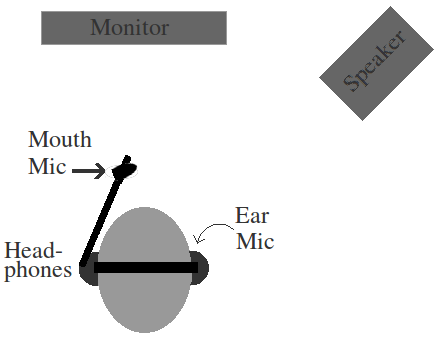
\includegraphics[width=0.45\textwidth]{figure/overallSetUp_new.png}
  \caption{This is the same setup as described in Chapter 2\ref{chapter2}, except that the mouth microphone is facing the loudspeaker, rather than the mouth.}
  \label{fig:overallSetUp_new}
\end{wrapfigure}
%
two additional participants (one male, one female) were recorded following the procedure in the first task (cf. Chapter 2\ref{chapter2}).  The list of stimuli was increased to 80 sentences (eight Harvard Sentence lists\footnote{This included the previous three lists, 14, 28, and 57, as well as lists 21, 29, 37, 53, and 68. These additional lists were pseudo-randomly chosen, as were the original three lists, to contain words that would be readily recognizable by the participant population.}) to provide more reaction data from this present experiment.  

To decrease the SNR, the directional microphone was pointed away from the mouth of the participants, and directed toward the loudspeaker (see Fig. \ref{fig:overallSetUp_new}).  This differs from the options for remedying the problem of high SNR, which were listed in Chapter 2\ref{chapter2} Section \ref{ch2:limitations}.  Options (a) - having the speaker intentionally lower their spoken volume - and (b) - increasing the background noise - were deemed unreliable and impractical.  Option (c) - using an omnidirectional microphone - was not considered for this small data collection task due to the lack of availability of omni-directional microphones that fit the size and specification requirements.

Regardless, pointing the directional microphone towards the loudspeaker still results in some of the limitations outlined in Section \textit{\textbf{[Chapter 2: Limitations]}}\ref{ch2:limitations} in Chapter 2\ref{chap2}.  It shares the same issue as the omnidirectional microphone, namely that pointing the mouth-microphone toward the loudspeaker, rather than increasing the noise, ignores the fact that the noise level inside the ear canal might increase as well with an increase in ambient noise.  Given the alternatives outlined in Section \ref{ch2:limitations}, this was seen as the best available option.  Figures \ref{fig:spectNewMouthNoise} and \ref{fig:spectNewEarNoise} show the new noisy and ear recorded speech, respectively.
%
\begin{figure}
\begin{subfigure}{0.5\textwidth}
  \centering
  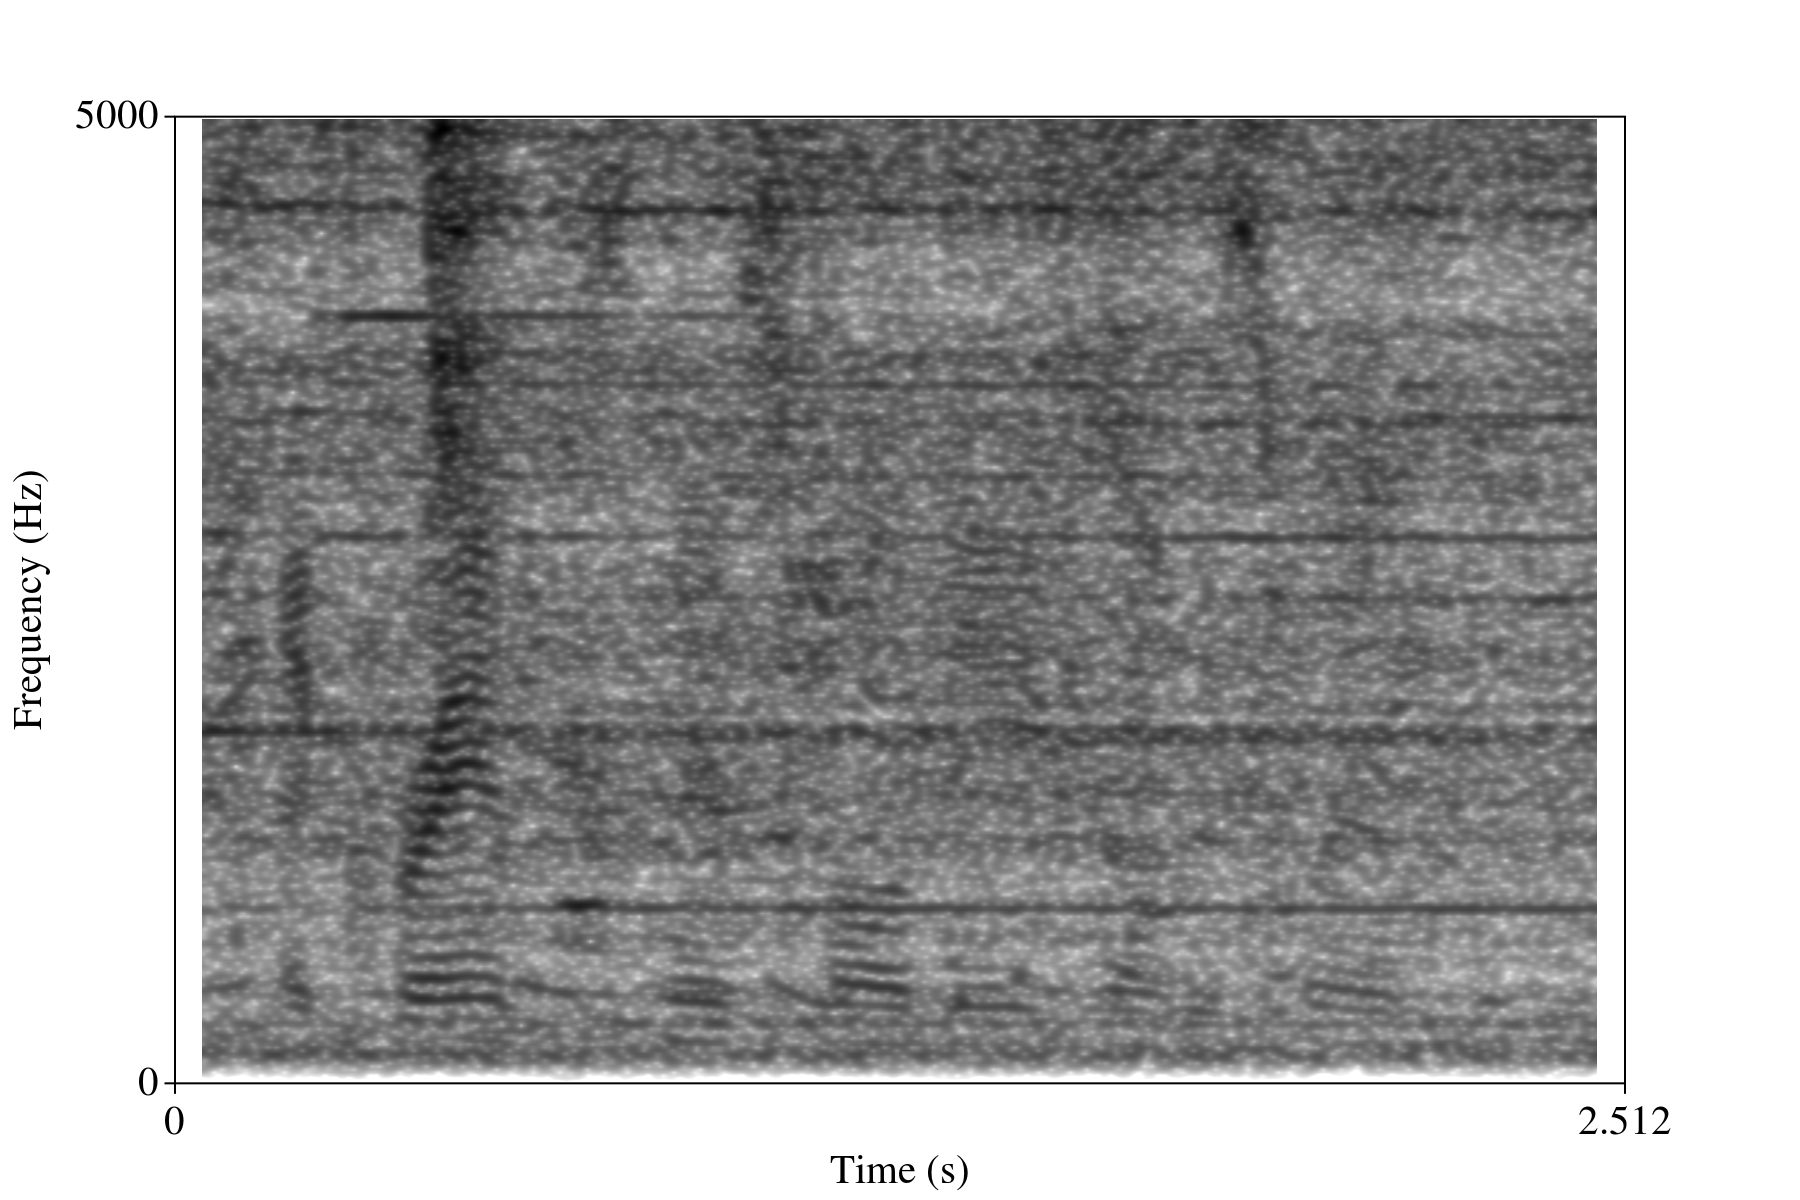
\includegraphics[width=0.9\textwidth]{figure/spectNewMouthNoise.png}
  \caption{New recording at the mouth with the microphone pointed toward the loudspeaker noise source.}
  \label{fig:spectNewMouthNoise}
\end{subfigure}
%
\begin{subfigure}{0.5\textwidth}
  \centering
  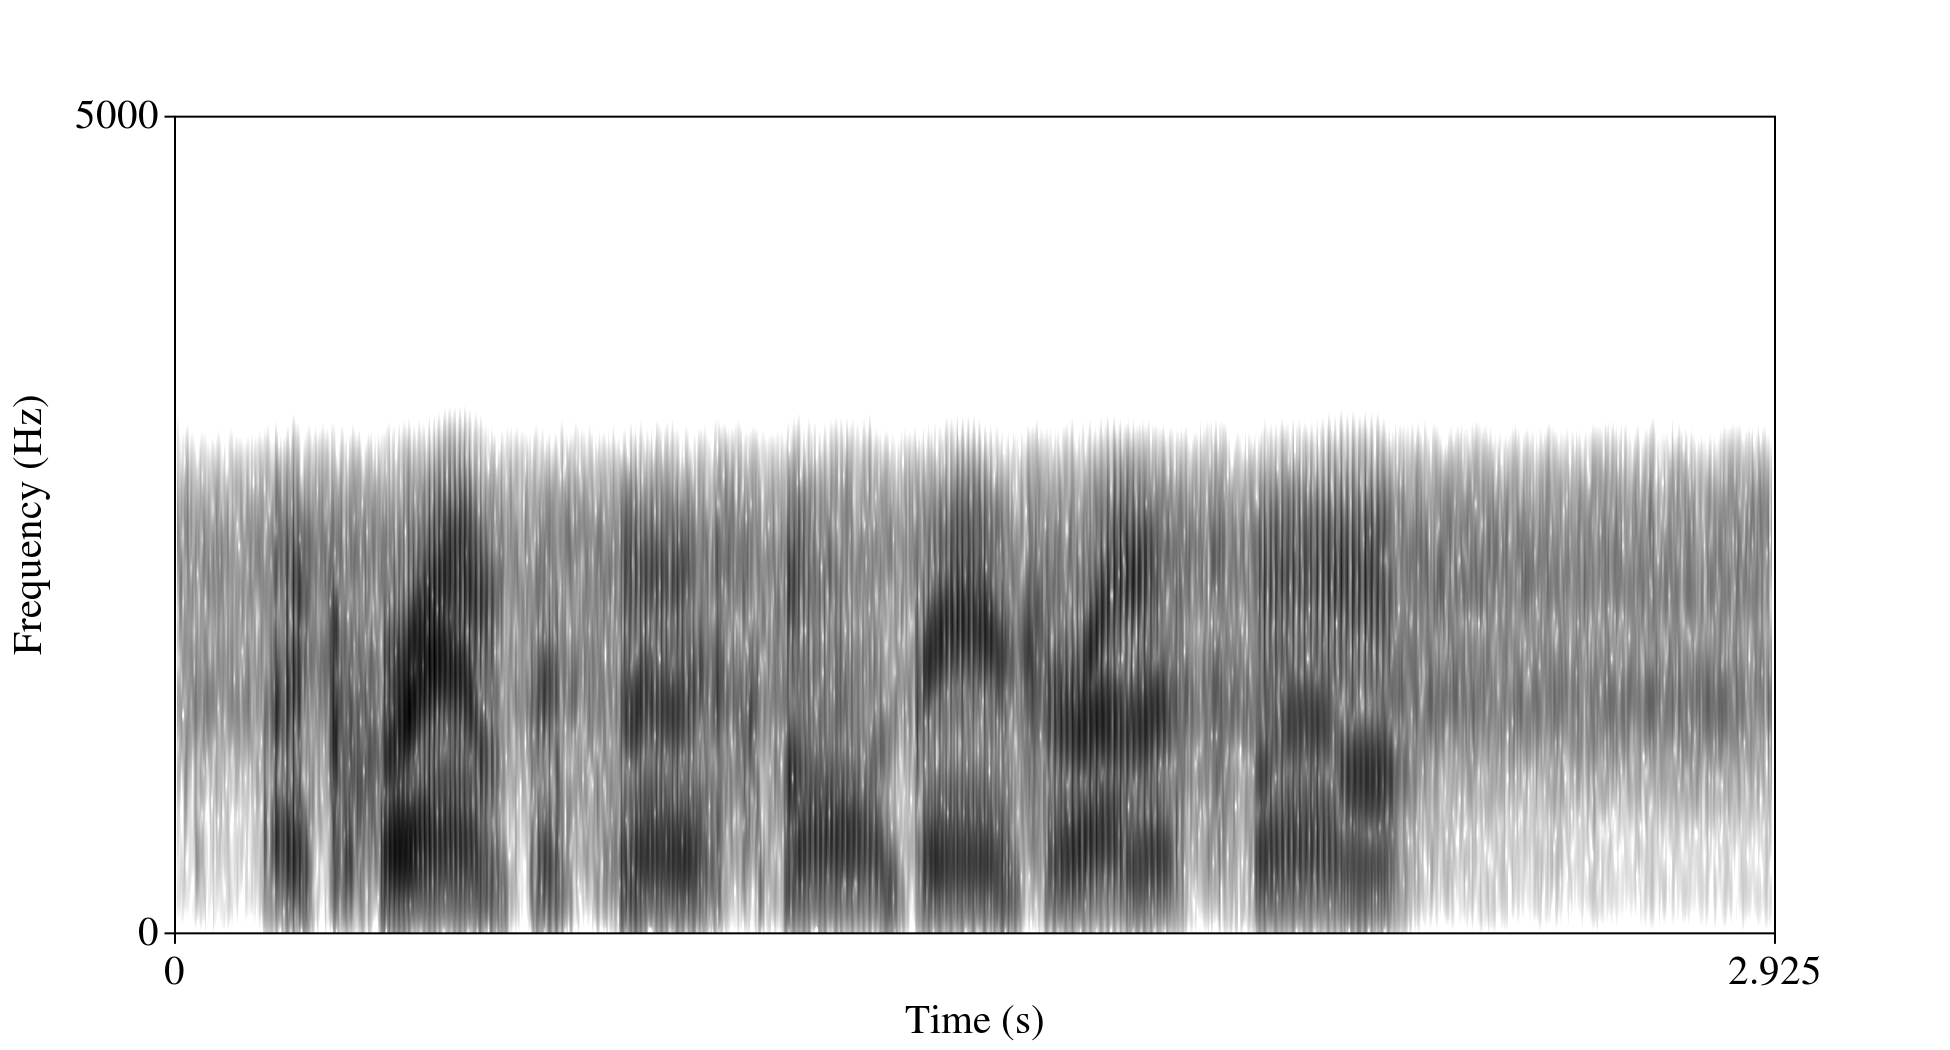
\includegraphics[width=0.9\textwidth]{figure/spectNewEarNoise.png}
  \caption{New recording at the ear; all recording conditions for the ear were the same as in the first group of recordings.}
  \label{fig:spectNewEarNoise}
\end{subfigure}
\caption{The sentence ``A cramp is no small danger on a swim'' spoken by the male speaker, recorded at the mouth (Fig. \ref{fig:spectNewMouthNoise}) with `caf\'{e} noise, and simultaneously at the ear (Fig. \ref{fig:spectNewEarNoise}).}
\end{figure}


Furthermore, due to the issue of the lack of noise in the noisy speech signals, only one noise level condition was used - the highest available noise level (80 dB).  All previously used background noise types were used for this data collection task as well.


\subsection{Design}
\label{chap4:methods:design}

The experiment had three factors - gender of speaker\footnote{This has been included to ensure there is no effect of gender on perception in noise or on transmission of speech through the head and into the ear canal, due to the difference in male and female vocal tracts.} \textbf{x} microphone location \textbf{x} noise type - resulting in a 2x2x6 experiment.  There were two genders, two mic locations (recording at the ear, and at the mouth), and six noise types (bus, caf\'{e}, pedestrian, street, factory, and no noise (clean)).  Since the ability to understand speech in noise is quite variable between individuals, the design of this experiment was a within-subjects experiment.  This meant that each of the 2x2x6 (ie. 24) conditions needed to be heard by each participant.  The sessions that were re-recorded utilized 80 distinct sentences, which allowed for three sentences to appear in each of the 24 conditions, totaling 72 sentences used in the experiment.  The eight remaining sentences were used as a ``training'' set, intended to get the participants used to the task itself, rather than to acclimate them to the type of speech that they would hear.

Since any given participant could not hear the same sentence twice without introducing a confound, and since each sentence was recorded in each of the 24 conditions\footnote{72 distinct sentences * 24 conditions = 1728 total sentence recordings}, this necessitated the use of 24 counterbalanced groups to ensure that each sentence was heard in every condition by at least one participant listener.  For example, sentences 1, 2, and 3 would occur in Condition \#1 (e.g. female speaker, mic at the mouth, with bus background noise) in counterbalanced group \#1 for Participant \#1. Participant \#2 would see counterbalanced group \#2, which placed sentences 1, 2, and 3 in Condition \#2 (e.g. female speaker, mic at the mouth, with caf\'{e} background noise).  For simplicity's sake, each grouping of three sentences would appear together in a given condition, and were not mixed up between the different counterbalanced groups.  However, once the sentences are assigned to a particular condition, the order of presentation to the participants is randomized.

\subsection{Participants}

Twenty-four native speakers of English with self-reported normal hearing participated in the experiment. Each participant was placed into a separate counterbalanced group, as specified above in Section \ref{chap4:methods:design}.

\subsection{Equipment}

The experiment was conducted in a soundbooth with a pair of over-the-ear headphones.  The experiment interface utilized in-house developed software, and participants' answers were typed into a textbox in this program, on a computer whose monitor could be seen from inside the soundbooth.

\subsection{Procedure}
\label{hsp-main-procedure}

The participant was seated in the sound booth in front of a keyboard and computer monitor with a pair of headphones, and was given a set of instructions. They were told that they would hear each utterance only once, and what they would hear was comprised of real English words, but may not constitute a ``complete'' sentence.  They were forewarned that many of the sentences they would hear would be noisy and difficult to understand. They were instructed to write all words they heard, even if what was heard did not make syntactic sense, or if the words were not adjacent (e.g. if only the first and last word of the sentence was heard). They would be timed, with 18 seconds to type their response starting from the beginning of the sound file and that their answer would be saved as-is if they ran into the time limit, preventing them from typing more.

The participant was told that the first set of eight utterances they heard were part of a ``training'' set of eight utterances intended to familiarize them with the task\footnote{The same eight sentences were heard by every participant}.  None of the utterances from the training set were used in the analysis.  Once completed with this initial set, participants were asked if they had any questions.  Afterwards they began the primary task in the soundbooth.  They would hear one of the sentences, and type their answer in a text box.  When finished with their answer, they would either click to advance to the next sentence, or, if they ran into the time limit, were prevented from modifying their answer, and were prompted to click another button to advance.  When finished with all 72 stimuli, the participant was given a brief questionnaire to fill out.  

After the experiment, the researcher would double check participant answers for correct spelling.  Only obvious errors were modified (e.g. `teh' to `the', `crakers' to `crackers', `mantle' to `mantel'), while ambiguous errors were left as-is (e.g. `blo' was not changed to `block', `finde' was not changed to `fine').  Numbers were also lexicalized (e.g. `30' to `thirty').  Punctuation was removed for ease of analysis and calculation of word error rate.  Exact responses given by each participant can be found in Appendix F\ref{appendixF}.


\section{Results}
\label{ch4:results}

\begin{knitrout}
\definecolor{shadecolor}{rgb}{0.969, 0.969, 0.969}\color{fgcolor}
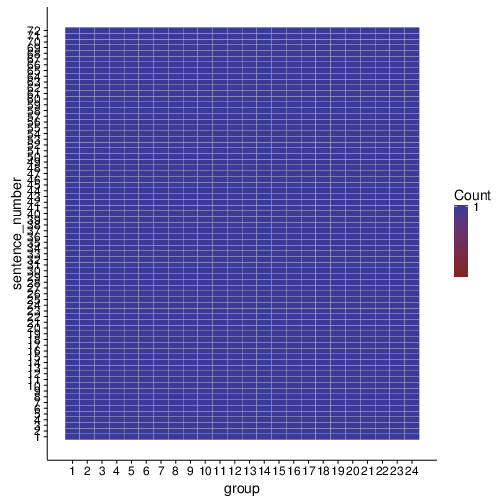
\includegraphics[width=\maxwidth]{figure/Exp_1_Data-1} 

\end{knitrout}

The word error rate (WER) for each (spell-checked) response for each participant was calculated. The code for the WER calculation can be found in Appendix F\ref{appendix?}

A 3-way, within-subjects ANOVA was performed with the collected data - 72 sentences from each of the 24 participants. Factors included the gender of the speaker (of the stimulus) with two levels - male and female - the location of the recording microphone with two levels - at the mouth and at the ear - and the background noise type with six levels - no noise, bus noise, caf\'{e} noise, pedestrian noise, street noise, and factory noise.  There was no significant 3-way interaction between speaker gender, noise type, and mic location, as can be seen in the by-subjects ANOVA (Table \ref{tab:anova1_by_subj}) and the by-items ANOVA (Table \ref{tab:anova1_by_item}). Two, two-way interactions were significant, speaker gender \textbf{x} mic location, and noise-type \textbf{x} mic location. The two way interaction between speaker gender and noise type was not significant.  The main effects of all three factors were also significant (cf. Tables \ref{tab:anova1_by_subj} and \ref{tab:anova1_by_item}).

% latex table generated in R 3.4.1 by xtable 1.8-2 package
% Sun Jul 23 18:27:04 2017
\begin{table}[ht]
\centering
\begin{tabular}{lrrrrl}
  \hline
Effect & DFn & DFd & F & p & p$<$.05 \\ 
  \hline
speaker\_gender & 1.00 & 23.00 & 6.69 & 0.02 & * \\ 
  noise\_type & 5.00 & 115.00 & 84.83 & 0.00 & * \\ 
  mic\_location & 1.00 & 23.00 & 155.07 & 0.00 & * \\ 
  speaker\_gender:noise\_type & 5.00 & 115.00 & 0.55 & 0.74 &  \\ 
  speaker\_gender:mic\_location & 1.00 & 23.00 & 18.53 & 0.00 & * \\ 
  noise\_type:mic\_location & 5.00 & 115.00 & 55.53 & 0.00 & * \\ 
  speaker\_gender:noise\_type:mic\_location & 5.00 & 115.00 & 1.61 & 0.16 &  \\ 
   \hline
\end{tabular}
\caption{ANOVA for by-subjects analysis of the three-factor, within-subjects experiment.} 
\label{tab:anova1_by_subj}
\end{table}
% latex table generated in R 3.4.1 by xtable 1.8-2 package
% Sun Jul 23 18:27:05 2017
\begin{table}[ht]
\centering
\begin{tabular}{lrrrrl}
  \hline
Effect & DFn & DFd & F & p & p$<$.05 \\ 
  \hline
speaker\_gender & 1.00 & 71.00 & 4.01 & 0.05 & * \\ 
  noise\_type & 5.00 & 355.00 & 103.50 & 0.00 & * \\ 
  mic\_location & 1.00 & 71.00 & 354.53 & 0.00 & * \\ 
  speaker\_gender:noise\_type & 5.00 & 355.00 & 0.52 & 0.76 &  \\ 
  speaker\_gender:mic\_location & 1.00 & 71.00 & 21.36 & 0.00 & * \\ 
  noise\_type:mic\_location & 5.00 & 355.00 & 71.03 & 0.00 & * \\ 
  speaker\_gender:noise\_type:mic\_location & 5.00 & 355.00 & 1.86 & 0.10 &  \\ 
   \hline
\end{tabular}
\caption{ANOVA for by-items analysis of the three-factor, within-subjects experiment.} 
\label{tab:anova1_by_item}
\end{table}



Mauchley's Test for Sphericity\footnote{Sphericity assumes that the variance between levels of a factor are the same; sphericity is violated when this is not the case.} was conducted, both for the by-subjects and by-items ANOVAs.  Significant sphericity violations were found for the main effect of noise type, and the interaction of speaker gender and noise type, as can be seen in Tables \ref{tab:anova1_subj_sph_test} and \ref{tab:anova1_item_sph_test}. 

% latex table generated in R 3.4.1 by xtable 1.8-2 package
% Sun Jul 23 18:27:05 2017
\begin{table}[ht]
\centering
\begin{tabular}{lrrl}
  \hline
Effect & W & p & p$<$.05 \\ 
  \hline
noise\_type & 0.21 & 0.00 & * \\ 
  speaker\_gender:noise\_type & 0.61 & 0.73 &  \\ 
  noise\_type:mic\_location & 0.39 & 0.13 &  \\ 
  speaker\_gender:noise\_type:mic\_location & 0.67 & 0.87 &  \\ 
   \hline
\end{tabular}
\caption{Sphericity test for the by-subjects ANOVA.} 
\label{tab:anova1_subj_sph_test}
\end{table}
% latex table generated in R 3.4.1 by xtable 1.8-2 package
% Sun Jul 23 18:27:05 2017
\begin{table}[ht]
\centering
\begin{tabular}{lrrl}
  \hline
Effect & W & p & p$<$.05 \\ 
  \hline
noise\_type & 0.78 & 0.26 &  \\ 
  speaker\_gender:noise\_type & 0.64 & 0.01 & * \\ 
  noise\_type:mic\_location & 0.85 & 0.66 &  \\ 
  speaker\_gender:noise\_type:mic\_location & 0.86 & 0.70 &  \\ 
   \hline
\end{tabular}
\caption{Sphericity test for the by-items ANOVA.} 
\label{tab:anova1_item_sph_test}
\end{table}


The corrections for sphericity were performed using a Greenhouse-Geisser test, for both by-subjects (Table \ref{tab:anova1_subj_sph_corr}) and by-items (Table \ref{tab:anova1_item_sph_corr}) ANOVAs.  Neither resulted in a change to any prior finding.

% latex table generated in R 3.4.1 by xtable 1.8-2 package
% Sun Jul 23 18:27:05 2017
\begin{table}[ht]
\centering
\begin{tabular}{lrrl}
  \hline
Effect & GGe & p[GG] & p[GG]$<$.05 \\ 
  \hline
noise\_type & 0.61 & 0.00 & * \\ 
  speaker\_gender:noise\_type & 0.86 & 0.71 &  \\ 
  noise\_type:mic\_location & 0.77 & 0.00 & * \\ 
  speaker\_gender:noise\_type:mic\_location & 0.87 & 0.17 &  \\ 
   \hline
\end{tabular}
\caption{Sphericity corrections for the by-subjects ANOVA.} 
\label{tab:anova1_subj_sph_corr}
\end{table}
% latex table generated in R 3.4.1 by xtable 1.8-2 package
% Sun Jul 23 18:27:05 2017
\begin{table}[ht]
\centering
\begin{tabular}{lrrl}
  \hline
Effect & GGe & p[GG] & p[GG]$<$.05 \\ 
  \hline
noise\_type & 0.91 & 0.00 & * \\ 
  speaker\_gender:noise\_type & 0.87 & 0.73 &  \\ 
  noise\_type:mic\_location & 0.94 & 0.00 & * \\ 
  speaker\_gender:noise\_type:mic\_location & 0.95 & 0.11 &  \\ 
   \hline
\end{tabular}
\caption{Sphericity corrections for the by-subjects ANOVA.} 
\label{tab:anova1_item_sph_corr}
\end{table}

Noting the sphericity violations involving the noise type condition, the data was viewed in the box plots in Figures \ref{fig:anova1_noise_boxplot}, \ref{fig:anova1_noiseXspkr_boxplot}, and \ref{fig:anova1_noiseXmic_boxplot}.
When viewing the simple effects of noise in Figure \ref{fig:anova1_noise_boxplot}, it is apparent (and intuitive) that the no-noise condition differs distinctly from the other noise types.

This holds true when viewing the interaction of speaker gender \textbf{x} noise type in 
%
\begin{wrapfigure}{l!}{0.5\textwidth}

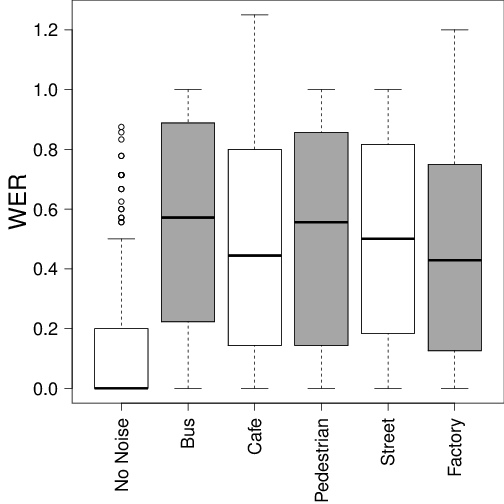
\includegraphics[width=\maxwidth]{figure/boxplot_noise-1} 

\caption{Boxplot displaying the average word error rate (WER) averaged over each participant for every noise type. WER is the variable on the y-axis, and noise type is on the x-axis.}
\label{fig:anova1_noise_boxplot}
\end{wrapfigure}
%
Figure \ref{fig:anova1_noiseXspkr_boxplot} and the interaction of noise type \textbf{x} mic location in Figure \ref{fig:anova1_noiseXmic_boxplot}.The conditions in which there is no noise present differs noticeably from those with noise; this can visually be seen even in the condition in which the speech was recorded at the ear. This is likely the root of the sphericity violations.

%\begin{wrapfigure}{L}{1\textwidth}
\begin{figure}[h!]

\includegraphics[width=\maxwidth]{figure/boxplot_noiseXspkr-1} 

\caption{Boxplot displaying the average word error rate (WER) averaged over each participant for the interaction of every noise type by the speaker gender. WER is the variable on the y-axis, and noise type by speaker gender is on the x-axis.}
\label{fig:anova1_noiseXspkr_boxplot}
\end{figure}

\begin{figure}[h!]%{L}{\textwidth}

\includegraphics[width=\maxwidth]{figure/boxplot_noiseXmic-1} 

\caption{Boxplot displaying the average word error rate (WER) averaged over each participant for the interaction of every noise type by the mic location. WER is the variable on the y-axis, and noise type by mic location is on the x-axis.}
\label{fig:anova1_noiseXmic_boxplot}
\end{figure}


Since there is a statistical difference in the main effect of noise, and since the ``no noise'' condition is very apparently different from the other noise conditions, another ANOVA was calculated with the ``no noise'' level of noise type removed.  This was to test for statistical difference only in noise conditions containing actual noise (and any resulting interaction). This modified ANOVA is a two by two by five design, with the noise type factor only having 5 levels (with the ``no noise'' condition removed from the noise type factor).

The results are similar, with no significant three-way interaction, and - as before - two significant two-way interactions of speaker gender \textbf{x} mic location and noise-type \textbf{x} mic location (cf. Tables \ref{tab:anova2_by_subj} and \ref{tab:anova2_by_item}, respectively).  There are main effects of noise type and mic location.  The main effect of speaker gender differs from the first ANOVA in that it is only significant in the by-subjects ANOVA, but is not significant in the by-items ANOVAs.

% latex table generated in R 3.4.1 by xtable 1.8-2 package
% Sun Jul 23 18:27:06 2017
\begin{table}[ht]
\centering
\begin{tabular}{lrrrrl}
  \hline
Effect & DFn & DFd & F & p & p$<$.05 \\ 
  \hline
speaker\_gender & 1.00 & 23.00 & 5.26 & 0.03 & * \\ 
  noise\_type & 4.00 & 92.00 & 5.95 & 0.00 & * \\ 
  mic\_location & 1.00 & 23.00 & 215.08 & 0.00 & * \\ 
  speaker\_gender:noise\_type & 4.00 & 92.00 & 0.60 & 0.66 &  \\ 
  speaker\_gender:mic\_location & 1.00 & 23.00 & 16.68 & 0.00 & * \\ 
  noise\_type:mic\_location & 4.00 & 92.00 & 6.00 & 0.00 & * \\ 
  speaker\_gender:noise\_type:mic\_location & 4.00 & 92.00 & 1.14 & 0.34 &  \\ 
   \hline
\end{tabular}
\caption{ANOVA for by-subjects analysis of the three-factor, within-subjects experiment. The ``no noise'' condition was removed from the noise type factor, resulting in a 2x2x5 design.} 
\label{tab:anova2_by_subj}
\end{table}
% latex table generated in R 3.4.1 by xtable 1.8-2 package
% Sun Jul 23 18:27:06 2017
\begin{table}[ht]
\centering
\begin{tabular}{lrrrrl}
  \hline
Effect & DFn & DFd & F & p & p$<$.05 \\ 
  \hline
speaker\_gender & 1.00 & 71.00 & 3.46 & 0.07 &  \\ 
  noise\_type & 4.00 & 284.00 & 6.92 & 0.00 & * \\ 
  mic\_location & 1.00 & 71.00 & 515.73 & 0.00 & * \\ 
  speaker\_gender:noise\_type & 4.00 & 284.00 & 0.55 & 0.70 &  \\ 
  speaker\_gender:mic\_location & 1.00 & 71.00 & 20.62 & 0.00 & * \\ 
  noise\_type:mic\_location & 4.00 & 284.00 & 7.14 & 0.00 & * \\ 
  speaker\_gender:noise\_type:mic\_location & 4.00 & 284.00 & 1.35 & 0.25 &  \\ 
   \hline
\end{tabular}
\caption{ANOVA for by-items analysis of the three-factor, within-subjects experiment. The ``no noise'' condition was removed from the noise type factor, resulting in a 2x2x5 design.} 
\label{tab:anova2_by_item}
\end{table}


Again, Mauchley's Test for Sphericity was conducted, resulting only in a significant sphericity violation in the by-subjects ANOVA for noise (cf. Tables \ref{tab:anova2_subj_sph_test} and \ref{tab:anova2_item_sph_test}).  This was corrected with a Greenhouse-Geisser test, which resulted, again, in no changes to the determinations of statistical significance indicated in the ANOVAs in Tables \ref{tab:anova2_by_subj} and \ref{tab:anova2_by_item}.
% latex table generated in R 3.4.1 by xtable 1.8-2 package
% Sun Jul 23 18:27:06 2017
\begin{table}[ht]
\centering
\begin{tabular}{lrrl}
  \hline
Effect & W & p & p$<$.05 \\ 
  \hline
noise\_type & 0.26 & 0.00 & * \\ 
  speaker\_gender:noise\_type & 0.76 & 0.74 &  \\ 
  noise\_type:mic\_location & 0.58 & 0.23 &  \\ 
  speaker\_gender:noise\_type:mic\_location & 0.82 & 0.89 &  \\ 
   \hline
\end{tabular}
\caption{Sphericity test for the by-subjects ANOVA with the ``no noise'' condition removed.} 
\label{tab:anova2_subj_sph_test}
\end{table}
% latex table generated in R 3.4.1 by xtable 1.8-2 package
% Sun Jul 23 18:27:06 2017
\begin{table}[ht]
\centering
\begin{tabular}{lrrl}
  \hline
Effect & W & p & p$<$.05 \\ 
  \hline
noise\_type & 0.87 & 0.36 &  \\ 
  speaker\_gender:noise\_type & 0.88 & 0.43 &  \\ 
  noise\_type:mic\_location & 0.93 & 0.86 &  \\ 
  speaker\_gender:noise\_type:mic\_location & 0.98 & 1.00 &  \\ 
   \hline
\end{tabular}
\caption{Sphericity test for the by-items ANOVA with the ``no noise'' condition removed.} 
\label{tab:anova2_item_sph_test}
\end{table}



%(cf. Tables \ref{tab:anova2_subj_sph_corr} and \ref{tab:anova2_item_sph_corr}).

% # <<ANOVA2_sphericity_corr, echo=FALSE, results='asis'>>=
% # print(xtable(by_subj_ez_anova2$`Sphericity Corrections`, label="tab:anova2_subj_sph_corr", caption="Sphericity corrections for the by-subjects ANOVA with the ``no noise'' condition removed."), include.rownames=FALSE)
% # print(xtable(by_item_ez_anova2$`Sphericity Corrections`, label="tab:anova2_item_sph_corr", caption="Sphericity corrections for the by-items ANOVA with the ``no noise'' condition removed."), include.rownames=FALSE)
% # @




\section{Discussion}

% Points to hit here:
% X- Ear speech is more easily recognized than noisy speech from the mouth (print bar graph of mic loc simple effects)
% X- There is still a main effect of noise even when 'no noise' is removed, print bar graph w/ no 'no noise' and discuss simple effects
% X- Touch on 'near-significance' of speaker gender, how it isn't as near significant as it appears - likely an SNR effect (print graph).
% - Discuss noiseXmic interation data, re-print graph
% X-- Mention differences in mouth noise performance which come out in this interaction, medians ranging from approximately 60% (factory) to near 90% (bus); reference noise spectograms, give possible explanation
% X-- Non-noisy mouth speech is still the most easily recognized - median of zero - but non-noisy ear-speech does well for itself with a median nearing 15% WER.
% X-- There still appears to be a noticeable difference between ear-no noise and ear-noisy speech (some noise must get through), but no noticeable difference between noises within ear-speech category; nevertheless, median noisy ear-speech recognition appears to hover near 30% WER.
% X-- Comment on how this is evidence for ''predictable'' noise that is (more or less) non-varying between noise types.
% X- Look at longitudinal effects
% -- Surveys - add in later
% X- Move on to limitations
% -- Mention not all sound files had normalized amplitude - some were quite louder than others, which may be an explanation for some of the observed variability.
% -- Mention the computer screen distraction.


The primary hypotheses from Chapter 2\ref{chapter2} included (a) that the signal recorded from the ear, pre-emphasized, filtered, and pre-emphasized again, would be intelligible by human listeners, and (b) that it would be more intelligible than speech with a noisy background.  The results in Section \ref{ch4:results} above show a statistical difference between the WERs of the sentence transcriptions of the speech recorded from the ear canal and the speech recorded in front of the mouth.  This can be seen more clearly in the graph of the simple effects of microphone location, in Figure \ref{fig:mic_loc_simple}.  The speech recorded at the ear has a significantly lower transcription word error rate than the speech recorded at the mouth, collapsing over all noise conditions (this holds with or without clean speech). These primary hypotheses seem to have been validated.

A statistical interaction of speaker gender \textbf{x} mic location is found.  
Looking at a boxplot of this interaction in Figure \ref{fig:spkr-genXmic-loc}, it is apparent that the two genders have different effects on microphone location.  Based on this plot, it would appear that the female's ear-recorded speech offers less intelligibility benefit over the speech recorded at the mouth, while the male voice has more of a benefit.  This interaction seems to exist primarily because listeners are able to more accurately recognize the speech in noise when spoken by the female, rather than the male.
%
\begin{wrapfigure}{R}{0.5\textwidth}

\includegraphics[width=\maxwidth]{figure/Mic-location_simple-1} 

\caption{Simple effects of Microphone Location.}
\label{fig:mic_loc_simple}
\end{wrapfigure}
%
However, while it is possible that gender itself is causing this effect, it should also noted that - in the instance of these two particular speakers - gender is confounded with level SNR.  The average female speaker's SNR in the speech recorded at mouth in noisy conditions was higher than the male speaker's SNR\footnote{\textbf{The only noise condition was 80 dB; the male speaker averaged less than +1 dB SNR and the female speaker averaged over +8 dB SNR, using the SNR calculator described in Section \textit{[Chapter 2: Ear Recorded Speech: Discussion]}\ref{chap2:discussion} and found in Appendix E\ref{appendixE}}}.


This likely contributed to the observed statistical difference.  If the SNR is high (as it was for the female's speech), the human auditory system can utilize the methods it has to ``release the masking'' in an effective manner.  Listeners therefore perform better on speech with richer frequency information (even if there is a bit of noise), than more distorted, ``muffled'' speech.  When the reverse is true and the speech in noise has a lower SNR (as it was in the male's speech), it cannot as easily be ``released from the masking'' by the auditory system.  Thus, speech that is slightly distorted - but has clearer harmonic and formant information - can be more easily understood.  The likelihood of the statistical difference seen being caused by SNR level also makes sense, as the major difference observed in Figure \ref{fig:spkr-genXmic-loc} occurs between the two genders' speech that is recorded at the mouth (in noisy conditions).  Unfortunately, this is only speculation, as with the given data, gender is confounded with SNR.

There is also a main effect of noise.  It is obvious that the speech recorded with no background noise (particularly at the mouth) would be easier to transcribe and recognize than the speech recorded with background noise.  However, when the level of `no noise' within the noise-type factor is removed, the statistical difference within this condition remains.

A closer look at the main effect of noise-type, excluding the level of `no noise', can be seen in Figure \ref{fig:noise-type_non-no-noise_main}.

The difference here is not nearly as stark as that seen within the microphone location distinction in Figure \ref{fig:mic_loc_simple}.  Even still, there is a observable difference, particularly between the bus background noise (with the highest relative WER) and the factory background noise (with the lowest relative WER).

Referring back to Figure \ref{fig:bkgrnd-noises}, containing the spectograms of the background noises in Section \ref{bkgrnd:speech_in_noise}, it appears that the bus noise (cf. Figure \ref{fig:fac-bkgrnd}) contains bands in the frequency spectrum that contain higher amplitude.
This may adversely affect a person's ability to parse the harmonics and/or formants from the desired speech. 

Again referring to Figure \ref{fig:bkgrnd-noises}, it is unclear, however, why the caf\'{e} background noise, among the other noises, has a relatively lower WER, since it also contains many more prominent bands of frequency from speaker babble. 
Similarly, it is difficult to observe much difference between the factory background noise and the pedestrian background noise, despite the pedestrian noise having a higher upper bound.

To see if any more apparent differences can be found, Figure \ref{fig:noiseXmic2} shows the noise type factor split between the two levels of mic location, displaying what was originally seen above in Figure \ref{fig:anova1_noiseXmic_boxplot}.  
%
\begin{wrapfigure}{l}{0.5\textwidth}

\includegraphics[width=\maxwidth]{figure/spkr-gender_mic-location_interaction-1} 

\caption{Interaction between speaker gender and microphone location.}
\label{fig:spkr-genXmic-loc}
\end{wrapfigure}
%
When only looking at the noise as it occurs in the mouth-recorded condition, the differences between the levels of noise become much more stark.  In particular, the difference between the bus noise (high WER) and factory noise (relatively lower WER) greatly expands. 

This distinction reaches as low as a median of approximately 60\% WER for the factory background noise conditions, and a median of nearly 90\% WER for the bus background noise.  The variance within noise conditions also differs, with the bus noise containing less variance (upper quartile 100\% WER, lower quartile ~68\% WER) than the factory noise condition (upper quartile ~90\% WER, lower quartile ~30\% WER).  The remaining noise conditions are more similar to one another, and fall in between the two, with median WERs hovering near 80\%.  The bus noise, as seen in Figure \ref{fig:bckgrnd-noises}, seems to contain very prominent frequency bands within the frequency range that is important for speech; it is possible that this plays a role in its noticeably higher WER.

The differences between the transcription WERs of the caf\'{e}, pedestrian, and street noises have expanded slightly, but still hover fairly close together in between the bus and factory performances. No explanation is proposed for the reason for these apparent divergences.

Out of all condition combinations in Figure \ref{fig:noiseXmic2}, the WER-front-runner is quite clearly the speech recorded at the mouth with no background noise.  There was never any doubt that this would be the case, as speech with relatively little background noise is the sort of speech from which learners acquire their language model, and whereby most communication occurs.  The median WER is, unsurprisingly, 0\%, though there is some variance from perfect perception; some errors do occasionally occur. 
%
\begin{wrapfigure}{l}{0.5\textwidth}

\includegraphics[width=\maxwidth]{figure/Noise-type_simple-1} 

\caption{Simple effects of Noise Type, excluding the level of `no noise'.}
\label{fig:noise-type_non-no-noise_main}
\end{wrapfigure}
%
The ear-recorded speech in a clean environment manages to also achieve a respectable transcription WER median of approximately 15\%, with a lower quartile boundary at 0\% WER and an upper quartile boundary of 35\% WER.

Despite being more similar than their mouth recorded counterparts, there is still a noticeable difference between the ear recorded speech with no noise, and ear recorded speech in noisy conditions.  Most noise conditions recorded from the ear achieve a lower quartile boundary near 0\%, but the upper quartile boundary for most nears 60\% WER.  The median WER for noise conditions generally falls at or slightly below 30\%. 

Even though there is a higher WER than the ear-recorded no-noise condition, the ear-recorded speech in noise is quite consistent across noise categories.  This is very different from the mouth-recorded speech in noise, which vary considerably between noise conditions.  This indicates that while a noise presence hampers transcription ability and increases WER in ear-recorded conditions, the varying qualities of the different background noises were dampened to the point of having a starkly lesser effect than that which occurs in the mouth-recorded speech.

Since the ability to recognize ear-recorded speech, even in noise, is quite consistent, the conditions are right for the auditory system to `perceptually learn' the distorted ear-recorded speech, as discussed in Section \ref{chap2:background} and by \cite{mattys:12}, among others.  This, in theory, would increase the learners' recognition of the ear-recorded speech with additional exposure, further increasing the WER improvement seen with ear-recorded speech.


\begin{figure}[h!]

\includegraphics[width=\maxwidth]{figure/boxplot_noiseXmic2-1} 

\caption{Boxplot displaying the average word error rate (WER) averaged over each participant for the interaction of every noise type by the mic location. WER is the variable on the y-axis, and noise type by mic location is on the x-axis.}
\label{fig:noiseXmic2}
\end{figure}

To visualize whether the performance of participants generally improves over time, scatterplots graph participant's chronological performance with mouth-recorded and ear-recorded speech over the course of the experiment in Figures \ref{fig:linear_performance_m} and \ref{fig:linear_performance_e}. 
%
\begin{figure}[t]%{L}{0.5\textwidth}
\begin{subfigure}{0.47\textwidth}

\includegraphics[width=\maxwidth]{figure/line_graph_chrono_m-1} 

\caption{Scatterplot of all participants' WER values for responses to speech recorded at the mouth \textbf{and} in noise.}
\label{fig:linear_performance_m}
\end{subfigure}
%\hfill
\begin{subfigure}{0.47\textwidth}%{L}{0.5\textwidth}

\includegraphics[width=\maxwidth]{figure/line_graph_chrono-1} 

\caption{Scatterplot of all participants' WER values for responses to speech recorded at the ear.}
\label{fig:linear_performance_e}
\end{subfigure}
\caption{The x-axis is the order of the responses; eg. ``1'' on the x-axis is the first response given by the participants.  The x-axis only corresponds to order of response, and does not indicate the specific noise type or gender of the speaker.  A line was fitted to the data using linear regression.}
\end{figure}
%
Linear regression models were fit onto the mouth-recorded data (slope=$-0.0048728$, $R^2$=$0.0175763$, $p<0.001$), and the ear-recorded data (slope=$-0.0016076$, $R^2$=$0.003146$, $p>0.05$). 

It is important to note the linear scales both axes, particularly the y-axis, as an explanation for why the slope values themselves are so small (ie. the y-axis range is from \textit{0.0} to \textit{1.2}).  The primary take away from both graphs and both fitted regression models in Figures \ref{fig:linear_performance_m} and \ref{fig:linear_performance_e} is that participants' recognition ability seems to improve statistically over the course of the experiment for mouth-recorded (noisy) speech, but not ear-recorded speech.  It could be possible that there are statistical gains by the noisy speech simply due to greater room for improvement, but it could also be due to the presence of high frequency speech information in the signal. The speech beneath the noise is ``normal'', containing full frequency information that the participant would be used to listening for, and if participants are able to use perceptual learning to take release the noise mask, this improvement over time is the expected effect.  However, as already seen, the overall performance on noisy, mouth recorded speech still falls well below that of ear-recorded speech, even at the end of the experiment.

%Of particular interest for the goals of this study, is the fact that - although very modest - there is improvement in recognition of ear-recorded speech that appears to correlate with an increase in exposure time to the ear-recorded speech.  That is, as more ear-recorded speech is heard, participants see modest gains in their ability to correctly recognize and transcribe it.  
One potential reason that there may not have been a statistical perceptual learning effect for ear-recorded speech over the course of the experiment is that the participant was not given feedback or the correct answer.  It has been shown (\cite{davis:05}) that such feedback can improve and speed up the perceptual learning process when listeners are able to correctly identify what was said.  This will be discussed further in Section \ref{ch4:follow-up-expts} below, and a follow up investigation will be conducted pertaining to this.


\subsection{Follow-up Investigations}
\label{ch4:follow-up-expts}

To expound on the previous study, two additional investigations were performed to give insights into possible future research directions.  The impetus for the first investigation was \cite{bird:97}, which demonstrated that fundamental frequency (F0) is a tool used by the auditory system to separate a desired source from masking noise.  This follow up proposes to recombine the very clear, lower frequencies from the ear-recorded speech with the ``noisy'' upper frequencies recorded at the mouth.  

The hypothesis is that the auditory system will use the clear fundamental frequency harmonic information in the lower frequencies to extract the upper harmonics out of the noise.  Accuracy is predicted to improve over that of the low-pass filtered, ``muffled'', ear speech (which many participants subjectively observed to be annoying and difficult to understand), as more high frequency information will be present and available for listeners' auditory systems.  This speech will sacrifice the advantage of being completely or nearly ``noise-free'', to sound more natural.  Additionally, since the ear-recorded speech consists of very clean harmonics, it is hypothesized that this speech, combined with the higher frequency mouth recorded speech in the noise-free condition, will perform equal to its mouth-recorded counterpart in the noise-free condition. This will be referred to as the ``F0'' investigation.

The second investigation was based on the concept of ``perceptual learning'' discussed earlier.  This presumes that the auditory system can learn to adapt to understand speech in a degraded signal better over time.  According to \cite{mattys:12}, significant learning can occur with even a small number of training trials.  \cite{davis:05} demonstrate that during training, successful recognition of a degraded signal will help one recognize a similar signal more than unsuccessful recognition of a degraded signal.  

Based on the implications of these findings, a short story was read and was recorded from inside the ear canal for the participants in this follow up study to listen to prior to completing the experiment itself.  This will serve as a brief ``training'' for participants in preparation for the actual task. Since the type of distortion from the ear-recorded signal is regular and predictable, it is hypothesized that perceptual learning will take place, and those who have listened to the training story will perform better on ear-recorded speech than those who had not (ie. those in the primary study). This will be referred to as the ``perceptual learning'' or ``training'' investigation.


\subsection{``F0'' Investigation Methods}
\label{F0-methods}

The stimuli used for this investigation consisted of the exact same sentences produced by the exact same speakers.  No modification was performed to the sentences recorded at the mouth.  For the sentences recorded at the ear, the same modifications as before (pre-emphasis, lowpass filtering\footnote{Lowpass filtered allowing 0-2500Hz, with a 500 Hz slope}, and a second pre-emphasis) were performed, but afterwards, the simultaneously recorded speech from the mouth was filtered and combined with the ear-recorded speech.  The speech from the mouth was bandpass filtered between 3000Hz and 8000Hz, with a 500Hz slope.  
%
\begin{wrapfigure}{r}{0.5\textwidth}
\centering
  \includegraphics[width=0.45\textwidth]{figure/combined-signal.png}
  \caption{A spectrogram of the sentence ``A cramp is no small danger on a swim''.  The low-pass filtered ear-recorded signal was combined with the simultaneous [noisy] mouth signal, which was bandpass filtered at a higher frequency.}
  \label{fig:combined-signal}
\end{wrapfigure}
%
This allowed for an overlap of the frequencies from the mouth-recorded speech and the lowpass filtered ear-recorded speech.  The two signals were converted to a stereo signal, and then combined into a mono signal.  This resulted in relatively clean speech below approximately 2.7 kHz, and noisy speech above approximately 2.7 kHz, as seen in Figure \ref{fig:combined-signal}.

There were five native speakers of English with self-reported normal hearing who participated in this investigation.  The design and procedure of this task was exactly the same as the initial perception experiment, save the alteration in modifications performed on the ear-recorded stimuli, described above.


\subsection{``F0'' Results and Discussion}
\label{ch4:F0_discussion}

%\begin{wrapfigure}{L}{0.75\textwidth}

% \caption{Using the data from the five participants who performed the experiment using the speech in which the higher frequencies were added back in from the noisy mouth-recorded speech.  Boxplot displaying the average word error rate (WER) averaged over each participant for every noise type. WER is the variable on the y-axis, and noise type is on the x-axis.}
% \label{fig:F0_noise_boxplot}
% \end{wrapfigure}

% \begin{figure}%{L}{\textwidth}
% <<F0_boxplot_noiseXspkr, echo=FALSE, results='asis'>>=
% boxplot(wer~noise_type*speaker_gender,col=c("white","lightgray"),F0data, names=c("Female\nNo Noise","Female\nBus","Female\nCafe","Female\nPedestrian","Female\nStreet","Female\nFactory","Male\nNo Noise","Male\nBus","Male\nCafe","Male\nPedestrian","Male\nStreet","Male\nFactory"),ylab="WER",las=2)
% @
% \caption{Using the data from the five participants who performed the experiment using the speech in which the higher frequencies were added back in from the noisy mouth-recorded speech.  Boxplot displaying the average word error rate (WER) averaged over each participant for the interaction of every noise type by the speaker gender. WER is the variable on the y-axis, and noise type by speaker gender is on the x-axis.}
% \label{fig:F0_noiseXspkr_boxplot}
% \end{figure}

\begin{figure}[h!]%{L}{\textwidth}

\includegraphics[width=\maxwidth]{figure/F0_boxplot_noiseXmic-1} 

\caption{Using the data from the five participants who performed the task using the speech in which the higher frequencies were added back in from the noisy mouth-recorded speech.  Boxplot displaying the average word error rate (WER) averaged over each participant for the interaction of every noise type by the mic location. WER is the variable on the y-axis, and noise type by mic location is on the x-axis.}
\label{fig:F0_noiseXmic_boxplot}
\end{figure}

Since there were only five participants in this follow-up investigation, no actual statistics were run to test for significance.  The results here are to be used in a basic comparison of possible directions these altered methods may be able to take future research.

The boxplot in Figure \ref{fig:F0_noiseXmic_boxplot} demonstrates the interaction of most interest, that of noise-type and microphone location, as identified by the ANOVAs performed on the primary experiment above.  No change was made to any of the presented mouth-recorded speech signals, so, as is observed, one would not expect there to be any change to listeners' ability to recognize these signals (outside of expected inter-speaker variation).

It is interesting to note that the primary difference between the clean ear-recorded speech and the ``noisy'' ear-recorded speech appears to be the extent of the variation in the upper quartile and whiskers.  Based on what is seen here, if this follow up study were to be extended carried out in a full study, one would expect there to be a dramatic difference between the noisy speech recorded at the mouth, and the speech recorded at the ear.
Further discussion concerning the comparison of these results with those of the primary study and the ``perceptual learning'' study can be found below in Section \ref{ch4:glob_discussion}.
% %
% \begin{wrapfigure}{L}{0.5\textwidth}
% <<F0spkr-gender_mic-location_interaction, echo=FALSE, results='asis'>>=
% boxplot(wer~speaker_gender*mic_location,col=c("white","lightgray"),F0data, names=c("Female\nEar-Recorded","Female\nMouth-Recorded","Male\nEar-Recorded","Male\nMouth-Recorded"),ylab="WER")
% @
% \caption{Interaction between speaker gender and microphone location.}
% \label{fig:F0_spkr-genXmic-loc}
% \end{wrapfigure}
% %


\subsection{``Perceptual Learning'' Methods}

For this investigation, a new speaker was recorded from the ear canal (with the same set-up as all previous recordings) reciting the short story ``Peter Rabbit'', by Beatrix Potter.  The recorded story, as was presented to the participants, had a total length of approximately 5 minutes and 13 seconds.  The recorded story underwent the same transformations as the ear-recorded stimuli in the primary study (ie. pre-emphasis, lowpass filtering\footnote{Lowpass filter of 0-2500Hz with a 500Hz slope.}, and pre-emphasis again).

There were four native speakers of English with self-reported normal hearing who participated in this follow up investigation.  They were first presented with a transcript of the story, and asked to listen to the audio and read along.  This offers ample chance for ``successful'' recognition of the degraded ear-recorded signal (cf. \cite{davis:05}).  After the reading session, the participants conducted the task as was done in the other tasks mentioned in Sections \ref{hsp-main-procedure} and \ref{F0-methods}, with the exact same stimuli as in the primary experiment.

\subsection{``Perceptual Learning'' Results and Discussion}

%\begin{wrapfigure}{L}{0.75\textwidth}

% \caption{Using the data from the four participants who performed the training task in which they listened and read along to a story prior to the experiment.  Boxplot displaying the average word error rate (WER) averaged over each participant for every noise type. WER is the variable on the y-axis, and noise type is on the x-axis.}
% \label{fig:perc_noise_boxplot}
% \end{wrapfigure}

% \begin{wrapfigure}{L}{\textwidth}
% <<perc_boxplot_noiseXspkr, echo=FALSE, results='asis'>>=
% boxplot(wer~noise_type*speaker_gender,col=c("white","lightgray"),perc_data, names=c("Female\nNo Noise","Female\nBus","Female\nCafe","Female\nPedestrian","Female\nStreet","Female\nFactory","Male\nNo Noise","Male\nBus","Male\nCafe","Male\nPedestrian","Male\nStreet","Male\nFactory"),ylab="WER",las=2)
% @
% \caption{Using the data from the four participants who performed the training task in which they listened and read along to a story prior to the experiment.  Boxplot displaying the average word error rate (WER) averaged over each participant for the interaction of every noise type by the speaker gender. WER is the variable on the y-axis, and noise type by speaker gender is on the x-axis.}
% \label{fig:perc_noiseXspkr_boxplot}
% \end{wrapfigure}

\begin{figure}[h!]

\includegraphics[width=\maxwidth]{figure/perc_boxplot_noiseXmic-1} 

\caption{Using the data from the four participants who performed the training task in which they listened and read along to a story prior to the experiment. Boxplot displaying the average word error rate (WER) averaged over each participant for the interaction of every noise type by the mic location. WER is the variable on the y-axis, and noise type by mic location is on the x-axis.}
\label{fig:perc_noiseXmic_boxplot}
\end{figure}

As stated in the discussion of the ``F0'' investigation in Section \ref{ch4:F0_discussion}, there are too few participants to run actual statistics on the results of this follow up investigation, and so implications here should be taken lightly and used to prepare further future research in this area. The only difference between this investigation and the primary study are that the participants in this task heard a 5 minute, 13 second ``training'' story beforehand, recorded from the story narrator's ear.

The boxplot in Figure \ref{fig:perc_noiseXmic_boxplot} displays the interaction of noise type and microphone location, which was a statistical interaction in the primary experiment.  It can be seen that the relationship between ear- and noisy mouth-recorded speech appear to remain the same; as expected the ear-recorded speech continues to be more easily recognized than speech recorded at the mouth in noise.  Further discussion continues below.



\subsection{Discussion of All Investigations}
\label{ch4:glob_discussion}

Looking into the differences between the primary study and the two follow-up studies, Figure \ref{fig:ALLXperc_noiseXmic_mouth_boxplot} shows the difference between the mouth-recorded speech in each of these three studies.  Given that no change was actually made to the audio of the mouth-recorded speech between these different experiments, there is expected to be no significant visual difference between the three different sets of boxplots, which is largely what is seen.  The participants in the ``perceptual learning'' task did perform remarkably well when recognizing clean speech from the mouth compared to the other studies, but this would be expected to be washed out with a proper number of participants.

\begin{figure}[h!]

\includegraphics[width=\maxwidth]{figure/boxplot_noiseXmicXall_mouth-1} 

\caption{Boxplot displaying the average word error rate (WER) averaged over each participant for the interaction of every noise type by the mic location, for all three studies. Only data from mouth-recorded speech is shown. WER is the variable on the y-axis, and noise type by mic location is on the x-axis. P = `Primary' study; F = `F0' study; T = `Training' study}
\label{fig:ALLXperc_noiseXmic_mouth_boxplot}
\end{figure}

The minor differences that can be visually observed in the noisy speech conditions recorded at the mouth are expected to be washed out as well.  It is possible that the study involving the training task, exposing listeners to degraded speech, would help `train' their auditory system to be more perceptive overall, but this is not expected to result in significant benefit.

Moving on to the speech recorded at the ear in each study, these comparisons can be seen in Figure \ref{fig:ALLXperc_noiseXmic_ear_boxplot}.  By reintroducing noise into the signal, the results of the `F0' study could have potentially gone in either direction.  However, the recognition WER from the `Training' study would not be expected to be higher than that of the primary study, because the stimuli in both studies are exactly the same.  

This is precisely what is seen; while there are some variances (and increased variance between the individual noise types), the data from the `Training' study seems to result in essentially the same results the primary study.  A full-fledged study with more participants is certainly needed to be able to make any inferences about the benefits of this particular training procedure, but the results shown here do not indicate much improvement.  There are a number of potential factors that may have, or could in the future affect the ability of listeners to fully benefit from the training offered.  

While unlikely a major component, a single, different (male) voice was used for the training story in this follow-up study.  It is possible that the use of only one voice did not provide listeners with an adequate variety of vocal variations to make proper inferences about the distortion.  It is also important to consider the use of at least one male and at least one female voice during training, to avoid a potential gender effect.

Additionally, while for this task full attention was assumed, it is uncertain how much actual attention participants were devoting to listening to the training story.  Rather than a ``read-along'' training task, a more interactive task may capture more attention than passive listening and reading.  The interactive task could be structured as a forced decision task, providing multiple choice answers to an ear recorded sentence they hear.  Alternatively, it could be structured (as in the experiment itself) to force listeners to ``fill in the blank'' with what they thought was spoken, then provide listeners with the feedback in the form of the answer.  

In either of these tasks, the listener should be given the ability to replay the same sound multiple times.  The length of time in a ``read-along'' training task, or the number of training sentences in an interactive training task, would also likely have an effect on sentence recognition during the experiment.  This should be determined more carefully than was done in the above experiment.

\begin{figure}[h!]

\includegraphics[width=\maxwidth]{figure/boxplot_noiseXmicXall_ear-1} 

\caption{Boxplot displaying the average word error rate (WER) averaged over each participant for the interaction of every noise type by the mic location, for all three studies. Only data from ear-recorded speech is shown.  WER is the variable on the y-axis, and noise type by mic location is on the x-axis. P = `Primary' study; F = `F0' study; T = `Training' study}
\label{fig:ALLXperc_noiseXmic_ear_boxplot}
\end{figure}

The `F0' experiment, also displayed in Figure \ref{fig:ALLXperc_noiseXmic_ear_boxplot}, appears to genuinely have promise.  It would be expected that the `non-noise' condition would perform much better under this transformation, since \textit{clean} upper frequency information is being added back into the signal (ie. there is no additional noise being added, only information that was previously lost).  

In the conditions in which there is noise, it was uncertain whether there would be benefit - and if so, to what degree - of re-incorporating noisy upper frequencies.  Yet there appears to be a noticeable performance increase.  For every individual noise type, the median WER in the `F0' study is lower than that in the primary study. 

There is often important (though, perhaps, not critical) speech information above the ~2700 Hz lowpass cutoff imposed on the stand-alone ear-recorded speech.  This would be expected, as a standard bandpassed signal for a telephone reaches up to 3500 Hz, and there are still those who have difficulty with its intelligibility.  The noisy upper frequencies which were added back into the ear-recorded signal contain this important information.  These preliminary results indicate that the human auditory system seems to be adept enough to parse this speech information from the higher frequencies out of the surrounding background noise using the ``clearer'' speech information in the lower frequencies.  And, importantly, that this benefits recognition.

Further investigation, of course, is still needed, as these preliminary WERs from the F0 study are from only five listeners.  Additionally, this method is still (albeit to a lesser degree) at the mercy of the ambient noise, and one would expect that as the SNR decreases (ie. as the noise level increases), this method will become less effective, and the auditory system poorer at extracting the high frequency speech information from the noise.  The range of SNRs at which this method becomes ineffective, as well statistically demonstrating its effectiveness in general, will need to be carried out by future research.

\subsection{Limitations}

There are several limitations that were noted during the experiment.  The first was brought up by a participant during discussion while filling out a questionnaire, and, while minor, has interesting ties to the literature.  This participant (including several others), mentioned the fact that they found the task particularly difficult due to the computer monitor in front of them.  The participant reported that it was difficult to focus on recognition of the stimulus due to the glow and competing visual stimulus of the computer monitor.

This is in line with what was found in \cite{francis:09} and \cite{francis:10} concerning working memory and perception; in this instance staring at the computer monitor and resulting visual stimulation proved to be a distraction and overloaded the working memory of the participant, which was already overloaded by trying to interpret the noisy and degraded speech.  Remarkably several participants commented that the computer monitor proved to be a distraction.  This diversion of working memory may have had a detrimental effect on recognition (cf. \cite{caplan:99}).

Another limitation, realized partway through the experiment, was that not all of the sound files had a normalized amplitude.  There were some which the amplitude of the sound was below what it should have been, and some in which this amplitude was greater than it should have been.  This occurred seemingly randomly throughout all conditions, and likely resulted in more variance towards the higher WERs and poorer performance on these sentences with ``abnormal'' amplitudes.

Notably, the number of participants per counter-balanced group is rather low.  There are 24 total participants, but only one in each counter-balanced group.  This means that only one person heard each individual sentence in a given condition combination\footnote{For example, only one person heard ``A cramp is no small danger on a swim'' spoken by the male speaker, recorded at the mouth with bus background noise; this is true of all sentence/condition combinations.}.  If more participants were able to be run in each counter-balanced group, this would present a more accurate representation of performance on a given item, rather than having only one WER for each sentence-condition combination.

Additionally, as stated earlier in Sections \textit{\textbf{[First Chapter, Limitations]}}\ref{ch2:limitations} and \ref{chap4:methods:stimuli}, the method of recording these stimuli to achieve a higher SNR ratio\footnote{Recall, the microphone in front of the mouth was pointed towards the loudspeaker} may have artificially increased some of the differences seen between the noisy speech recorded at the mouth and the same speech recorded at the ear.  Since there still appears to be some noise that reaches the microphone at the ear (there is a difference between the noisy conditions at the ear and the non-noise condition at the ear), this may have had a detrimental effect on listener's performance on these sentences.  Future research could avoid this by increasing the ambient noise using a capable loudspeaker with appropriate hearing protection for both participant and researcher, and in an environment where the surrounding environment can be insulated from this level of noise (cf. Section \textit{\textbf{[First Chapter, Limitations]}}\ref{ch2:limitations} for more details).


% \section{Survey Results}

% # <<survey_results_load, echo=FALSE, results='asis'>>=
% # exp2_data1 <- read.csv("/home/sam/Dissertation/exp2_data.csv")
% # exp2_data2 <- read.csv("/home/sam/Dissertation/exp2_inelligible_data.csv")
% # 
% # exp2_data <- rbind(exp2_data1,exp2_data2)
% # 
% # exp2_data$difficult[exp2_data$difficult == "y"] <- "yes"
% # exp2_data$difficult[exp2_data$difficult == "s"] <- "somewhat"
% # exp2_data$difficult[exp2_data$difficult == "n"] <- "no"
% # 
% # exp2_data$nois_muff[exp2_data$nois_muff == "n"] <- "noisy"
% # exp2_data$nois_muff[exp2_data$nois_muff == "b"] <- "both"
% # exp2_data$nois_muff[exp2_data$nois_muff == "m"] <- "muffled"
% # 
% # exp2_data$muff_annoy[exp2_data$muff_annoy == "y"] <- "yes"
% # exp2_data$muff_annoy[exp2_data$muff_annoy == "s"] <- "somewhat"
% # exp2_data$muff_annoy[exp2_data$muff_annoy == "n"] <- "no"
% # 
% # ggplot(exp2_data$nois_muff, aes(x=variable)) + geom_bar()
% # @

% The 24 participants in the primary study were asked 3 questions, (a) ``Overall did you find the task difficult?'', (b) ``Which did you find more difficult, the noisy speech or the `muffled' speech?'', and (c) ``Would you find it uncomfortable/annoying to listen to the muffled speech for an extended period?''.  Qualitative answers were given, which were then coded into different categories by a researcher.  Regarding question (a), 18 participants found the task to be difficult, while 8 found it to be \textit{somewhat} difficult.  No one responded that the task was easy.  
% 
% For question (b), the `muffled' speech refers to the ear-recorded speech, which the participants were unaware was recorded from the ear.  There were 14 responses which deemed the noisy speech more difficult to understand and 10 responses that deemed the muffled speech more difficult to understand.  Two respondants reported that both were equally difficult.  This is particularly interesting, because while subjectively responses were relatively split between the two recording locations (noisy speech from the mouth, and `muffled' speech from the ear), every single participant had a lower WER for the ear-recorded speech compared to their WER for the noisy, mouth-recorded speech.  This means that their subjective judgement of overall intelligibility did not match their sentence-for-sentence recognition performance.
% 
% Question (c), however, shows a one-sided agreement similar to question (a); 18 participants reported that they would find it annoying or uncomfortable to listen to the `muffled' ear-recorded speech for an extended period of time.  There were 5 respondants who reported it would only be \textit{somewhat} annoying/uncomfortable, and 3 respondants who said it would not be uncomfortable to listen to the `muffled' speech.  The 8 participants who answered ``somewhat'' or ``no'' for question (c) do not necessarily correspond with the 8 participants who answered ``somewhat'' in question (a).
% 
% This same survey was completed by the four participants in the ``perceptual-learning'' investigation.  Question (a) resulted in 3 ``yes'' answers and 1 ``somewhat'' answer.  Question (b) yielded 3 participants who believed the noisy speech was more difficult to understand, and 1 participant who thought the `muffled' speech was more difficult.  All four participants reported that they would find it annoying or uncomfortable to listen to the muffled speech for longer periods of time.  These answers are given despite the training task they performed, listening and reading a story in which the narration was recorded from the speaker's ear.  Similar to the preliminary results seen in Figure \ref{}, the training seems to have had no effect on listener's ability to understand, or comfort with, speech recorded from the ear.


\section{Conclusion}

In summary, speech recorded at the ear, via the process described in Chapter 2\ref{chapter2} does appear to be intelligible by human listeners, despite being severely low-pass filtered.  More-so, it is more intelligible than simultaneously recorded speech at the mouth in noise, although mouth-recorded speech without background noise is still obviously the easiest to understand.  A speaker gender interaction was found to be significant, but this is likely due to differences in the SNR for each speaker, rather than their gender.  

The additional follow-up study using training to help listeners become more accustomed to the ear-recorded speech did not demonstrate much performance over training.  However, the additional follow up study which recombined the high frequency information from the mouth-recorded speech with the low-pass filtered ear-recorded speech indicates that this transformation might yield greater human recognition of speech than the ear-recorded signals by themselves.

It is important to emphasize that the results from both the follow-up studies are not statistically significant, simply because they did not contain enough participants to run statistics.  Future research should expand on these preliminary results, conducting more thorough and statistical experimentation\footnote{\textbf{Stimuli, experimental code, and data from this experiment can be found at URL.COM}}.  There are certainly more stimuli modifications to explore that exploit the auditory system's innate ability to release it from the masking of ambient noise.

\bibliographystyle{apa}
\bibliography{DissRefs.bib}
\end{document}

\documentclass[dissertation,copyright]{uathesis}
\usepackage[]{graphicx}\usepackage[]{color}
%% maxwidth is the original width if it is less than linewidth
%% otherwise use linewidth (to make sure the graphics do not exceed the margin)
\makeatletter
\def\maxwidth{ %
  \ifdim\Gin@nat@width>\linewidth
    \linewidth
  \else
    \Gin@nat@width
  \fi
}
\makeatother

\definecolor{fgcolor}{rgb}{0.345, 0.345, 0.345}
\newcommand{\hlnum}[1]{\textcolor[rgb]{0.686,0.059,0.569}{#1}}%
\newcommand{\hlstr}[1]{\textcolor[rgb]{0.192,0.494,0.8}{#1}}%
\newcommand{\hlcom}[1]{\textcolor[rgb]{0.678,0.584,0.686}{\textit{#1}}}%
\newcommand{\hlopt}[1]{\textcolor[rgb]{0,0,0}{#1}}%
\newcommand{\hlstd}[1]{\textcolor[rgb]{0.345,0.345,0.345}{#1}}%
\newcommand{\hlkwa}[1]{\textcolor[rgb]{0.161,0.373,0.58}{\textbf{#1}}}%
\newcommand{\hlkwb}[1]{\textcolor[rgb]{0.69,0.353,0.396}{#1}}%
\newcommand{\hlkwc}[1]{\textcolor[rgb]{0.333,0.667,0.333}{#1}}%
\newcommand{\hlkwd}[1]{\textcolor[rgb]{0.737,0.353,0.396}{\textbf{#1}}}%
\let\hlipl\hlkwb

\usepackage{framed}
\makeatletter
\newenvironment{kframe}{%
 \def\at@end@of@kframe{}%
 \ifinner\ifhmode%
  \def\at@end@of@kframe{\end{minipage}}%
  \begin{minipage}{\columnwidth}%
 \fi\fi%
 \def\FrameCommand##1{\hskip\@totalleftmargin \hskip-\fboxsep
 \colorbox{shadecolor}{##1}\hskip-\fboxsep
     % There is no \\@totalrightmargin, so:
     \hskip-\linewidth \hskip-\@totalleftmargin \hskip\columnwidth}%
 \MakeFramed {\advance\hsize-\width
   \@totalleftmargin\z@ \linewidth\hsize
   \@setminipage}}%
 {\par\unskip\endMakeFramed%
 \at@end@of@kframe}
\makeatother

\definecolor{shadecolor}{rgb}{.97, .97, .97}
\definecolor{messagecolor}{rgb}{0, 0, 0}
\definecolor{warningcolor}{rgb}{1, 0, 1}
\definecolor{errorcolor}{rgb}{1, 0, 0}
\newenvironment{knitrout}{}{} % an empty environment to be redefined in TeX

\usepackage{alltt}
\newcommand{\SweaveOpts}[1]{}  % do not interfere with LaTeX
\newcommand{\SweaveInput}[1]{} % because they are not real TeX commands
\newcommand{\Sexpr}[1]{}       % will only be parsed by R


%\documentclass[dissertation,CC-BY]{uathesis}
%\documentclass[dissertation,CC-BY-SA]{uathesis}
%documentclass[dissertation,CC-BY-ND]{uathesis}
%\documentclass[thesis]{uathesis}
%\documentclass[document]{uathesis}

% Package Usage
% These are the packages that we need
\usepackage{booktabs}
\usepackage{graphicx}
\usepackage{natbib}			% natbib is available on most systems, and is
					% terribly handy.
					
%May need to remove! Trying to fix nocite{*} biblography problem:
					% If you want to use a different Bibliography package, 
					% you should be able to, just change this
					% and the \bibliographystyle command below.  Be warned
					% that you may need to do a little hacking to get
					% the REFERENCES item to show up in your TOC.

% Compatibility with the AASTEX package 
% of the American Astronomical Society.
%\usepackage{deluxetable}		% Allows use of AASTEX deluxe tables
%\usepackage{aastex_hack}		% Allows other AASTEX functionality.

% These are other packages that you might find useful.
% For controlling the fonts, see
% http://www.math.uiuc.edu/~hartke/computer/latex/survey/survey.html
% The following is a nice font set:
%\usepackage{mathtime}			% Times for letters; Belleek math.
%
\usepackage{wrapfig}

\newenvironment{lydiawrapfigure}
 {%
%  \setlength{\intextsep}{0pt}% <--- Wrong!
  \setlength{\columnsep}{15pt}%
  \wrapfloat{figure}%
 }
 {\endwrapfloat}
 
\usepackage{caption}
\usepackage{subcaption}
\usepackage{tipa}
\usepackage{color,soul}
\usepackage{url}
\usepackage{blindtext}
\usepackage[inline]{enumitem}
\usepackage{breakurl}
\usepackage{mathtools}
\usepackage{amsmath}
% \usepackage[normalem]{ulem}
% \usepackage{xyling,comment}			% AMS Math (advanced math typesetting)
% includecomment{delall}
% %\excludecomment{delall}
% 
% %default: don't show edits
% 
% \newcommand{\add}[1]{#1}
% \newcommand{\del}[1]{}
% \newcommand{\delni}[1]{}
% \newcommand{\addtab}{}
% 
% %block to show edits controlled by include/exclude-comment above
% \begin{delall}
% %added stuff
% \renewcommand{\add}[1]{\textcolor{blue}{#1}}
% %added table
% \renewcommand{\addtab}{\color{blue}}
% %deleted stuff
% \renewcommand{\del}[1]{\textcolor{red}{\sout{#1}}}
% \renewcommand{\delni}[1]{\noindent\textcolor{red}{\sout{#1}}}
% \end{delall}

%\usepackage{lscape}			% Used for making fitting large tables in by putting them landscape
%\usepackage{refs}			
%
% If you are using hyper-ref (recommended), this command must go after all 
% other package inclusions (from the hyperref package documentation).
% The purpose of hyperref is to make the PDF created extensively
% cross-referenced.

%Also works! Change dvips to driverfallback=dvips.
\usepackage[driverfallback=dvips,bookmarks,colorlinks=true,urlcolor=black,linkcolor=black,citecolor=black]{hyperref}


%Works!
%\usepackage[pdftex,bookmarks,colorlinks=true,urlcolor=black,linkcolor=black,citecolor=black]{hyperref}
%HERE IS THE THING THAT NEEDS TO CHANGE TO GET LATEX TO WORK WITH RSTUDIO. USE pdftex instead of dvips.

% Set up some values.
\completetitle{Working Title: An approach to automatic and human speech recognition using ear-recorded speech.}
\fullname{Samuel John Charles Johnston}			% Grad college wants your full name here.
\degreename{Doctor of Philosophy}	% Title of your degree.



\begin{document}
%set_parent(‘/Users/mwilli/Documents/Spring_2017/Dissertation_Document/Dissertation_Working_Directory_Draft/Dissertation_Main.Rnw')



 



\chapter{Overall Discussion\label{chapter5}}


The primary goal of this project is to record a small corpus of ear-recorded speech, and test the ability of humans and ASR systems to accurately recognize the speech content.  More specifically, the project aims to determine a) if ear-recorded speech, using an earplug and ear muffs, is able to significantly filter out background noise, b) if ear-recorded speech contains enough information to be intelligible, c) if human listeners find ear-recorded speech more intelligible than the exact same signal recorded at the mouth in a noisy environment, and d) if an ASR system finds ear-recorded speech more intelligible than speech recorded at the mouth in a noisy environment.

The following three sections will briefly review the results of the three experiments discussed in this report: a) the data collection experiment which gathered the ear-recorded speech, b) the human speech perception experiment testing ear-recorded and noisy mouth-recorded speech, and c) the ASR experiement testing the ability of an ASR system to recognize ear-recorded speech compared with noisy mouth-recorded speech.


\section{Review of Ear-Recorded Speech}\label{sec:chap2-review}

Ear-recorded speech was collected and analyzed from 20 participants.  The microphone was placed into a silicone earplug and into the participants' right ear (facing the tympanic membrane), and noise reduction earmuff were placed over top of their ears.  A rod extending out from the side of the earmuffs was used to place a microphone recording the speech as it came from their mouth.  A loudspeaker was placed off to the side, which emitted background noise.  The participants read aloud stimulus sentences, and were recorded, while various kinds of background noises (bus, caf\'{e}, pedestrian area, street, factory) were produced by the loudspeaker.  For more details concerning the experimental methods, refer to Chapter 2\ref{chapter2}, Section \ref{expt1}.

These recordings were then observed.  Overall, the ear-recorded speech was highly lowpass filtered, and, subjectively, it had a very `muffled' quality, which can be visualized with the spectra and spectrograms in Figs. \ref{} and \ref{}, each from a different utterance spoken by a different participant.  To test the similarity between the mouth-recorded signals and their ear-recorded counterparts, the maximum value of the cross-correlation matrix was obtained and normalized \textbf{(ie. to obtain values between 0 and 1, where 1 indicates identical signals)}, and this value was averaged over all clean-speech utterances by all speakers.  Only utterances with no background noise were included in this calculation, in order to only test the similarity of the speech and not the noise.  This test yielded a maximum normalized cross-correlation value of 0.358 as an average across all included utterances.

To increase the amplitude of the speech information in the higher frequencies, the author pre-emphasized the signal (Fig. \ref{x}).  As there was no speech information found above approximately 2.7 kHz, and since the pre-emphasis resulted in the presence of white noise in the higher frequencies, the signal was then low-pass filtered at 2500 Hz with a slope of 500 Hz (Fig. \ref{x}).  The lower frequencies in this signal were still much more prominent than the upper frequencies, and so pre-emphasis was applied a second time (Fig. \ref{}).  The average maximum normalized cross-correlation metric was obtained using the newly transformed ear-recorded speech, and each signal was compared to its simultaneously mouth-recorded counterpart.  As before, only clean speech, with no background noise, was included in this comparison.  This gave a nearly doubled cross-correlation value of 0.674.

The spectra and spectrograms for the sentence ``He said the same phrase thirty times'', spoken by a male participant, are provided for better visualization of speech intelligibility and noise reduction.  A comparison between speech recorded at the mouth and at the ear, with transformations, and with no background noise can be seen in Figures \ref{x} and \ref{y}); the same utterance is displayed, spoken at the mouth with bus background noise (60, 70, and 80dB; Figs. \ref{}, \ref{} and \ref{}) and at the ear (after transformations) with bus background noise (60, 70, and 80dB; Figs. \ref{}, \ref{}, and \ref{}).  Each mouth- and ear-recorded pair is the exact same utterance; they were recorded simultaneously (e.g. the already mentioned Figures \ref{x} at the ear and \ref{y} at the mouth).

The figures containing noisy speech recorded at the mouth (ie. Figs. \ref{}, \ref{}, and \ref{}) demonstrate one of the limitations of the collected data - that the SNR of the signal recorded by the mouth microphone was very high for all noise categories.  The noise did not drown out the speech in the high noise (80 dB) condition as originally intended.  The SNR needed to be high to compare the recognition performance of humans and computers on the ear-recorded speech, compared with the noisy mouth speech.  If the noise wasn't sufficiently high enough to interfere with the recognition of speech, then the mouth-recorded speech would be too easy to understand, and an adequate comparison between ear-recorded speech and noisy mouth-recorded speech could not be made.

Despite the high SNRs in the mouth-recorded signals, noise is still present.  When, by comparison, one looks at the ear-recorded signals that were also recorded in the noisy environment (ie. Figs. \ref{}, \ref{}, and \ref{}), the passive noise reduction that is provided by the head, earplug, and earmuffs appears to have successfully eliminated a substantial proportion of the noise from the signal.

These recordings demonstrate that using the ear canal as a location of recording speech in noise can offer a large reduction in the noise that enters the signal.  Furthermore, ear-recorded signals can provide speech comparable to mouth-recorded speech up to approximately 2.7 kHz.  This is relatively close to the 3.5 kHz cutoff generally used for telephonic communication, which does provide intelligible speech for both humans and computers. The author hypothesized that speech recorded from the ear and cut off at 2.7 kHz would also be intelligible for humans and for computers.  The following sections will review the results of the experiments in Chapters 3\ref{chapter3} and 4\ref{chapter4}, which aimed to test this hypothesis.


\section{Review of Human Perception of Ear-Recorded Speech}\label{sec:chap3-review}

\textbf{Will be included with revised statistics}


\section{Review of Automatic Speech Recognition of Ear Recorded Speech}\label{sec:chap4-review}

The author used the Kaldi ASR system (\cite{povey:10}) and the acoustic and language models trained on the data from the LibriSpeech corpus (\cite{panayatov:15}) to test the ability of a standard ASR system to recognize both ear-recorded speech and noisy mouth-recorded speech.  For testing data, the ear- and mouth-recorded speech was used which was obtained in the data collection experiment - presented in Chapter 2\ref{chapter2} and reviewed in Section \ref{sec:chap2-review}.  The ear-recorded speech was transformed with pre-emphasis, lowpass filtering, and a second application of pre-emphasis (described in Chapter 2\ref{chapter2} and in Section \ref{sec:chap2-review}). 

\begin{table}[h]
\begin{center}
\begin{tabular}{| c || c | c | c | c | c | c | c | c | c | c | c | c |} \hline
      & \multicolumn{2}{|c|}{Bus} & \multicolumn{2}{|c|}{Cafe} & \multicolumn{2}{|c|}{Ped.} & \multicolumn{2}{|c|}{Street} & \multicolumn{2}{|c|}{Factory} \\ \hline
      & Mouth & Ear & Mouth & Ear & Mouth & Ear & Mouth & Ear & Mouth & Ear \\ \hline\hline
60 dB & 21.51 & ?? & 20.33 & ?? & 18.64 & ?? & 19.05 & ?? & 17.93 & ??  \\ \hline
70 dB & 41.74 & ?? & 32.93 & ?? & 32.02 & ?? & 36.49 & ?? & 29.96 & ??  \\ \hline
80 dB & 88.20 & ?? & 73.39 & ?? & 75.64 & ?? & 85.00 & ?? & 71.43 & ??  \\ \hline
\end{tabular}
\end{center}
\caption{These values are obtained the highest-performing (4-gram) language model, utilizing the 960-hour LibriSpeech DNN acoustic model - both trained using the LibriSpeech corpus.  Each row is a different noise level, and each column a different noise type (excluding the `clean' noise type).  All values are given as WER.}\label{tab:disc-all-wers}
\end{table}

\textbf{Will be included with revised analyses}

\section{Conclusions}



\section{Future Direction}


\bibliographystyle{apa}
\bibliography{DissRefs.bib}
\end{document}


% ADD: Include the various appendices
%\appendix
%\chapter{Sample Appendix\label{apndxA}}

Stuff.....



%Don't Change:
% Switch the spacing to single-spaced for the references
\renewcommand{\baselinestretch}{1}		% chaning the value
\small\normalsize						% switch size to make the value take

%ADD: List of references (nocite{___}) from Chapter_6_References.

%%%% MAKE SURE TO COPY OVER NEW Diss_Bib.bib file from Chapter_6_References. %%%%%%%%%

% Create the References list
\bibliographystyle{apa}
\bibliography{DissRefs.bib}


\end{document}
